\documentclass[a4paper]{report}

%================================
% PACKAGE IMPORTS
%================================

% Basic packages
\usepackage{graphicx} % For including images
\usepackage[utf8]{inputenc} % Document encoding
\usepackage[T1]{fontenc} % Font encoding
\usepackage{titling} % Customizing the title
\usepackage[italian]{babel} % Main language of the document

\usepackage{longtable} 
\usepackage{tabularx}
\usepackage{booktabs}

% Mathematical packages
\usepackage{amsmath, amssymb, amsthm, mathtools} % Standard math packages

% Hyperlink packages
\usepackage{hyperref} % Handling hyperlinks in the document

% Layout and formatting packages
\usepackage{geometry} % Page dimensions and margin setup
\usepackage{fancyhdr} % Customizing headers and footers
\usepackage{xcolor} % Color management in the document
\usepackage[table]{xcolor}
\usepackage{wrapfig} % Wrapping figures in text
\usepackage{array} % Enhancements for tables
\usepackage{float} % Force table placement with [H]
\usepackage{varwidth} % Variable-width columns

% Advanced packages
\usepackage{tikz} % Drawing graphs and diagrams
\usepackage{amsmath, siunitx}
\usepackage{circuitikz}
\usetikzlibrary{arrows.meta, decorations.pathreplacing, positioning, calc, backgrounds}
\usepackage{pgfplots} % Plotting data and functions
\usepackage{titlesec} % Customizing section titles
\usepackage{titletoc} % Customizing table of contents
\usepackage{fix-cm} % Fixing font size issues

% Advanced math packages
\usepackage[varbb]{newpxmath} % Advanced math font style
\usepackage{xfrac} % Inclined fractions
\usepackage[makeroom]{cancel} % Canceling terms in equations
\usepackage{stmaryrd} % To use the \lightning symbol

% Document management packages
\usepackage{bookmark} % Handling bookmarks in PDF files
\usepackage{enumitem} % Customizing lists
\usepackage{theoremref} % Cross-references for theorems and propositions

% Additional packages
\usepackage[most, many, breakable]{tcolorbox} % Customizable colored boxes
\usepackage{etoolbox} % Tools for command modifications
\usepackage{caption} % control caption alignment for tables
\usepackage{enumitem} % control list layout and labels
\usepackage{nameref} % Cross-references for names
\usepackage{multicol} % Multi-column layout
\usepackage{tikz} % To circle items
\usepackage{tikz-cd} % Commutative diagrams
\usepackage[ruled, vlined, linesnumbered]{algorithm2e} % Algorithms and pseudocode
\usepackage{comment} % Multi-line comments
\usepackage{import} % Importing documents from other folders
\usepackage{xifthen} % Conditional commands
\usepackage{pdfpages} % Including external PDF pages
\usepackage{transparent} % Transparency in graphic elements

% PDF
\usepackage{pdfpages}

% Starred commands
\usepackage{suffix}

%================================
% TABLE SETTINGS
%================================
\setlength{\arrayrulewidth}{0.5mm}
\setlength{\tabcolsep}{14pt}
\renewcommand{\arraystretch}{2.5}

% Make longtable flush-left by default when its natural width is smaller than \textwidth
% longtable centers tables using \LTleft and \LTright; set them to 0 to align left
\setlength{\LTleft}{0pt}
\setlength{\LTright}{0pt}

% Make standard table floats left-aligned (even if they contain \centering)
% - captions: disable singleline centering and use raggedright justification
% - AtBeginEnvironment: apply raggedright and locally neutralize \centering
\captionsetup[table]{singlelinecheck=false, justification=raggedright}
\AtBeginEnvironment{table}{\raggedright\let\centering\relax}

%================================
% TABLE OF CONTENTS SETTINGS
%================================
\renewcommand\thesection{\arabic{section}}
\titlecontents{chapter}[1.05em]{\bigskip}%
{\contentslabel[\MakeUppercase{\romannumeral\thecontentslabel}]{1em}\enspace\textsc}%
{\hspace*{-1em}\textsc}%
{\hfill\contentspage}%
\titlecontents{section}[1.6em]{\smallskip}%
{\thecontentslabel.\enspace}{}%
{\titlerule*[1pc]{.}\contentspage}%
\setcounter{tocdepth}{3}

% Import the images contained in the img folder
\graphicspath{{./img/}}

%================================
% HEADER AND FOOTER SETTINGS
%================================
\setlength{\headheight}{15pt}
\addtolength{\topmargin}{-2.5pt}
\setlength{\footskip}{15pt} % Set the footskip to a larger value
\pagestyle{fancy}
\fancyhf{}
\pretitle{\begin{center}\LARGE\bfseries}
		\posttitle{\end{center}}
\renewcommand{\headrulewidth}{0.5pt}
% Impostazione statica per l'intestazione a destra: mostra sempre il testo richiesto
% (in precedenza veniva impostato dinamicamente il titolo della sezione nei comandi custom)
\fancyhead[R]{\makebox[\textwidth][r]{Ingegneria del Software - Univpm}}
% Ensure header/footer span the same width as the main text and align to its right margin
% Sometimes fancyhdr's headwidth can be inconsistent; force it to the text width
\setlength{\headwidth}{\textwidth}
% Place the page number flush-right with respect to the text block
\fancyfoot[R]{\makebox[\textwidth][r]{\thepage}}

% Ensure the headrule (the horizontal line under the header) spans the text block
% and is left-aligned with the text margins.
\makeatletter
\renewcommand{\headrule}{%
	% draw a rule exactly \textwidth wide at the header thickness
	\hrule height \headrulewidth width \textwidth\vskip-\headrulewidth
}
\makeatother

%================================
% PAGE GEOMETRY SETTINGS
%================================
\geometry{margin=1in}

%================================
% HYPERLINK SETTINGS
%================================
\hypersetup{
	colorlinks=true,
	linkcolor=black,
	urlcolor=cyan,
	citecolor=black,
	filecolor=magenta,
	pdftitle={PDF Title},
}

%================================
% TCOLORBOX SETUPS
%================================

% THEOREM BOXES
\tcbuselibrary{theorems,skins,hooks}

\newtcolorbox[number within=section]{Theorem_blue}[2][]
{%
	enhanced,
	breakable,
	colback = thm_box_blue!5,
	frame hidden,
	boxrule = 0sp,
	borderline west = {2pt}{0pt}{thm_box_blue},
	sharp corners,
	detach title,
	before upper = \tcbtitle\par\smallskip,
	coltitle = thm_box_blue,
	fonttitle = \bfseries\sffamily,
	description font = \mdseries,
	separator sign none,
	segmentation style={solid, thm_box_blue},
	title = {#2},#1
}

\newtcolorbox[number within=section]{Theorem_yellow}[2][]
{%
	enhanced,
	breakable,
	colback = thm_box_yellow!5,
	frame hidden,
	boxrule = 0sp,
	borderline west = {2pt}{0pt}{thm_box_yellow},
	sharp corners,
	detach title,
	before upper = \tcbtitle\par\smallskip,
	coltitle = thm_box_yellow,
	fonttitle = \bfseries\sffamily,
	description font = \mdseries,
	separator sign none,
	segmentation style={solid, thm_box_yellow},
	title = {#2},#1
}

\newtcolorbox[number within=section]{Theorem_purple}[2][]
{%
	enhanced,
	breakable,
	colback = thm_box_purple!5,
	frame hidden,
	boxrule = 0sp,
	borderline west = {2pt}{0pt}{thm_box_purple},
	sharp corners,
	detach title,
	before upper = \tcbtitle\par\smallskip,
	coltitle = thm_box_purple,
	fonttitle = \bfseries\sffamily,
	description font = \mdseries,
	separator sign none,
	segmentation style={solid, thm_box_purple},
	title = {#2},#1
}

\newtcolorbox[number within=section]{Theorem_green}[2][]
{%
	enhanced,
	breakable,
	colback = thm_box_green!5,
	frame hidden,
	boxrule = 0sp,
	borderline west = {2pt}{0pt}{thm_box_green},
	sharp corners,
	detach title,
	before upper = \tcbtitle\par\smallskip,
	coltitle = thm_box_green,
	fonttitle = \bfseries\sffamily,
	description font = \mdseries,
	separator sign none,
	segmentation style={solid, thm_box_green},
	title = {#2},#1
}

% EXAMPLE BOX
\newtcolorbox[number within=section]{Example}[2][]
{%
	colback = example_box_clr!5,
	breakable,
	colframe = example_box_clr,
	coltitle = example_box_clr,
	boxrule = 1pt,
	sharp corners,
	detach title,
	before upper=\tcbtitle\par\smallskip,
	fonttitle = \bfseries,
	description font = \mdseries,
	separator sign none,
	description delimiters parenthesis,
	title = {#2},#1
}

% DEFINITION BOX
\newtcolorbox[number within=section]{Definition}[2][]{enhanced,
	before skip=2mm,after skip=2mm,
	colback=description_box_clr!5,
	colframe=description_box_clr,
	boxrule=0.5mm,
	attach boxed title to top left={xshift=1cm,yshift*=1mm-\tcboxedtitleheight},
	varwidth boxed title*=-3cm,
	boxed title style={frame code={
					\path[fill=description_box_clr]
					([yshift=-1mm,xshift=-1mm]frame.north west)
					arc[start angle=0,end angle=180,radius=1mm]
					([yshift=-1mm,xshift=1mm]frame.north east)
					arc[start angle=180,end angle=0,radius=1mm];
					\path[left color=description_box_clr!60!black,right color=description_box_clr!60!black,
						middle color=description_box_clr!80!black]
					([xshift=-2mm]frame.north west) -- ([xshift=2mm]frame.north east)
					[rounded corners=1mm]-- ([xshift=1mm,yshift=-1mm]frame.north east)
					-- (frame.south east) -- (frame.south west)
					-- ([xshift=-1mm,yshift=-1mm]frame.north west)
					[sharp corners]-- cycle;
				},interior engine=empty,
		},
	fonttitle=\bfseries,
	title={#2},#1}

% NOTE BOX
\usetikzlibrary{arrows,calc,shadows.blur}
\tcbuselibrary{skins}

\newtcolorbox{note}[1][]{%
	enhanced jigsaw,
	colback=gray!20!white,%
	colframe=gray!80!black,
	size=small,
	boxrule=1pt,
	title=\textbf{Nota:},
	halign title=flush center,
	coltitle=black,
	breakable,
	drop shadow=black!50!white,
	attach boxed title to top left={xshift=1cm,yshift=-\tcboxedtitleheight/2,yshifttext=-\tcboxedtitleheight/2},
	minipage boxed title=1.5cm,
	boxed title style={%
			colback=white,
			size=fbox,
			boxrule=1pt,
			boxsep=2pt,
			underlay={%
					\coordinate (dotA) at ($(interior.west) + (-0.5pt,0)$);
					\coordinate (dotB) at ($(interior.east) + (0.5pt,0)$);
					\begin{scope}
						\clip (interior.north west) rectangle ([xshift=3ex]interior.east);
						\filldraw [white, blur shadow={shadow opacity=60, shadow yshift=-.75ex}, rounded corners=2pt] (interior.north west) rectangle (interior.south east);
					\end{scope}
					\begin{scope}[gray!80!black]
						\fill (dotA) circle (2pt);
						\fill (dotB) circle (2pt);
					\end{scope}
				},
		},
	#1,
}

% MY BOX
\makeatletter
\newtcolorbox{mybox}[2][]{
	enhanced,
	breakable,
	colback=white,
	colframe=my_box_clr,
	attach boxed title to top left={yshift*=-\tcboxedtitleheight},
	fonttitle=\bfseries,
	title={#2},
	boxed title style={%
			sharp corners,
			rounded corners=northwest,
			colback=tcbcolframe,
			boxrule=0pt,
		},
	underlay boxed title={%
			\path[fill=tcbcolframe] (title.south west)--(title.south east)
			to[out=0, in=180] ([xshift=5mm]title.east)--
			(title.center-|frame.east)
			[rounded corners=\kvtcb@arc] |-
			(frame.north) -| cycle;
		},
	#1
}
\makeatother

%================================
% SELF MADE COMMANDS
%================================

\newcommand*\circled[1]{\tikz[baseline=(char.base)]{
		\node[shape=circle,draw,inner sep=1pt] (char) {#1};}}

% TColorBox commands
\newcommand{\thmbl}[2]{\begin{Theorem_blue}{#1}{}#2\end{Theorem_blue}}
\newcommand{\thmyllw}[2]{\begin{Theorem_yellow}{#1}{}#2\end{Theorem_yellow}}
\newcommand{\thmprpl}[2]{\begin{Theorem_purple}{#1}{}#2\end{Theorem_purple}}
\newcommand{\thmgrn}[2]{\begin{Theorem_green}{#1}{}#2\end{Theorem_green}}
\newcommand{\ex}[2]{\begin{Example}{#1}{}#2\end{Example}}
\newcommand{\dfn}[2]{\begin{Definition}[colbacktitle=red!75!black]{#1}{}#2\end{Definition}}
\newcommand{\nt}[1]{\begin{note}#1\end{note}}
\newcommand{\genericbox}[2]{\begin{mybox}{#1}{}#2\end{mybox}}

% Custom commands for chapters, sections, and subsections
\newcommand{\newchapter}[1]{%
	\newpage
	\phantomsection
	% Place chapter header flush-left with the text block
	\fancyhead[L]{\makebox[\textwidth][l]{#1}}%
	\chapter*{\textcolor{myColor}{#1}}
	\addcontentsline{toc}{chapter}{#1}%
	\thispagestyle{fancy}
}

%================================
% Adjust chapter spacing for both numbered and starred forms
%================================
% The document uses \chapter* via the custom \newchapter macro. Some
% spacing commands only affect the unstarred \chapter. To ensure both
% starred and unstarred chapters are moved closer to the top margin,
% prepend a small negative vertical space to the internal chapter macros.
% Tweak the -10pt value to taste.
\makeatletter
% Prepend negative vertical space before numbered and starred chapter heads
\pretocmd{\@chapter}{\vspace*{-60pt}}{}{}
\pretocmd{\@schapter}{\vspace*{-60pt}}{}{}
\makeatother

\newcommand{\newsection}[1]{%
	\phantomsection
	\section*{\textcolor{myColor}{#1}}%
	% Place section header flush-right with the text block
	% \fancyhead[R]{\makebox[\textwidth][r]{#1}}% <- originale commentato: non vogliamo più mostrare il titolo della sezione qui
	\addcontentsline{toc}{section}{#1}%
	\thispagestyle{fancy}
}

\newcommand{\newsubsection}[1]{%
	\phantomsection
	\subsection*{\textcolor{myColor}{#1}}%
	\addcontentsline{toc}{subsection}{#1}%
	\thispagestyle{fancy}
}

\newcommand{\newsubsubsection}[1]{%
	\phantomsection
	\subsubsection*{\textcolor{myColor}{#1}}%
	\addcontentsline{toc}{subsubsection}{#1}%
	\thispagestyle{fancy}
}

\WithSuffix\newcommand\newsection*[1]{%
	\phantomsection
	\section*{\textcolor{myColor}{#1}}%
	% Place section header flush-right with the text block
	% \fancyhead[R]{\makebox[\textwidth][r]{#1}}% <- originale commentato
	\thispagestyle{fancy}
}
\WithSuffix\newcommand\newsubsection*[1]{%
	\phantomsection
	\subsection*{\textcolor{myColor}{#1}}%
	\thispagestyle{fancy}
}

\WithSuffix\newcommand\newsubsubsection*[1]{%
	\phantomsection
	\subsubsection*{\textcolor{myColor}{#1}}%
	\thispagestyle{fancy}
}

%================================
% CUSTOM COLORS
%================================
\definecolor{highlighter}{RGB}{255,255,153}

\definecolor{description_box_clr}{RGB}{97,97,97}

\definecolor{thm_box_yellow}{RGB}{169,121,69}
\definecolor{thm_box_blue}{HTML}{00007B}
\definecolor{thm_box_purple}{RGB}{197, 92, 212}
\definecolor{thm_box_green}{RGB}{56, 140, 70}

\definecolor{example_box_clr}{HTML}{88D6D1}

\definecolor{my_box_clr}{HTML}{24598e}

\definecolor{myColor}{HTML}{242627}



%================================
% CUSTOM CODE SECTION
%================================
\usepackage{xcolor}

\definecolor{keywordviolet}{rgb}{0.6, 0.0, 0.8}   % viola acceso per keyword
\definecolor{commentgreen}{rgb}{0.0, 0.6, 0.2}    % verde brillante per commenti
\definecolor{stringorange}{rgb}{1.0, 0.5, 0.0}    % arancione acceso per stringhe
\definecolor{docstringblue}{rgb}{0.0, 0.4, 1.0}   % blu vivace per docstring
\definecolor{lightgraybg}{rgb}{0.95, 0.95, 0.95}  % grigio chiaro come sfondo
\renewcommand{\lstlistingname}{Unit Test}

\newcommand{\estiloPython}{
\lstset{
    language=Python,
    basicstyle=\ttfamily\small,
    keywordstyle=\color{keywordviolet}\bfseries,
    stringstyle=\color{stringorange},
    commentstyle=\color{commentgreen},
    morecomment=[s][\color{docstringblue}]{""" }{ """}, % docstring
    extendedchars=true,
    showspaces=false,
    showstringspaces=false,
    numbers=left,
    numberstyle=\tiny\color{gray},
    breaklines=true,
    backgroundcolor=\color{lightgraybg},
    breakautoindent=true,
    captionpos=b,
    xleftmargin=0pt,
    tabsize=2,
    escapeinside={\%*}{*)},
    morekeywords={self, setUp, Client, objects, create} % aggiungi altre keyword Django/Python
}}

% Document title and author
\title{\huge \textbf{\textcolor{black}{Elettromagnetismo\\per la Trasmissione dell'Informazione}}\\}
\author{Davide Ronchini - 2025}
\date{}

\begin{document}

\thispagestyle{empty} % rimuove intestazione/piede pagina

% decorative thin left band (1.2cm) drawn in overlay so it doesn't change layout
\begin{tikzpicture}[remember picture,overlay]
    % extend a couple millimetres below the page bottom to avoid any tiny gap
    \fill[myGreen] (current page.north west) rectangle ($(current page.south west)+(1.4cm,0)$);
\end{tikzpicture}

\begin{center}
    % Titolo Università
    \vphantom{space} \\[0.5cm]
    {\Large \textbf{\textcolor{myGreen}{GESTRI – Gestionale Rifiuti Industriali}}}\\[0.3cm]
    
    % Corso di Laurea
    {\normalsize Corso di Laurea Triennale in Ingegneria Informatica e dell’Automazione}\\[2cm]
    
    % Logo
    
\includegraphics[width=0.35\textwidth]{univpm_logo.png}\\[2cm]
    
    % Titolo progetto
    {\large \textbf{\textcolor{myGreen}{UNIVERSITÀ POLITECNICA DELLE MARCHE}}}\\ [0.3cm]
    % Corso di Laurea
    {\normalsize Corso di Laurea Triennale in Ingegneria Informatica e dell’Automazione}\\[2cm]
    
    % Relatori e Tesina
    \begin{minipage}{0.45\textwidth}
        \begin{flushleft}
        \textbf{\textcolor{myGreen}{RELATORI:}}\\[0.2cm]
        Prof. Ursino Domenico\\
        Prof. Davide Traini
        \end{flushleft}
    \end{minipage}
    \hfill
    \begin{minipage}{0.45\textwidth}
        \begin{flushright}
        \textbf{\textcolor{myGreen}{TESINA DI:}}\\[0.2cm]
        Tarek Naja \\
        Davide Ronchini\\
        Marco Sambughi \\
        Sara Vaccaro
        \end{flushright}
    \end{minipage}\\[5.5cm]
    
    % Anno accademico
    {\normalsize A.A 2024/2025}
\end{center}

% Include the table of contents
\tableofcontents
% Remove page number from table of contents page
\thispagestyle{empty}

\setcounter{page}{0}
\newchapter{Descrizione del Progetto}

\newsection*{Panoramica Generale}
Il progetto si inserisce all’interno del contesto della gestione di un sistema avanzato destinato al monitoraggio e al controllo di un insieme complesso di dati e processi. 
L’obiettivo principale è fornire un’infrastruttura affidabile e centralizzata, capace di gestire in maniera integrata le informazioni provenienti da più fonti e di garantire 
un accesso sicuro e differenziato in base ai ruoli degli utenti.  
Il sistema non si limita alla sola raccolta dei dati, ma prevede una loro elaborazione, archiviazione e presentazione attraverso interfacce chiare e coerenti, 
con particolare attenzione alla scalabilità e alla manutenibilità futura.

\newsection*{Utenti}
Gli utenti del sistema sono suddivisi in due categorie principali.  
La prima è quella degli \textbf{Operatori}, figure incaricate dell’inserimento e dell’aggiornamento delle informazioni di base, che costituiscono il nucleo operativo della piattaforma.  
La seconda è rappresentata dallo \textbf{Staff}, che eredita tutte le funzionalità proprie degli Operatori ma dispone inoltre di strumenti aggiuntivi per il monitoraggio, 
la supervisione e la gestione delle configurazioni globali del sistema.  
Per riassumere in modo uniforme le logiche comuni, è stato introdotto un attore generico denominato \textbf{User}, che rappresenta un’astrazione dei comportamenti condivisi 
tra tutte le tipologie di utenti.

\newsection*{Gestione dei Dati}
Uno dei cardini del progetto è la gestione strutturata dei dati.  
Il sistema deve infatti raccogliere informazioni eterogenee, archiviarle in modo sicuro e consentirne il recupero secondo criteri di rapidità ed efficienza.  
Sono previsti meccanismi di aggiornamento costante e di sincronizzazione, così da garantire la coerenza delle informazioni nel tempo.  
Particolare attenzione è stata posta anche agli aspetti di integrità e consistenza, evitando ridondanze superflue e introducendo controlli atti a prevenire errori nella fase di registrazione.

\newsection*{Architettura del Sistema}
L’architettura del sistema è stata progettata seguendo un approccio modulare, che consente di distinguere chiaramente i diversi livelli funzionali.  
Il livello di acquisizione si occupa di raccogliere i dati dalle fonti esterne, normalizzandoli e predisponendoli all’elaborazione.  
Segue un livello logico-gestionale, in cui le informazioni vengono trattate secondo le regole definite dal dominio applicativo.  
Infine, il livello di presentazione ha il compito di fornire agli utenti una visione chiara e comprensibile dello stato del sistema, adattandosi ai privilegi associati a ciascun ruolo.  
La modularità facilita inoltre l’eventuale estensione futura, consentendo di aggiungere nuove funzionalità senza compromettere la stabilità delle componenti esistenti.

\newsection*{Interfacce e Accesso}
L’accesso al sistema avviene attraverso interfacce pensate per essere intuitive e coerenti, in grado di fornire a ciascun utente esattamente le funzioni necessarie al proprio ruolo.  
Gli Operatori interagiscono principalmente con strumenti di inserimento e aggiornamento, mentre lo Staff dispone di viste aggiuntive che consentono una supervisione complessiva.  
La gestione delle credenziali garantisce la distinzione tra i diversi profili, rafforzando il livello di sicurezza e impedendo utilizzi impropri delle funzionalità disponibili.


\newchapter{Glossario dei Termini}

\begin{longtable}{ >{\raggedright\arraybackslash}p{1.5cm} >{\raggedright\arraybackslash}p{5.5cm} >{\raggedright\arraybackslash}p{2cm} >{\raggedright\arraybackslash}p{2.97cm}}
\toprule
\textbf{TERMINE} & \textbf{DESCRIZIONE} & \textbf{TIPO} & \textbf{SINONIMI} \\
\midrule
\endhead
\bottomrule
\endfoot
\endlastfoot
Utente & Ruolo generico da cui derivano Client e Operator. Ha la capacità di accedere al sistema. & TECNICO & - \\
Client & Soggetto che commissiona il servizio e consulta documenti e stato delle attività. & BUSINESS & - \\
Operator & Figura incaricata di eseguire operazioni pratiche di carico/scarico, compilazione documenti e gestione mezzi. Estende le funzionalità dello Staff. & BUSINESS & - \\
Staff & Personale amministrativo che gestisce l'organizzazione dei turni, le assenze e le attività complessive. & BUSINESS & - \\
Attività & Operazione di carico o scarico di rifiuti, con assegnazione di operatori e mezzi. & BUSINESS & - \\
Mezzo & Veicolo utilizzato per il trasporto dei rifiuti. & BUSINESS & - \\
FIR & Documento obbligatorio che accompagna il trasporto dei rifiuti industriali. & BUSINESS & Formulario di Identificazione Rifiuti \\
Turno & Periodo temporale in cui un operatore è assegnato a un'attività. & BUSINESS & - \\
Gestione Utente & Area del sistema che si occupa di registrazione, login, e amministrazione dei profili utente. & TECNICO & - \\
Gestione Attività & Area del sistema che gestisce la creazione, l'aggiornamento e il monitoraggio delle operazioni di carico/scarico rifiuti. & TECNICO & - \\
Gestione Documento & Area del sistema che gestisce la creazione, archiviazione e notifica di documenti come il FIR. & TECNICO & - \\
Gestione Mezzo & Area del sistema che tiene traccia dei dati tecnici, assicurativi e di manutenzione dei veicoli. & TECNICO & - \\
MoSCoW & Criterio di prioritizzazione dei requisiti: Must, Should, Could, Won't. & TECNICO & - \\
\end{longtable}

\newchapter{Requisiti}

Nella presente sezione si analizzano in modo approfondito i requisiti del sistema, procedendo alla loro suddivisione secondo le seguenti categorie:
\begin{itemize}
    \item Requisiti funzionali, che definiscono le specifiche funzionalità che il sistema è tenuto a fornire.
    \item Requisiti non funzionali, che individuano i vincoli e le qualità che il sistema deve soddisfare, quali ad esempio l'usabilità, la sicurezza e le prestazioni.
\end{itemize}

\newsection{Requisiti Funzionali}

% Requisiti funzionali (testo inserito automaticamente)
\newsubsection*{Area: Gestione Utente}

\newsubsubsection*{RF1: Registrazione Utente}

Il sistema dovrà permettere la registrazione di nuovi utenti (amministratori, operatori, staff) inserendo i dati necessari.

\newsubsubsection*{RF2: Login Utente}

Il sistema dovrà permettere all’utente di autenticarsi tramite email e password.

\newsubsubsection*{RF3: Recupero Credenziali}

Il sistema dovrà permettere il recupero delle credenziali tramite procedura (es. email) per operatori e staff.

\newsubsubsection*{RF4: Visualizza Utente}

Il sistema dovrà permettere all'Utente di visualizzare i propri dati anagrafici e le informazioni correlate (ruolo, turni, assenze, attività); lo Staff dovrà poter visualizzare i dati di altri utenti per scopi di gestione e supervisione.

\newsubsubsection*{RF5: Modifica Ruolo}

Il sistema dovrà permettere allo Staff di assegnare e modificare il ruolo dell'utente (USER, OPERATOR, STAFF).

\newsubsubsection*{RF6: Modifica Utente}

Il sistema dovrà permettere la modifica delle informazioni anagrafiche e dei dati di contatto di un utente.

\newsubsubsection*{RF7: Elimina Utente}

Il sistema dovrà permettere la cancellazione di un account utente e la gestione coerente dei dati associati.

\newsubsection*{Area: Gestione Assenza}

\newsubsubsection*{RF8: CRUD Assenza}

Il sistema dovrà permettere allo staff di registrare, approvare e monitorare le assenze del personale.

\newsubsection*{Area: Gestione Attività}

\newsubsubsection*{RF9: CRUD Attività}

Il sistema dovrà permettere la creazione, lettura, aggiornamento e cancellazione delle attività di carico/scarico rifiuti.

\newsubsubsection*{RF10: Assegnazione Operatore}

Il sistema dovrà permettere l'assegnazione di uno o più operatori a ciascuna attività, con controllo delle disponibilità.

\newsubsubsection*{RF11: Assegnazione Mezzo}

Il sistema dovrà permettere l'assegnazione del mezzo più idoneo all'attività in base al tipo di rifiuto e al carico previsto.

\newsubsection*{Area: Gestione Documento}

\newsubsubsection*{RF12: CRUD Documento FIR}

Il sistema dovrà permettere la creazione, lettura, aggiornamento e cancellazione del documento (es. Formulario di Identificazione Rifiuto - FIR associato a un'attività assegnata oppure Documento Corso sulla Sicurezza associato all'Operatore).

\newsubsubsection*{RF13: Filtra Documento}

Il sistema dovrà permettere il filtraggio e la ricerca dei documenti tramite criteri multipli (tipologia, data, stato, operatore, attività).

\newsubsubsection*{RF14: Notifica Rinnovo Corso Sicurezza}

Il sistema dovrà inviare notifiche per il rinnovo dei corsi di sicurezza agli utenti interessati prima della scadenza.

\newsubsubsection*{RF15: Notifica Scadenza Documento}

Il sistema dovrà inviare notifiche relative alle scadenze dei documenti (es. FIR, consegne, ritiri) agli utenti interessati.

\newsubsection*{Area: Gestione Mezzo}

\newsubsubsection*{RF16: CRUD Mezzo}

Il sistema dovrà permettere la creazione, lettura, aggiornamento e cancellazione dei mezzi, inclusi dati tecnici, capacità, assicurazione, revisione, manutenzione e stato del mezzo.

\newsubsubsection*{RF17: Filtra Mezzo}

Il sistema dovrà permettere il filtraggio e la ricerca dei mezzi per stato, capacità, disponibilità, scadenze assicurative e altri attributi rilevanti.

\begin{figure*}[ht]
    \centering
    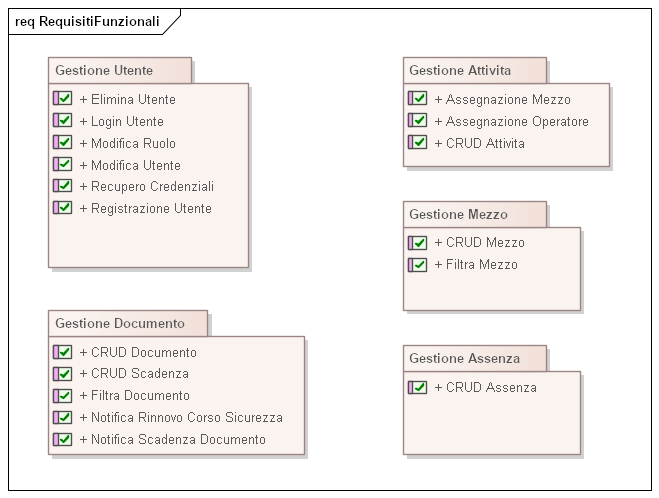
\includegraphics[width=1\textwidth]{RequisitiFunzionali}
\end{figure*}


\vphantom{space}\\[6cm]
\newsection{Requisiti Non Funzionali}

% Requisiti non funzionali (testo inserito automaticamente)
\newsubsection*{Area: Gestione Tecnologie}

\newsubsubsection*{RNF1: Implementazione in Python 3}

Il sistema dovrà essere implementato utilizzando Python 3.

\newsubsubsection*{RNF2: Utilizzo Database Relazionale}

Il sistema dovrà utilizzare un database relazionale per la gestione persistente dei dati.

\newsubsubsection*{RNF3: Verifica Email}

Il sistema dovrà prevedere la verifica dell'indirizzo email degli utenti durante la registrazione.

\newsubsubsection*{RNF4: Recupero Credenziali Tramite Email}

Il sistema dovrà permettere il recupero delle credenziali tramite email.

\newsubsection*{Area: Gestione UI/UX}

\newsubsubsection*{RNF5: Visualizzazione Turni con Calendario}

Il sistema dovrà offrire una visualizzazione dei turni tramite un calendario integrato.

\newsubsubsection*{RNF6: Interfaccia Responsive}

Il sistema dovrà presentare un'interfaccia responsive, fruibile da dispositivi con diverse risoluzioni.

\newsubsubsection*{RNF7: Notifica Scadenza Compilazione Documento}

Il sistema dovrà inviare notifiche relative alla scadenza della compilazione dei documenti entro 24 ore quando mancano 10 giorni alla scadenza.

\newsubsubsection*{RNF8: Notifica Eliminazione Documento}

Il sistema dovrà inviare notifiche 30 giorni prima dell'eliminazione di un documento al termine del periodo minimo di archiviazione di 3 anni.

\begin{figure*}[ht]
    \centering
    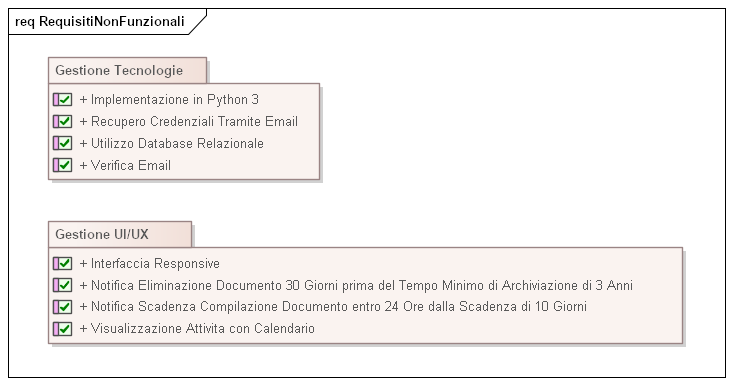
\includegraphics[width=1\textwidth]{RequisitiNonFunzionali}
\end{figure*}


\clearpage
\newsection{Tabella MoSCoW dei Requisiti}

Di seguito la matrice MoSCoW che classifica i requisiti del sistema secondo le priorità: M (Must-have), S (Should-have), C (Could-have), W (Won't-have).

\begin{longtable}{|p{4.5cm}|p{6.25cm}|p{2cm}|}
\hline
	\textbf{Area} & \textbf{Requisito} & \textbf{Priorità MoSCoW} \\
\hline
\endhead

Gestione Utente & RF1: Registrazione Utente & Must \\
\hline
Gestione Utente & RF2: Login Utente & Must \\
\hline
Gestione Utente & RF3: Recupero Credenziali & Should \\
\hline
Gestione Utente & RF4: Visualizza Utente & Must \\
\hline
Gestione Utente & RF5: Modifica Ruolo & Should \\
\hline
Gestione Utente & RF6: Modifica Utente & Should \\
\hline
Gestione Utente & RF7: Elimina Utente & Must \\
\hline
Gestione Assenza & RF8: CRUD Assenza & Should \\
\hline
Gestione Attività & RF9: CRUD Attività - carico/scarico & Must \\
\hline
Gestione Attività & RF10: Assegnazione Operatore & Must \\
\hline
Gestione Attività & RF11: Assegnazione Mezzo & Must \\
\hline
Gestione Documento & RF12: CRUD Documento FIR & Must \\
\hline
Gestione Documento & RF13: Filtra Documento & Should \\
\hline
Gestione Documento & RF14: Notifica Rinnovo Corso Sicurezza & Could \\
\hline
Gestione Documento & RF15: Notifica Scadenza Documento & Should \\
\hline
Gestione Mezzo & RF16: CRUD Mezzo & Must \\
\hline
Gestione Mezzo & RF17: Filtra Mezzo & Should \\
\hline
Gestione Tecnologie & RNF1: Implementazione in Python 3 & Must \\
\hline
Gestione Tecnologie & RNF2: Utilizzo Database Relazionale & Must \\
\hline
Gestione Tecnologie & RNF3: Verifica Email & Should \\
\hline
Gestione Tecnologie & RNF4: Recupero Credenziali tramite Email & Should \\
\hline
Gestione UI/UX & RNF5: Visualizzazione Turni con Calendario & Could \\
\hline
Gestione UI/UX & RNF6: Interfaccia Responsive & Should \\
\hline
Gestione UI/UX & RNF7: Notifica Scadenza Compilazione Documento & Should \\
\hline
Gestione UI/UX & RNF8: Notifica Eliminazione Documento & Won't \\
\hline
\end{longtable}

\clearpage
\newsection{Diagrammi dei Casi d'Uso}

\newsubsection*{Diagramma degli Attori}
Il diagramma individua gli attori coinvolti nel sistema e visualizza le connessioni di ereditarietà tra di essi.

\begin{figure*}[ht]
    \centering
    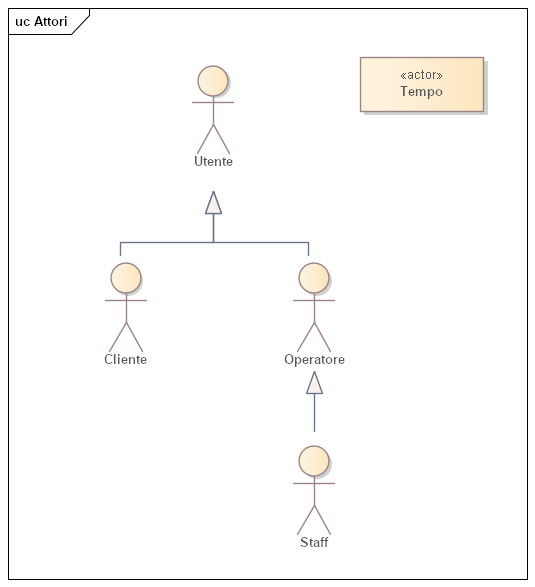
\includegraphics[width=1\textwidth]{Attori}
\end{figure*}

\clearpage
\newsubsection*{Gestione Utente}

Il diagramma evidenzia le relazioni tra attori e casi d’uso per la gestione degli utenti, incluse registrazione, autenticazione, assegnazione di ruoli e modifica dei profili.

\begin{figure*}[ht]
    \centering
    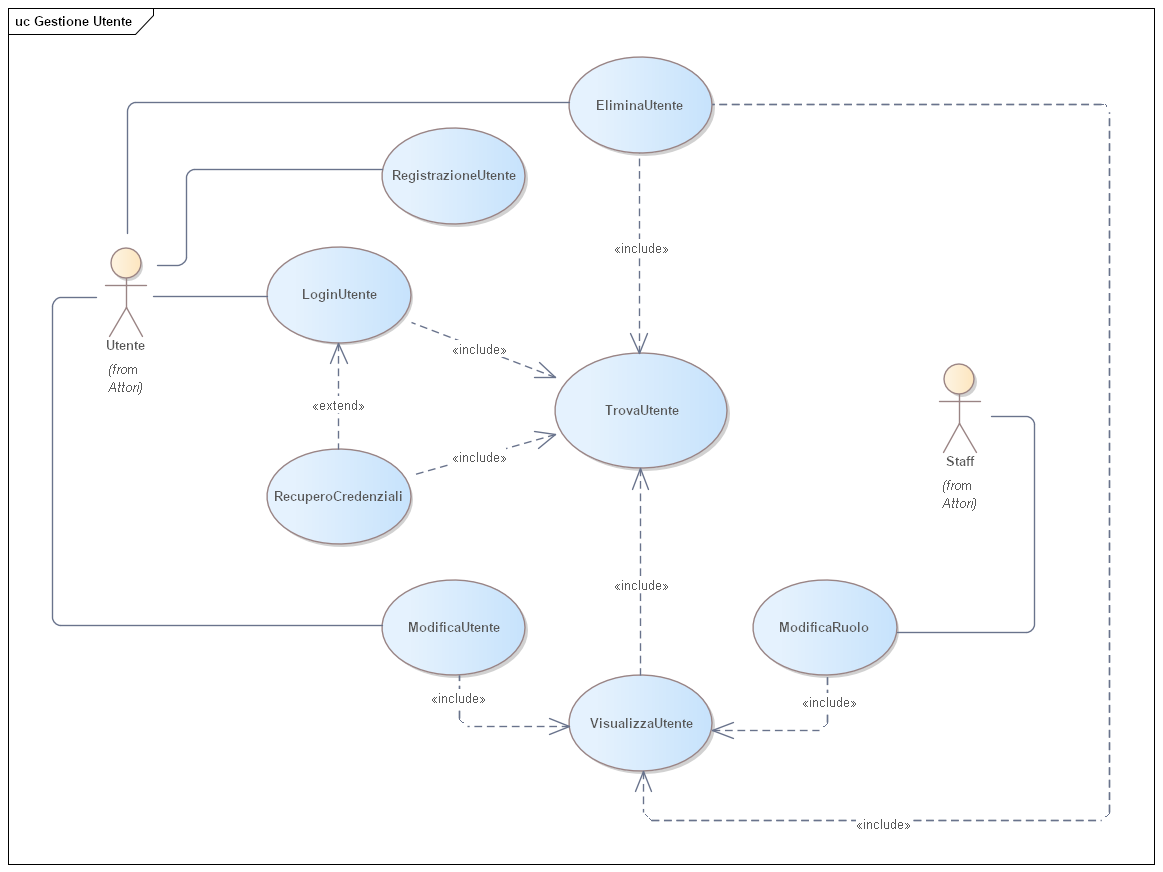
\includegraphics[width=1\textwidth]{GestioneUtente}
\end{figure*}

\clearpage
\begin{table}[H]
\vspace*{-0cm}
\renewcommand{\arraystretch}{1.9}
\begin{tabular}{|p{3.9cm}|p{9.9cm}|}
\hline
\multicolumn{2}{|c|}{\textbf{Caso d’uso: RegistrazioneUtente}} \\ \hline
\textbf{ID} & 1 \\ \hline
\textbf{Breve descrizione} & L'Utente si registra nel sistema, con un ruolo che dipende dal punto di accesso \\ \hline
\textbf{Attori primari} & Utente, Staff \\ \hline
\textbf{Attori secondari} & Nessuno \\ \hline
\textbf{Precondizioni} & Nessuna \\ \hline
\textbf{Sequenza degli eventi principale} &
\begin{enumerate}[leftmargin=14pt,label=\arabic*.,labelsep=0.5em,topsep=0pt,partopsep=0pt,parsep=0pt,itemsep=0pt]
    \item \texttt{If} l'Utente è un Cliente che accede alla pagina di registrazione pubblica, allora
    \begin{enumerate}[label=\arabic{enumi}.\arabic*.,leftmargin=22pt,labelsep=0.5em,topsep=0pt,partopsep=0pt,parsep=0pt,itemsep=0pt]
        \item Il sistema mostra il modulo di registrazione
        \item Il Cliente inserisce le proprie informazioni (nome, cognome, email, password)
        \item Il sistema valida i dati inseriti
        \item Il sistema crea un nuovo account con il ruolo di Cliente
    \end{enumerate}
\end{enumerate}\\ \hline
\textbf{Postcondizioni} & 
\begin{enumerate}[leftmargin=14pt,label=\arabic*.,labelsep=0.5em,topsep=0pt,partopsep=0pt,parsep=0pt,itemsep=0pt]
\item È stato creato un nuovo account utente con un ruolo specifico (Cliente, Operatore o Staff) 
\end{enumerate} \\ \hline
\textbf{Sequenza degli eventi alternativa} & \begin{enumerate}[leftmargin=14pt,label=\arabic*.,labelsep=0.5em,topsep=0pt,partopsep=0pt,parsep=0pt,itemsep=0pt]
    \item \texttt{If} l'Utente è un membro dello Staff che accede alla pagina di gestione utenti interna, allora
    \begin{enumerate}[label=\arabic{enumi}.\arabic*.,leftmargin=22pt,labelsep=0.5em,topsep=0pt,partopsep=0pt,parsep=0pt,itemsep=0pt]
        \item Il sistema mostra un modulo di creazione utente
        \item Il membro dello Staff inserisce le informazioni del nuovo utente (nome, cognome, email, password) e seleziona il ruolo desiderato (Operatore o Staff)
        \item Il sistema valida i dati inseriti
        \item Il sistema crea un nuovo account con il ruolo specificato (Operatore o Staff)
    \end{enumerate}
\end{enumerate}\\ \hline
\end{tabular}
\end{table}

\clearpage
\begin{table}[H]
\vspace*{-0cm}
\renewcommand{\arraystretch}{1.9}
\begin{tabular}{|p{3.9cm}|p{9.9cm}|}
\hline
\multicolumn{2}{|c|}{\textbf{Caso d’uso: LoginUtente}} \\ \hline
\textbf{ID} & 2 \\ \hline
\textbf{Breve descrizione} &  Permette all’Utente di accedere al proprio account\\ \hline
\textbf{Attori primari} & Utente \\ \hline
\textbf{Attori secondari} & Nessuno \\ \hline
\textbf{Precondizioni} & \begin{enumerate}[leftmargin=14pt,label=\arabic*.,labelsep=0.5em,topsep=0pt,partopsep=0pt,parsep=0pt,itemsep=0pt]
    \item L’Utente deve essere già registrato nel sistema 
\end{enumerate}\\ \hline
\textbf{Sequenza degli eventi principale} & \begin{enumerate}[leftmargin=14pt,label=\arabic*.,labelsep=0.5em,topsep=0pt,partopsep=0pt,parsep=0pt,itemsep=0pt]
    \item Il caso d’uso inizia quando l’Utente inserirsce le credenziali e seleziona "Accedi" \newline \texttt{Extend} \textit{RecuperaCredenziali}
    \item \texttt{While} le credenziali inserite dall’Utente non sono valide
    \begin{enumerate}[label=\arabic{enumi}.\arabic*.,leftmargin=22pt,labelsep=0.5em,topsep=0pt,partopsep=0pt,parsep=0pt,itemsep=0pt]
        \item Il sistema richiede all’Utente di inserire email e password
        \item Il sistema valida le credenziali fornite
    \end{enumerate}
    \item Il sistema autentica l’Utente e lo reindirizza alla pagina principale/area riservata
\end{enumerate}\\ \hline
\textbf{Postcondizioni} & \begin{enumerate}[leftmargin=14pt,label=\arabic*.,labelsep=0.5em,topsep=0pt,partopsep=0pt,parsep=0pt,itemsep=0pt]
    \item L’Utente ha effettuato il login al proprio account e può accedere alle funzionalità autorizzate
    \end{enumerate} \\ \hline
\textbf{Sequenza degli eventi alternativa} & Nessuna \\ \hline
\end{tabular}
\end{table}

\clearpage
\begin{table}[H]
\vspace*{-0cm}
\renewcommand{\arraystretch}{1.9}
\begin{tabular}{|p{3.9cm}|p{9.9cm}|}
\hline
\multicolumn{2}{|c|}{\textbf{Caso d’uso: RecuperaCredenziali}} \\ \hline
\textbf{ID} & 3 \\ \hline
\textbf{Breve descrizione} & L’Utente recupera le credenziali del proprio account in caso di smarrimento o dimenticanza della password \\ \hline
\textbf{Attori primari} & Utente \\ \hline
\textbf{Attori secondari} & Nessuno \\ \hline
\textbf{Precondizioni} & \begin{enumerate}[leftmargin=14pt,label=\arabic*.,labelsep=0.5em,topsep=0pt,partopsep=0pt,parsep=0pt,itemsep=0pt]
    \item L'Utente ha un account registrato nel sistema
    \item L'Utente visualizza la schermata di login
\end{enumerate} \\ \hline
\textbf{Sequenza degli eventi principale} &
\begin{enumerate}[leftmargin=14pt,label=\arabic*.,labelsep=0.5em,topsep=0pt,partopsep=0pt,parsep=0pt,itemsep=0pt]
    \item Il caso d'uso inizia quando l'Utente seleziona l’opzione "Recupera credenziali"
    \item \texttt{While} l'Utente non ha inserito l'email
    \begin{enumerate}[label=\arabic{enumi}.\arabic*.,leftmargin=22pt,labelsep=0.5em,topsep=0pt,partopsep=0pt,parsep=0pt,itemsep=0pt]
        \item Il sistema richiede all’Utente di inserire la propria email
        \item Il sistema valida la correttezza e l’esistenza dell’email nel sistema
    \end{enumerate}
    \item Il sistema genera una procedura di recupero (es. invio di un link sicuro o generazione temporanea di una nuova password) e invia le istruzioni all’indirizzo email fornito
    \item L'Utente riceve la mail, segue la procedura indicata e utilizza la nuova password o il link per ripristinare l’accesso al proprio account
\end{enumerate}\\ \hline
\textbf{Postcondizioni} & \begin{enumerate}[leftmargin=14pt,label=\arabic*.,labelsep=0.5em,topsep=0pt,partopsep=0pt,parsep=0pt,itemsep=0pt]
    \item L’Utente ha ricevuto le istruzioni per recuperare l’accesso al proprio account
    \item L’Utente può accedere nuovamente al sistema utilizzando la nuova password o il link fornito
    \end{enumerate} \\ \hline
\textbf{Sequenza degli eventi alternativa} & Nessuna \\ \hline
\end{tabular}
\end{table}

\clearpage
\begin{table}[H]
\vspace*{-0cm}
\renewcommand{\arraystretch}{1.9}
\begin{tabular}{|p{3.9cm}|p{9.9cm}|}
\hline
\multicolumn{2}{|c|}{\textbf{Caso d’uso: VisualizzaUtente}} \\ \hline
\textbf{ID} & 4 \\ \hline
\textbf{Breve descrizione} & L’Utente visualizza i propri dati anagrafici e le informazioni \\ \hline
\textbf{Attori primari} & Utente \\ \hline
\textbf{Attori secondari} & Nessuno \\ \hline
\textbf{Precondizioni} & \begin{enumerate}[leftmargin=14pt,label=\arabic*.,labelsep=0.5em,topsep=0pt,partopsep=0pt,parsep=0pt,itemsep=0pt]
    \item L’Utente è stato autenticato dal sistema
\end{enumerate} \\ \hline
\textbf{Sequenza degli eventi principale} &
\begin{enumerate}[leftmargin=14pt,label=\arabic*.,labelsep=0.5em,topsep=0pt,partopsep=0pt,parsep=0pt,itemsep=0pt]
    \item Il caso d'uso inizia quando l'Utente seleziona l'opzione di visualizzazione del proprio profilo
    \item Il sistema mostra i dati anagrafici  e le informazioni relative all’Utente
\end{enumerate}\\ \hline
\textbf{Postcondizioni} & \begin{enumerate}[leftmargin=14pt,label=\arabic*.,labelsep=0.5em,topsep=0pt,partopsep=0pt,parsep=0pt,itemsep=0pt]
    \item All’Utente sono mostrati i propri dati
    \end{enumerate} \\ \hline
\textbf{Sequenza degli eventi alternativa} & \begin{enumerate}[leftmargin=14pt,label=\arabic*.,labelsep=0.5em,topsep=0pt,partopsep=0pt,parsep=0pt,itemsep=0pt] 
    \item \texttt{If} Lo Staff richiede la visualizzazione
    \begin{enumerate}[label=\arabic{enumi}.\arabic*.,leftmargin=22pt,labelsep=0.5em,topsep=0pt,partopsep=0pt,parsep=0pt,itemsep=0pt]
        \item \texttt{Extend} \textit{TrovaUtente} 
        \item Il sistema mostra l’elenco degli Operatori registrati
        \item Lo Staff seleziona un Operatore dall’elenco
        \item Il sistema mostra i dati anagrafici completi e le informazioni aggiuntive (ruolo, turni, assenze, attività corrente collegata)
    \end{enumerate}
\end{enumerate}\\ \hline
\end{tabular}
\end{table}

\clearpage
\begin{table}[H]
\vspace*{-0cm}
\renewcommand{\arraystretch}{1.9}
\begin{tabular}{|p{3.9cm}|p{9.9cm}|}
\hline
\multicolumn{2}{|c|}{\textbf{Caso d’uso: TrovaUtente}} \\ \hline
\textbf{ID} & 5 \\ \hline
\textbf{Breve descrizione} & Lo Staff esegue la ricerca di uno o più Utenti \\ \hline
\textbf{Attori primari} & Staff \\ \hline
\textbf{Attori secondari} & Nessuno \\ \hline
\textbf{Precondizioni} & \begin{enumerate}[leftmargin=14pt,label=\arabic*.,labelsep=0.5em,topsep=0pt,partopsep=0pt,parsep=0pt,itemsep=0pt]
    \item Lo Staff è stato autenticato dal sistema
\end{enumerate} \\ \hline
\textbf{Sequenza degli eventi principale} &
\begin{enumerate}[leftmargin=14pt,label=\arabic*.,labelsep=0.5em,topsep=0pt,partopsep=0pt,parsep=0pt,itemsep=0pt]
    \item Il caso d’uso inizia quando lo Staff inserisce il criterio di ricerca nella barra dedicata (es. nome, cognome, email, ecc.)
    \item Il sistema ricerca l’Utente che soddisfa i criteri desiderati dallo Staff
    \item \texttt{If} Il sistema trova uno o più utenti
    \begin{enumerate}[label=\arabic{enumi}.\arabic{enumii}.,leftmargin=22pt,labelsep=0.5em,topsep=0pt,partopsep=0pt,parsep=0pt,itemsep=0pt]
    \item \texttt{For Each} Utente trovato
    \begin{enumerate}[label=\arabic{enumi}.\arabic{enumii}.\arabic{enumiii}.,leftmargin=22pt,labelsep=0.5em,topsep=0pt,partopsep=0pt,parsep=0pt,itemsep=0pt]
        \item Il sistema mostra le informazioni base dell’Utente
    \end{enumerate}
    \end{enumerate}
    \item \texttt{Else} Il sistema comunica allo staff che non sono stati trovati Utenti che soddisfano i criteri specificati
\end{enumerate}\\ \hline
\textbf{Postcondizioni} & Nessuna \\ \hline
\textbf{Sequenza degli eventi alternativa} & Nessuna \\ \hline
\end{tabular}
\end{table}

\clearpage
\begin{table}[H]
\vspace*{-0cm}
\renewcommand{\arraystretch}{1.9}
\begin{tabular}{|p{3.9cm}|p{9.9cm}|}
\hline
\multicolumn{2}{|c|}{\textbf{Caso d’uso: ModificaRuolo}} \\ \hline
\textbf{ID} & 6 \\ \hline
\textbf{Breve descrizione} & Lo Staff modifica il ruolo all’Operatore e/o allo Staff \\ \hline
\textbf{Attori primari} & Staff \\ \hline
\textbf{Attori secondari} & Nessuno \\ \hline
\textbf{Precondizioni} & \begin{enumerate}[leftmargin=14pt,label=\arabic*.,labelsep=0.5em,topsep=0pt,partopsep=0pt,parsep=0pt,itemsep=0pt]
    \item Lo Staff è autenticato
    \item Lo Staff visualizza la sezione interna per la gestione degli utenti
\end{enumerate} \\ \hline
\textbf{Sequenza degli eventi principale} &
\begin{enumerate}[leftmargin=14pt,label=\arabic*.,labelsep=0.5em,topsep=0pt,partopsep=0pt,parsep=0pt,itemsep=0pt]
    \item Il caso d’uso inizia quando lo Staff seleziona l’Operatore da modificare
    \item Lo Staff può modificare il ruolo dell’Operatore
    \item \texttt{If} la modifica è confermata e i dati sono validi
    \begin{enumerate}[label=\arabic{enumi}.\arabic*.,leftmargin=22pt,labelsep=0.5em,topsep=0pt,partopsep=0pt,parsep=0pt,itemsep=0pt]
        \item Il sistema aggiorna il ruolo dell’Operatore
        \item \texttt{Include} \textit{VisualizzaUtente}
    \end{enumerate}
\end{enumerate}\\ \hline
\textbf{Postcondizioni} & \begin{enumerate}[leftmargin=14pt,label=\arabic*.,labelsep=0.5em,topsep=0pt,partopsep=0pt,parsep=0pt,itemsep=0pt]
    \item Il ruolo dell’Operatore è stato modificato
    \end{enumerate} \\ \hline
\textbf{Sequenza degli eventi alternativa} & Nessuna\\ \hline
\end{tabular}
\end{table}

\clearpage
\begin{table}[H]
\vspace*{-0cm}
\renewcommand{\arraystretch}{1.9}
\begin{tabular}{|p{3.9cm}|p{9.9cm}|}
\hline
\multicolumn{2}{|c|}{\textbf{Caso d’uso: ModificaUtente}} \\ \hline
\textbf{ID} & 7 \\ \hline
\textbf{Breve descrizione} &  L’Utente modifica i propri dati anagrafici \\ \hline
\textbf{Attori primari} & Utente \\ \hline
\textbf{Attori secondari} & Nessuno \\ \hline
\textbf{Precondizioni} & \begin{enumerate}[leftmargin=14pt,label=\arabic*.,labelsep=0.5em,topsep=0pt,partopsep=0pt,parsep=0pt,itemsep=0pt]
    \item L’Utente è stato autenticato dal sistema
\end{enumerate} \\ \hline
\textbf{Sequenza degli eventi principale} &
\begin{enumerate}[leftmargin=14pt,label=\arabic*.,labelsep=0.5em,topsep=0pt,partopsep=0pt,parsep=0pt,itemsep=0pt]
    \item Il caso d'uso inizia quando l’Utente seleziona l'opzione di modifica del profilo
    \item L'Utente modifica i dati desiderati
    \item \texttt{If} I dati inseriti sono validi
    \begin{enumerate}[label=\arabic{enumi}.\arabic*.,leftmargin=22pt,labelsep=0.5em,topsep=0pt,partopsep=0pt,parsep=0pt,itemsep=0pt]
        \item Il sistema aggiorna i dati modificati
        \item \texttt{Include} \textit{(VisualizzaUtente)} 
    \end{enumerate}
    \item \texttt{Else}
    \begin{enumerate}[label=\arabic{enumi}.\arabic*.,leftmargin=22pt,labelsep=0.5em,topsep=0pt,partopsep=0pt,parsep=0pt,itemsep=0pt]
        \item Il sistema mostra un messaggio di errore e richiede una nuova modifica
    \end{enumerate}
\end{enumerate}\\ \hline
\textbf{Postcondizioni} & \begin{enumerate}[leftmargin=14pt,label=\arabic*.,labelsep=0.5em,topsep=0pt,partopsep=0pt,parsep=0pt,itemsep=0pt]
    \item I dati anagrafici dell’Utente vengono aggiornati nel sistema
    \end{enumerate} \\ \hline
\textbf{Sequenza degli eventi alternativa} & \begin{enumerate}[leftmargin=14pt,label=\arabic*.,labelsep=0.5em,topsep=0pt,partopsep=0pt,parsep=0pt,itemsep=0pt] 
    \item Lo Staff richiede la modifica
    \item Il sistema mostra l’elenco di tutti gli Operatori registrati
    \item Lo Staff seleziona l’Operatore da modificare dall’elenco
    \item Lo Staff modifica i dati desiderati
    \item \texttt{If} I dati inseriti sono validi
    \begin{enumerate}[label=\arabic{enumi}.\arabic*.,leftmargin=22pt,labelsep=0.5em,topsep=0pt,partopsep=0pt,parsep=0pt,itemsep=0pt]
        \item Il sistema aggiorna i dati modificati
    \end{enumerate}
    \item \texttt{Else}
    \begin{enumerate}[label=\arabic{enumi}.\arabic*.,leftmargin=22pt,labelsep=0.5em,topsep=0pt,partopsep=0pt,parsep=0pt,itemsep=0pt]
        \item Il sistema mostra un messaggio di errore e richiede una nuova modifica
    \end{enumerate}
\end{enumerate}\\ \hline
\end{tabular}
\end{table}

\clearpage
\begin{table}[H]
\vspace*{-0cm}
\renewcommand{\arraystretch}{1.9}
\begin{tabular}{|p{3.9cm}|p{9.9cm}|}
\hline
\multicolumn{2}{|c|}{\textbf{Caso d’uso: EliminaUtente}} \\ \hline
\textbf{ID} & 8 \\ \hline
\textbf{Breve descrizione} &  L’Utente elimina il proprio account \\ \hline
\textbf{Attori primari} & Utente \\ \hline
\textbf{Attori secondari} & Nessuno \\ \hline
\textbf{Precondizioni} & \begin{enumerate}[leftmargin=14pt,label=\arabic*.,labelsep=0.5em,topsep=0pt,partopsep=0pt,parsep=0pt,itemsep=0pt]
    \item L’Utente è stato autenticato dal sistema
\end{enumerate} \\ \hline
\textbf{Sequenza degli eventi principale} &
\begin{enumerate}[leftmargin=14pt,label=\arabic*.,labelsep=0.5em,topsep=0pt,partopsep=0pt,parsep=0pt,itemsep=0pt]
    \item Il caso d'uso inizia quando l’Utente seleziona l'opzione di eliminazione del profilo
    \item \texttt{If} L’Utente conferma l’operazione
    \begin{enumerate}[label=\arabic{enumi}.\arabic*.,leftmargin=22pt,labelsep=0.5em,topsep=0pt,partopsep=0pt,parsep=0pt,itemsep=0pt]
        \item Il sistema elimina l’Utente e mostra un messaggio di conferma
    \end{enumerate}
    \item \texttt{Else}
    \begin{enumerate}[label=\arabic{enumi}.\arabic*.,leftmargin=22pt,labelsep=0.5em,topsep=0pt,partopsep=0pt,parsep=0pt,itemsep=0pt]
        \item Il sistema annulla l’operazione e non apporta modifiche
    \end{enumerate}
\end{enumerate}\\ \hline
\textbf{Postcondizioni} & \begin{enumerate}[leftmargin=14pt,label=\arabic*.,labelsep=0.5em,topsep=0pt,partopsep=0pt,parsep=0pt,itemsep=0pt]
    \item \texttt{If} confermato
    \begin{enumerate}[label=\arabic{enumi}.\arabic*.,leftmargin=22pt,labelsep=0.5em,topsep=0pt,partopsep=0pt,parsep=0pt,itemsep=0pt]
        \item L’Utente selezionato viene rimosso dal sistema
    \end{enumerate}
\end{enumerate} \\ \hline
\textbf{Sequenza degli eventi alternativa} & \begin{enumerate}[leftmargin=14pt,label=\arabic*.,labelsep=0.5em,topsep=0pt,partopsep=0pt,parsep=0pt,itemsep=0pt] 
    \item Il caso d'uso inizia quando lo Staff seleziona l'opzione di eliminazione del profilo dall'elenco
    \item \texttt{If} Lo Staff conferma l’operazione
    \begin{enumerate}[label=\arabic{enumi}.\arabic*.,leftmargin=22pt,labelsep=0.5em,topsep=0pt,partopsep=0pt,parsep=0pt,itemsep=0pt]
        \item Il sistema elimina l’Utente e mostra un messaggio di conferma
    \end{enumerate}
    \item \texttt{Else}
    \begin{enumerate}[label=\arabic{enumi}.\arabic*.,leftmargin=22pt,labelsep=0.5em,topsep=0pt,partopsep=0pt,parsep=0pt,itemsep=0pt]
        \item Il sistema annulla l’operazione e non apporta modifiche
\end{enumerate}
\end{enumerate}\\ \hline
\end{tabular}
\end{table}



\clearpage
\newsubsection*{Gestione Assenza}

La sottosezione descrive i casi d'uso relativi alla gestione delle assenze del personale (ferie, malattia, permessi). In questa area sono documentate le operazioni principali: creazione, visualizzazione, modifica ed eliminazione delle assenze, con l'indicazione degli attori coinvolti (principalmente lo Staff) e delle precondizioni necessarie.

\begin{figure*}[ht]
    \centering
    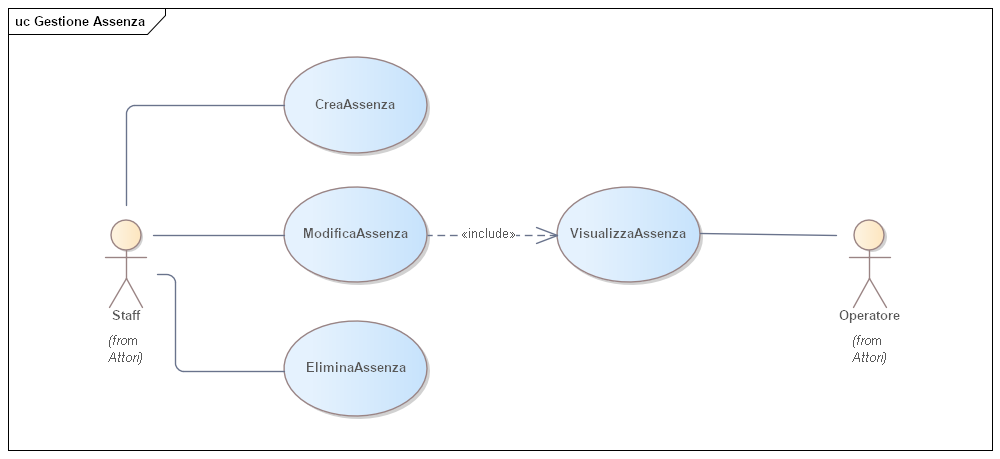
\includegraphics[width=1\textwidth]{GestioneAssenza}
\end{figure*}

\clearpage
\renewcommand{\arraystretch}{1.9}
\begin{table}[H]
\vspace*{-0cm}
\begin{tabular}{|p{3.9cm}|p{9.9cm}|}
\hline
\multicolumn{2}{|c|}{\textbf{Caso d’uso: CreaAssenza}} \\ \hline
\textbf{ID} & 9 \\ \hline
\textbf{Breve descrizione} & Lo Staff crea una nuova assenza (ferie, malattia, permesso) per un Operatore \\ \hline
\textbf{Attori primari} & Staff \\ \hline
\textbf{Attori secondari} & Nessuno \\ \hline
\textbf{Precondizioni} & \begin{enumerate}[leftmargin=14pt,label=\arabic*.,labelsep=0.5em,topsep=0pt,partopsep=0pt,parsep=0pt,itemsep=0pt]
    \item Lo Staff è autenticato.
    \item L’Operatore per cui viene registrata l’assenza esiste
\end{enumerate} \\ \hline
\textbf{Sequenza degli eventi principale} & \begin{enumerate}[leftmargin=14pt,label=\arabic*.,labelsep=0.5em,topsep=0pt,partopsep=0pt,parsep=0pt,itemsep=0pt]
    \item Il caso d’uso inizia quando lo Staff seleziona “Nuova assenza”
    \item Il sistema richiede i dati dell’assenza (tipo, data inizio, data fine)
    \item Lo Staff inserisce i dati
    \item \texttt{If} I dati sono validi
    \begin{enumerate}[label=\arabic{enumi}.\arabic*.,leftmargin=22pt,labelsep=0.5em,topsep=0pt,partopsep=0pt,parsep=0pt,itemsep=0pt]
        \item Il sistema registra l’assenza
        \item Il sistema mostra un messaggio di conferma
    \end{enumerate}
    \item \texttt{Else}
    \begin{enumerate}[label=\arabic{enumi}.\arabic*.,leftmargin=22pt,labelsep=0.5em,topsep=0pt,partopsep=0pt,parsep=0pt,itemsep=0pt]
        \item Il sistema mostra un errore e richiede la correzione
    \end{enumerate}
\end{enumerate} \\ \hline
\textbf{Postcondizioni} & \begin{enumerate}[label=\arabic*.,leftmargin=14pt,labelsep=0.5em,topsep=0pt,partopsep=0pt,parsep=0pt,itemsep=0pt]
        \item L’assenza è registrata nel sistema.
\end{enumerate} \\ \hline
\textbf{Sequenza degli eventi alternativa} & \begin{enumerate}[leftmargin=14pt,label=\arabic*.,labelsep=0.5em,topsep=0pt,partopsep=0pt,parsep=0pt,itemsep=0pt]
    \item \texttt{If} Lo Staff non conferma l’operazione
    \begin{enumerate}[label=\arabic{enumi}.\arabic*.,leftmargin=22pt,labelsep=0.5em,topsep=0pt,partopsep=0pt,parsep=0pt,itemsep=0pt]
        \item Il sistema annulla l’operazione e non apporta modifiche.
    \end{enumerate}
\end{enumerate} \\ \hline
\end{tabular}
\end{table}

\clearpage
\begin{table}[H]
\vspace*{-0cm}
\renewcommand{\arraystretch}{1.9}
\begin{tabular}{|p{3.9cm}|p{9.9cm}|}
\hline
\multicolumn{2}{|c|}{\textbf{Caso d’uso: VisualizzaAssenza}} \\ \hline
\textbf{ID} & 10 \\ \hline
\textbf{Breve descrizione} & L’Operatore visualizza le assenze registrate \\ \hline
\textbf{Attori primari} & Operatore \\ \hline
\textbf{Attori secondari} & Nessuno \\ \hline
\textbf{Precondizioni} & \begin{enumerate}[leftmargin=14pt,label=\arabic*.,labelsep=0.5em,topsep=0pt,partopsep=0pt,parsep=0pt,itemsep=0pt]
    \item L’Operatore è autenticato.
    \item Esistono assenze registrate.
\end{enumerate} \\ \hline
\textbf{Sequenza degli eventi principale} & \begin{enumerate}[leftmargin=14pt,label=\arabic*.,labelsep=0.5em,topsep=0pt,partopsep=0pt,parsep=0pt,itemsep=0pt]
    \item Il caso d’uso inizia quando l’Operatore seleziona l'assenza da visualizzare
    \item Il sistema mostra i dettagli dell’assenza selezionata
\end{enumerate} \\ \hline
\textbf{Postcondizioni} & \begin{enumerate}[label=\arabic*.,leftmargin=14pt,labelsep=0.5em,topsep=0pt,partopsep=0pt,parsep=0pt,itemsep=0pt]
        \item L’Operatore visualizza le informazioni sulle assenze.
\end{enumerate} \\ \hline
\textbf{Sequenza degli eventi alternativa} & Nessuna. \\ \hline
\end{tabular}
\end{table}

\clearpage
\begin{table}[H]
\vspace*{-0cm}
\renewcommand{\arraystretch}{1.9}
\begin{tabular}{|p{3.9cm}|p{9.9cm}|}
\hline
\multicolumn{2}{|c|}{\textbf{Caso d’uso: ModificaAssenza}} \\ \hline
\textbf{ID} & 11 \\ \hline
\textbf{Breve descrizione} & Lo Staff modifica i dati di un’assenza esistente \\ \hline
\textbf{Attori primari} & Staff \\ \hline
\textbf{Attori secondari} & Nessuno \\ \hline
\textbf{Precondizioni} & \begin{enumerate}[leftmargin=14pt,label=\arabic*.,labelsep=0.5em,topsep=0pt,partopsep=0pt,parsep=0pt,itemsep=0pt]
    \item Lo Staff è autenticato.
    \item L’assenza esiste nel sistema.
\end{enumerate} \\ \hline
\textbf{Sequenza degli eventi principale} & \begin{enumerate}[leftmargin=14pt,label=\arabic*.,labelsep=0.5em,topsep=0pt,partopsep=0pt,parsep=0pt,itemsep=0pt]
    \item Il caso d’uso inizia quando lo Staff seleziona l’assenza da modificare.
    \item Lo Staff aggiorna i dati.
    \item \texttt{If} I dati modificati sono validi
    \begin{enumerate}[label=\arabic{enumi}.\arabic*.,leftmargin=22pt,labelsep=0.5em,topsep=0pt,partopsep=0pt,parsep=0pt,itemsep=0pt]
    \item Il sistema aggiorna l’assenza.
    \item \texttt{Include} \textit{(VisualizzaAssenza)}
    \end{enumerate}
    \item \texttt{Else}
    \begin{enumerate}[label=\arabic{enumi}.\arabic*.,leftmargin=22pt,labelsep=0.5em,topsep=0pt,partopsep=0pt,parsep=0pt,itemsep=0pt]
        \item Il sistema mostra un errore e non applica le modifiche.
    \end{enumerate}
\end{enumerate} \\ \hline
\textbf{Postcondizioni} & \begin{enumerate}[label=\arabic*.,leftmargin=14pt,labelsep=0.5em,topsep=0pt,partopsep=0pt,parsep=0pt,itemsep=0pt]
        \item L’assenza è aggiornata nel sistema.
\end{enumerate} \\ \hline
\textbf{Sequenza degli eventi alternativa} & \begin{enumerate}[leftmargin=14pt,label=\arabic*.,labelsep=0.5em,topsep=0pt,partopsep=0pt,parsep=0pt,itemsep=0pt]
    \item \texttt{If} Lo Staff non conferma l’operazione
    \begin{enumerate}[label=\arabic{enumi}.\arabic*.,leftmargin=22pt,labelsep=0.5em,topsep=0pt,partopsep=0pt,parsep=0pt,itemsep=0pt]
        \item Il sistema annulla l’operazione e non apporta modifiche.
    \end{enumerate}
\end{enumerate} \\ \hline
\end{tabular}
\end{table}

\clearpage
\begin{table}[H]
\vspace*{-0cm}
\renewcommand{\arraystretch}{1.9}
\begin{tabular}{|p{3.9cm}|p{9.9cm}|}
\hline
\multicolumn{2}{|c|}{\textbf{Caso d’uso: EliminaAssenza}} \\ \hline
\textbf{ID} & 12 \\ \hline
\textbf{Breve descrizione} & Lo Staff elimina un’assenza registrata. \\ \hline
\textbf{Attori primari} & Staff \\ \hline
\textbf{Attori secondari} & Nessuno \\ \hline
\textbf{Precondizioni} & \begin{enumerate}[leftmargin=14pt,label=\arabic*.,labelsep=0.5em,topsep=0pt,partopsep=0pt,parsep=0pt,itemsep=0pt]
    \item Lo Staff è autenticato.
    \item L’assenza esiste nel sistema.
\end{enumerate} \\ \hline
\textbf{Sequenza degli eventi principale} & \begin{enumerate}[leftmargin=14pt,label=\arabic*.,labelsep=0.5em,topsep=0pt,partopsep=0pt,parsep=0pt,itemsep=0pt]
    \item Il caso d'uso inizia quando lo Staff seleziona l'opzione di eliminazione dell'assenza
    \item Il sistema elimina l'assenza e mostra un messaggio di conferma
\end{enumerate} \\ \hline
\textbf{Postcondizioni} & \begin{enumerate}[label=\arabic*.,leftmargin=14pt,labelsep=0.5em,topsep=0pt,partopsep=0pt,parsep=0pt,itemsep=0pt]
        \item L’assenza è eliminata.
\end{enumerate} \\ \hline
\textbf{Sequenza degli eventi alternativa} & \begin{enumerate}[leftmargin=14pt,label=\arabic*.,labelsep=0.5em,topsep=0pt,partopsep=0pt,parsep=0pt,itemsep=0pt]
    \item \texttt{If} Lo Staff non conferma l’operazione
    \begin{enumerate}[label=\arabic{enumi}.\arabic*.,leftmargin=22pt,labelsep=0.5em,topsep=0pt,partopsep=0pt,parsep=0pt,itemsep=0pt]
        \item Il sistema annulla l’operazione e non apporta modifiche.
    \end{enumerate}
\end{enumerate} \\ \hline
\end{tabular}
\end{table}

\clearpage
\newsubsection*{Gestione Mezzo}

Il diagramma evidenzia le relazioni tra attori e casi d’uso per la gestione dei mezzi, come anagrafica, manutenzione, disponibilità e scadenze assicurative.

\begin{figure*}[ht]
    \centering
    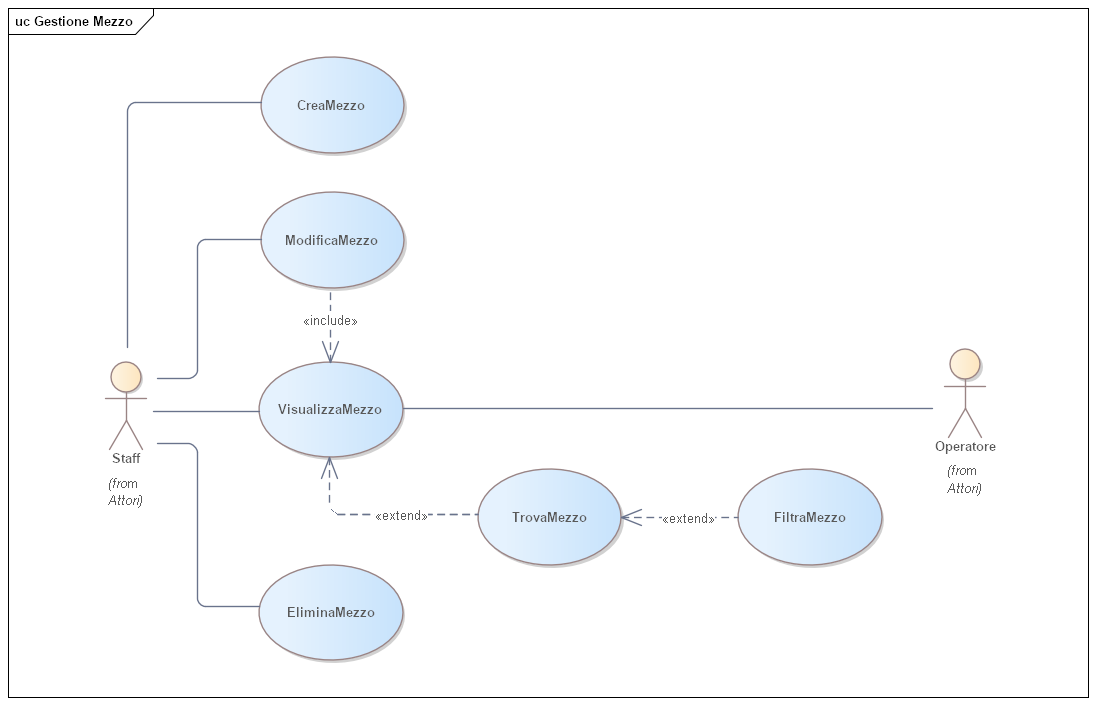
\includegraphics[width=1\textwidth]{GestioneMezzo}
\end{figure*}

\clearpage
\begin{table}[H]
\vspace*{-0cm}
\renewcommand{\arraystretch}{1.9}
\begin{tabular}{|p{3.9cm}|p{9.9cm}|}
\hline
\multicolumn{2}{|c|}{\textbf{Caso d’uso: CreaMezzo}} \\ \hline
	\textbf{ID} & 13 \\ \hline
	\textbf{Breve descrizione} & Lo Staff crea un nuovo mezzo nel sistema \\ \hline
	\textbf{Attori primari} & Staff \\ \hline
	\textbf{Attori secondari} & Nessuno \\ \hline
	\textbf{Precondizioni} & \begin{enumerate}[label=\arabic*.,leftmargin=14pt,labelsep=0.5em,topsep=0pt,partopsep=0pt,parsep=0pt,itemsep=0pt]
        \item Lo Staff è stato autenticato dal sistema
    \end{enumerate} \\ \hline
	\textbf{Sequenza degli eventi principale} &
\begin{enumerate}[leftmargin=14pt,label=\arabic*.,labelsep=0.5em,topsep=0pt,partopsep=0pt,parsep=0pt,itemsep=0pt]
    \item Il caso d’uso inizia quando lo Staff seleziona l'opzione di creazione di un nuovo mezzo
    \item Il sistema richiede l’inserimento dei dati (targa, modello, anno, categoria, stato)
    \item Lo Staff inserisce i dati
    \item \texttt{If} i dati inseriti sono validi e non duplicati
    \begin{enumerate}[label=\arabic{enumi}.\arabic*.,leftmargin=22pt,labelsep=0.5em,topsep=0pt,partopsep=0pt,parsep=0pt,itemsep=0pt]
        \item Il sistema registra il nuovo mezzo
        \item Il sistema mostra un messaggio di conferma
    \end{enumerate}
    \item \texttt{Else}
    \begin{enumerate}[label=\arabic{enumi}.\arabic*.,leftmargin=22pt,labelsep=0.5em,topsep=0pt,partopsep=0pt,parsep=0pt,itemsep=0pt]
        \item Il sistema mostra un messaggio di errore e richiede la correzione dei dati
    \end{enumerate}
\end{enumerate}\\ \hline
    	\textbf{Postcondizioni} & \begin{enumerate}[label=\arabic*.,leftmargin=14pt,labelsep=0.5em,topsep=0pt,partopsep=0pt,parsep=0pt,itemsep=0pt]
        \item Il nuovo mezzo è registrato nel sistema
        \end{enumerate} \\ \hline
    	\textbf{Sequenza degli eventi alternativa} &
\begin{enumerate}[leftmargin=14pt,label=\arabic*.,labelsep=0.5em,topsep=0pt,partopsep=0pt,parsep=0pt,itemsep=0pt]
    \item \texttt{If} lo Staff non conferma l’operazione
    \begin{enumerate}[label=\arabic{enumi}.\arabic*.,leftmargin=22pt,labelsep=0.5em,topsep=0pt,partopsep=0pt,parsep=0pt,itemsep=0pt]
        \item Il sistema annulla l’operazione e non apporta modifiche.
    \end{enumerate}
\end{enumerate} \\ \hline
\end{tabular}
\end{table}


\clearpage
\begin{table}[H]
\vspace*{-0cm}
\renewcommand{\arraystretch}{1.9}
\begin{tabular}{|p{3.9cm}|p{9.9cm}|}
\hline
\multicolumn{2}{|c|}{\textbf{Caso d’uso: VisualizzaMezzo}} \\ \hline
	\textbf{ID} & 14 \\ \hline
	\textbf{Breve descrizione} & L'Operatore visualizza i dati di un mezzo. \\ \hline
	\textbf{Attori primari} & Operatore \\ \hline
	\textbf{Attori secondari} & Nessuno \\ \hline
	\textbf{Precondizioni} & \begin{enumerate}[label=\arabic*.,leftmargin=14pt,labelsep=0.5em,topsep=0pt,partopsep=0pt,parsep=0pt,itemsep=0pt]
        \item L’Operatore è stato autenticato dal sistema
        \item Il mezzo da visualizzare esiste nel sistema.
    \end{enumerate} \\ \hline
    	\textbf{Sequenza degli eventi principale} & \begin{enumerate}[label=\arabic*.,leftmargin=14pt,labelsep=0.5em,topsep=0pt,partopsep=0pt,parsep=0pt,itemsep=0pt]
        \item Il caso d'uso inizia quando l'Operatore seleziona il mezzo da visualizzare
        \item Il sistema mostra i dati del mezzo (targa, modello, stato, ecc.)
    \end{enumerate}\\ \hline
    	\textbf{Postcondizioni} & \begin{enumerate}[label=\arabic*.,leftmargin=14pt,labelsep=0.5em,topsep=0pt,partopsep=0pt,parsep=0pt,itemsep=0pt]
        \item I dati del mezzo selezionato vengono visualizzati.
    \end{enumerate}\\ \hline
    	\textbf{Sequenza degli eventi alternativa} & \begin{enumerate}[leftmargin=14pt,label=\arabic*.,labelsep=0.5em,topsep=0pt,partopsep=0pt,parsep=0pt,itemsep=0pt]
        \item \texttt{If} Lo Staff richiede la visualizzazione
        \begin{enumerate}[label=\arabic{enumi}.\arabic*.,leftmargin=22pt,labelsep=0.5em,topsep=0pt,partopsep=0pt,parsep=0pt,itemsep=0pt]
            \item \texttt{Extend} \textit{TrovaMezzo}
            \item Lo Staff seleziona il mezzo da visualizzare
            \item Il sistema mostra i dati del mezzo (targa, modello, stato, ecc.)
        \end{enumerate}
    \end{enumerate} \\ \hline
\end{tabular}
\end{table}

\clearpage
\begin{table}[H]
\vspace*{-0cm}
\renewcommand{\arraystretch}{1.9}
\begin{tabular}{|p{3.9cm}|p{9.9cm}|}
\hline
\multicolumn{2}{|c|}{\textbf{Caso d’uso: TrovaMezzo}} \\ \hline
        extbf{ID} & 15 \\ \hline
        extbf{Breve descrizione} & Lo Staff esegue la ricerca di uno o più mezzi \\ \hline
	\textbf{Attori primari} & Staff \\ \hline
	\textbf{Attori secondari} & Nessuno \\ \hline
	\textbf{Precondizioni} & \begin{enumerate}[label=\arabic*.,leftmargin=14pt,labelsep=0.5em,topsep=0pt,partopsep=0pt,parsep=0pt,itemsep=0pt]
        \item Lo Staff è stato autenticato dal sistema
    \end{enumerate} \\ \hline
	\textbf{Sequenza degli eventi principale} & 
\begin{enumerate}[leftmargin=14pt,label=\arabic*.,labelsep=0.5em,topsep=0pt,partopsep=0pt,parsep=0pt,itemsep=0pt]
    \item Il caso d’uso inizia quando lo Staff inserisce il singolo criterio di ricerca nella barra dedicata (es. nome, targa)
    \item \texttt{Extend} \textit{FiltraMezzo}
    \item \texttt{While} il criterio di ricerca non è vuoto
    \begin{enumerate}[label=\arabic{enumi}.\arabic*.,leftmargin=22pt,labelsep=0.5em,topsep=0pt,partopsep=0pt,parsep=0pt,itemsep=0pt]
        \item Il sistema trova i mezzi corrispondenti.
        \item \texttt{If} viene trovato almeno un mezzo
        \begin{enumerate}[label=\arabic{enumi}.\arabic{enumii}.\arabic*.,leftmargin=22pt,labelsep=0.5em,topsep=0pt,partopsep=0pt,parsep=0pt,itemsep=0pt]
            \item Il sistema mostra l’elenco dei mezzi corrispondenti.
        \end{enumerate}
        \item \texttt{Else}
        \begin{enumerate}[label=\arabic{enumi}.\arabic{enumii}.\arabic*.,leftmargin=22pt,labelsep=0.5em,topsep=0pt,partopsep=0pt,parsep=0pt,itemsep=0pt]
            \item Il sistema mostra il messaggio “Nessun mezzo trovato”.
        \end{enumerate}
    \end{enumerate}
\end{enumerate}\\ \hline
    	\textbf{Postcondizioni} & \begin{enumerate}[label=\arabic*.,leftmargin=14pt,labelsep=0.5em,topsep=0pt,partopsep=0pt,parsep=0pt,itemsep=0pt]
        \item Lo Staff visualizza l’elenco dei mezzi corrispondenti ai criteri.
        \end{enumerate} \\ \hline
    	\textbf{Sequenza degli eventi alternativa} & Nessuna. \\ \hline
\end{tabular}
\end{table}


\clearpage
\begin{table}[H]
\vspace*{-0cm}
\renewcommand{\arraystretch}{1.9}
\begin{tabular}{|p{3.9cm}|p{9.9cm}|}
\hline
\multicolumn{2}{|c|}{\textbf{Caso d’uso: FiltraMezzo}} \\ \hline
	\textbf{ID} & 16 \\ \hline
	\textbf{Breve descrizione} & Lo Staff filtra i mezzi in base a criteri avanzati (modello, stato, ecc.) \\ \hline
	\textbf{Attori primari} & Staff \\ \hline
	\textbf{Attori secondari} & Nessuno \\ \hline
	\textbf{Precondizioni} & \begin{enumerate}[label=\arabic*.,leftmargin=14pt,labelsep=0.5em,topsep=0pt,partopsep=0pt,parsep=0pt,itemsep=0pt]
        \item Lo Staff è stato autenticato dal sistema.
    \end{enumerate} \\ \hline
	\textbf{Sequenza degli eventi principale} & 
\begin{enumerate}[leftmargin=14pt,label=\arabic*.,labelsep=0.5em,topsep=0pt,partopsep=0pt,parsep=0pt,itemsep=0pt]
    \item Il caso d'uso inizia quando lo Staff applica uno o più filtri durante l'azione di ricerca del mezzo (es. modello, stato, ecc.)
    \item \texttt{If} esistono mezzi che rispettano i filtri
    \begin{enumerate}[label=\arabic{enumi}.\arabic*.,leftmargin=22pt,labelsep=0.5em,topsep=0pt,partopsep=0pt,parsep=0pt,itemsep=0pt]
        \item Il sistema mostra l’elenco dei mezzi filtrati
    \end{enumerate}
    \item \texttt{Else}
    \begin{enumerate}[label=\arabic{enumi}.\arabic*.,leftmargin=22pt,labelsep=0.5em,topsep=0pt,partopsep=0pt,parsep=0pt,itemsep=0pt]
        \item Il sistema mostra “Nessun mezzo corrisponde ai criteri di filtro”
    \end{enumerate}
\end{enumerate}\\ \hline
    	\textbf{Postcondizioni} & \begin{enumerate}[label=\arabic*.,leftmargin=14pt,labelsep=0.5em,topsep=0pt,partopsep=0pt,parsep=0pt,itemsep=0pt]
        \item Lo Staff visualizza l’elenco dei mezzi filtrati
        \end{enumerate} \\ \hline
    	\textbf{Sequenza degli eventi alternativa} & Nessuna \\ \hline
\end{tabular}
\end{table}

\clearpage
\begin{table}[H]
\vspace*{-0cm}
\renewcommand{\arraystretch}{1.9}
\begin{tabular}{|p{3.9cm}|p{9.9cm}|}
\hline
\multicolumn{2}{|c|}{\textbf{Caso d’uso: ModificaMezzo}} \\ \hline
	\textbf{ID} & 17 \\ \hline
	\textbf{Breve descrizione} & Lo Staff modifica i dati di un mezzo esistente \\ \hline
	\textbf{Attori primari} & Staff \\ \hline
	\textbf{Attori secondari} & Nessuno \\ \hline
	\textbf{Precondizioni} & \begin{enumerate}[label=\arabic*.,leftmargin=14pt,labelsep=0.5em,topsep=0pt,partopsep=0pt,parsep=0pt,itemsep=0pt]
        \item Lo Staff è stato autenticato dal sistema
        \item Il mezzo da modificare esiste nel sistema
    \end{enumerate} \\ \hline
	\textbf{Sequenza degli eventi principale} & 
\begin{enumerate}[leftmargin=14pt,label=\arabic*.,labelsep=0.5em,topsep=0pt,partopsep=0pt,parsep=0pt,itemsep=0pt]
    \item Il caso d'uso inizia quando lo Staff seleziona il mezzo da modificare
    \item Lo Staff modifica i dati del mezzo
    \item \texttt{If} i dati inseriti sono validi
    \begin{enumerate}[label=\arabic{enumi}.\arabic*.,leftmargin=22pt,labelsep=0.5em,topsep=0pt,partopsep=0pt,parsep=0pt,itemsep=0pt]
        \item Il sistema aggiorna i dati del mezzo
        \item \texttt{Include} \textit{(VisualizzaMezzo)}
    \end{enumerate}
    \item \texttt{Else}
    \begin{enumerate}[label=\arabic{enumi}.\arabic*.,leftmargin=22pt,labelsep=0.5em,topsep=0pt,partopsep=0pt,parsep=0pt,itemsep=0pt]
        \item Il sistema mostra un messaggio di errore e richiede una nuova modifica
    \end{enumerate}
\end{enumerate}\\ \hline
    	\textbf{Postcondizioni} & \begin{enumerate}[label=\arabic*.,leftmargin=14pt,labelsep=0.5em,topsep=0pt,partopsep=0pt,parsep=0pt,itemsep=0pt]
        \item Il mezzo è aggiornato nel sistema
        \end{enumerate} \\ \hline
    	\textbf{Sequenza degli eventi alternativa} &
\begin{enumerate}[leftmargin=14pt,label=\arabic*.,labelsep=0.5em,topsep=0pt,partopsep=0pt,parsep=0pt,itemsep=0pt]
    \item \texttt{If} lo Staff non conferma l’operazione
    \begin{enumerate}[label=\arabic{enumi}.\arabic*.,leftmargin=22pt,labelsep=0.5em,topsep=0pt,partopsep=0pt,parsep=0pt,itemsep=0pt]
        \item Il sistema annulla l’operazione e non apporta modifiche
    \end{enumerate}
\end{enumerate} \\ \hline
\end{tabular}
\end{table}

\clearpage
\begin{table}[H]
\vspace*{-0cm}
\renewcommand{\arraystretch}{1.9}
\begin{tabular}{|p{3.9cm}|p{9.9cm}|}
\hline
\multicolumn{2}{|c|}{\textbf{Caso d’uso: EliminaMezzo}} \\ \hline
	\textbf{ID} & 18 \\ \hline
	\textbf{Breve descrizione} & Lo Staff elimina un mezzo dal sistema \\ \hline
	\textbf{Attori primari} & Staff \\ \hline
	\textbf{Attori secondari} & Nessuno \\ \hline
	\textbf{Precondizioni} & \begin{enumerate}[label=\arabic*.,leftmargin=14pt,labelsep=0.5em,topsep=0pt,partopsep=0pt,parsep=0pt,itemsep=0pt]
        \item Lo Staff è stato autenticato dal sistema
        \item Il mezzo da eliminare esiste nel sistema
    \end{enumerate} \\ \hline
	\textbf{Sequenza degli eventi principale} & 
\begin{enumerate}[leftmargin=14pt,label=\arabic*.,labelsep=0.5em,topsep=0pt,partopsep=0pt,parsep=0pt,itemsep=0pt]
    \item Il caso d'uso inizia quando lo Staff seleziona l’opzione di eliminazione del mezzo
    \item Il sistema elimina il mezzo e mostra un messaggio di conferma
\end{enumerate}\\ \hline
    	\textbf{Postcondizioni} & \begin{enumerate}[label=\arabic*.,leftmargin=14pt,labelsep=0.5em,topsep=0pt,partopsep=0pt,parsep=0pt,itemsep=0pt]
        \item Il mezzo selezionato viene rimosso dal sistema.
        \end{enumerate} \\ \hline
    	\textbf{Sequenza degli eventi alternativa} & \begin{enumerate}[leftmargin=14pt,label=\arabic*.,labelsep=0.5em,topsep=0pt,partopsep=0pt,parsep=0pt,itemsep=0pt]
    \item \texttt{If} Lo Staff non conferma l’operazione
    \begin{enumerate}[label=\arabic{enumi}.\arabic*.,leftmargin=22pt,labelsep=0.5em,topsep=0pt,partopsep=0pt,parsep=0pt,itemsep=0pt]
        \item Il sistema annulla l’operazione e non apporta modifiche.
    \end{enumerate}
\end{enumerate} \\ \hline
\end{tabular}
\end{table}

\clearpage
\newsubsection*{Gestione Attività}

Il diagramma evidenzia le relazioni tra attori e casi d’uso per la gestione delle attività (carico/scarico rifiuti), compresa l'assegnazione di operatori e mezzi.

\begin{figure*}[ht]
    \centering
    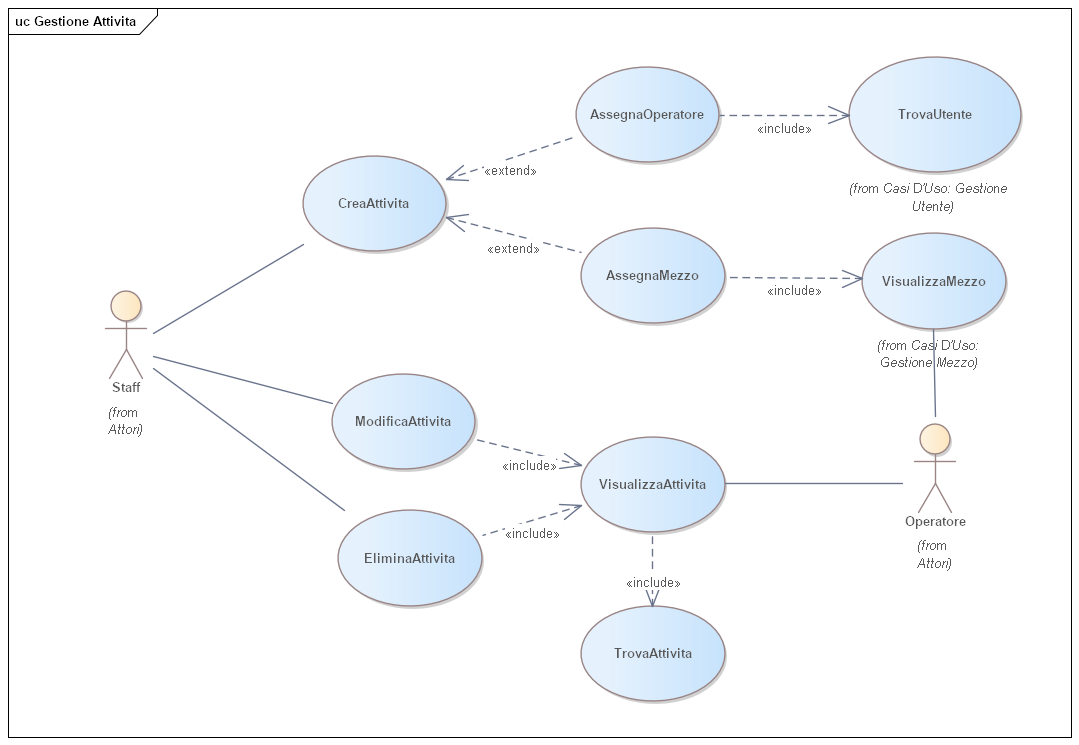
\includegraphics[width=1\textwidth]{GestioneAttivita}
\end{figure*}

% Tabelle dei casi d'uso per Gestione Attività
\clearpage
\begin{table}[H]
\vspace*{-0cm}
\renewcommand{\arraystretch}{1.9}
\begin{tabular}{|p{3.9cm}|p{9.9cm}|}
\hline
\multicolumn{2}{|c|}{\textbf{Caso d’uso: CreaAttivita}} \\ \hline
	\textbf{ID} & 19 \\ \hline
	\textbf{Breve descrizione} & Il Cliente o lo Staff crea una nuova attività di gestione dei rifiuti \\ \hline
	\textbf{Attori primari} & Cliente, Staff \\ \hline
	\textbf{Attori secondari} & Nessuno \\ \hline
	\textbf{Precondizioni} & \begin{enumerate}[leftmargin=14pt,label=\arabic*.,labelsep=0.5em,topsep=0pt,partopsep=0pt,parsep=0pt,itemsep=0pt]
    \item Il Cliente o lo Staff è autenticato
\end{enumerate} \\ \hline
	\textbf{Sequenza degli eventi principale} & \begin{enumerate}[leftmargin=14pt,label=\arabic*.,labelsep=0.5em,topsep=0pt,partopsep=0pt,parsep=0pt,itemsep=0pt]
    \item Il caso d’uso inizia quando il Cliente o lo Staff seleziona l'opzione di creazione di una nuova attività
    \item Il sistema richiede i dati dell’attività
    \item Il Cliente o lo Staff inserisce i dati
    \item \texttt{Extend} \textit{AssegnaOperatore}
    \item \texttt{Extend} \textit{AssegnaMezzo}
    \item \texttt{If} i dati sono validi
    \begin{enumerate}[label=\arabic{enumi}.\arabic*.,leftmargin=22pt,labelsep=0.5em,topsep=0pt,partopsep=0pt,parsep=0pt,itemsep=0pt]
        \item Il sistema registra la nuova attività
        \item Il sistema mostra un messaggio di conferma
    \end{enumerate}
    \item \texttt{Else}
    \begin{enumerate}[label=\arabic{enumi}.\arabic*.,leftmargin=22pt,labelsep=0.5em,topsep=0pt,partopsep=0pt,parsep=0pt,itemsep=0pt]
        \item Il sistema mostra un errore e richiede la correzione
    \end{enumerate}
\end{enumerate} \\ \hline
	\textbf{Postcondizioni} & \begin{enumerate}[label=\arabic*.,leftmargin=14pt,labelsep=0.5em,topsep=0pt,partopsep=0pt,parsep=0pt,itemsep=0pt]
        \item L’attività è creata nel sistema
    \end{enumerate} \\ \hline
	\textbf{Sequenza degli eventi alternativa} & \begin{enumerate}[leftmargin=14pt,label=\arabic*.,labelsep=0.5em,topsep=0pt,partopsep=0pt,parsep=0pt,itemsep=0pt]
    \item \texttt{If} l’operazione non è confermata
    \begin{enumerate}[label=\arabic{enumi}.\arabic*.,leftmargin=22pt,labelsep=0.5em,topsep=0pt,partopsep=0pt,parsep=0pt,itemsep=0pt]
        \item Il sistema annulla l’operazione e non apporta modifiche
    \end{enumerate}
\end{enumerate} \\ \hline
\end{tabular}
\end{table}

\clearpage
\begin{table}[H]
\vspace*{-0cm}
\renewcommand{\arraystretch}{1.9}
\begin{tabular}{|p{3.9cm}|p{9.9cm}|}
\hline
\multicolumn{2}{|c|}{\textbf{Caso d’uso: AssegnaOperatore}} \\ \hline
	\textbf{ID} & 20 \\ \hline
	\textbf{Breve descrizione} & Lo Staff assegna un Operatore ad un’attività \\ \hline
	\textbf{Attori primari} & Staff \\ \hline
	\textbf{Attori secondari} & Nessuno \\ \hline
	\textbf{Precondizioni} & \begin{enumerate}[leftmargin=14pt,label=\arabic*.,labelsep=0.5em,topsep=0pt,partopsep=0pt,parsep=0pt,itemsep=0pt]
    \item L’attività esiste
    \item L’operatore è registrato
\end{enumerate} \\ \hline
	\textbf{Sequenza degli eventi principale} & \begin{enumerate}[leftmargin=14pt,label=\arabic*.,labelsep=0.5em,topsep=0pt,partopsep=0pt,parsep=0pt,itemsep=0pt]
    \item Il caso d'uso inizia quando lo Staff seleziona l'opzione di assegnazione di un operatore all'attività
    \item \texttt{Extend} \textit{TrovaUtente}
    \item Lo Staff seleziona un operatore da assegnare all'attività
    \item \texttt{If} L’Operatore è disponibile
    \begin{enumerate}[label=\arabic{enumi}.\arabic*.,leftmargin=22pt,labelsep=0.5em,topsep=0pt,partopsep=0pt,parsep=0pt,itemsep=0pt]
        \item Il sistema registra l’assegnazione
    \end{enumerate}
    \item \texttt{Else}
    \begin{enumerate}[label=\arabic{enumi}.\arabic*.,leftmargin=22pt,labelsep=0.5em,topsep=0pt,partopsep=0pt,parsep=0pt,itemsep=0pt]
        \item Il sistema mostra il messaggio d’errore “L’operatore non è disponibile”
    \end{enumerate}
\end{enumerate} \\ \hline
	\textbf{Postcondizioni} & \begin{enumerate}[label=\arabic*.,leftmargin=14pt,labelsep=0.5em,topsep=0pt,partopsep=0pt,parsep=0pt,itemsep=0pt]
        \item L’operatore è assegnato all’attività.
    \end{enumerate} \\ \hline
	\textbf{Sequenza degli eventi alternativa} & \begin{enumerate}[leftmargin=14pt,label=\arabic*.,labelsep=0.5em,topsep=0pt,partopsep=0pt,parsep=0pt,itemsep=0pt]
    \item \texttt{If} lo Staff non conferma l’operazione
    \begin{enumerate}[label=\arabic{enumi}.\arabic*.,leftmargin=22pt,labelsep=0.5em,topsep=0pt,partopsep=0pt,parsep=0pt,itemsep=0pt]
        \item Il sistema annulla l’operazione e non apporta modifiche
    \end{enumerate}
\end{enumerate} \\ \hline
\end{tabular}
\end{table}

\clearpage
\begin{table}[H]
\vspace*{-0cm}
\renewcommand{\arraystretch}{1.9}
\begin{tabular}{|p{3.9cm}|p{9.9cm}|}
\hline
\multicolumn{2}{|c|}{\textbf{Caso d’uso: AssegnaMezzo}} \\ \hline
	\textbf{ID} & 21 \\ \hline
	\textbf{Breve descrizione} & Lo Staff assegna un mezzo ad un’attività \\ \hline
	\textbf{Attori primari} & Staff \\ \hline
	\textbf{Attori secondari} & Nessuno \\ \hline
	\textbf{Precondizioni} & \begin{enumerate}[leftmargin=14pt,label=\arabic*.,labelsep=0.5em,topsep=0pt,partopsep=0pt,parsep=0pt,itemsep=0pt]
    \item L’attività esiste
    \item Il mezzo è registrato nel sistema
\end{enumerate} \\ \hline
	\textbf{Sequenza degli eventi principale} & \begin{enumerate}[leftmargin=14pt,label=\arabic*.,labelsep=0.5em,topsep=0pt,partopsep=0pt,parsep=0pt,itemsep=0pt]
    \item Il caso d'uso inizia quando lo Staff seleziona l'opzione di assegnazione di un mezzo all'attività
    \item \texttt{Extend} \textit{TrovaMezzo}
    \item Lo Staff seleziona un mezzo da assegnare all’attività
    \item \texttt{If} Il mezzo è disponibile
    \begin{enumerate}[label=\arabic{enumi}.\arabic*.,leftmargin=22pt,labelsep=0.5em,topsep=0pt,partopsep=0pt,parsep=0pt,itemsep=0pt]
        \item Il sistema registra l’assegnazione
    \end{enumerate}
    \item \texttt{Else}
    \begin{enumerate}[label=\arabic{enumi}.\arabic*.,leftmargin=22pt,labelsep=0.5em,topsep=0pt,partopsep=0pt,parsep=0pt,itemsep=0pt]
        \item Il sistema mostra il messaggio d’errore “Il mezzo non è disponibile”
    \end{enumerate}
\end{enumerate} \\ \hline
	\textbf{Postcondizioni} & \begin{enumerate}[label=\arabic*.,leftmargin=14pt,labelsep=0.5em,topsep=0pt,partopsep=0pt,parsep=0pt,itemsep=0pt]
        \item Il mezzo è associato all’attività
    \end{enumerate} \\ \hline
	\textbf{Sequenza degli eventi alternativa} & \begin{enumerate}[leftmargin=14pt,label=\arabic*.,labelsep=0.5em,topsep=0pt,partopsep=0pt,parsep=0pt,itemsep=0pt]
    \item \texttt{If} lo Staff non conferma l’operazione
    \begin{enumerate}[label=\arabic{enumi}.\arabic*.,leftmargin=22pt,labelsep=0.5em,topsep=0pt,partopsep=0pt,parsep=0pt,itemsep=0pt]
        \item Il sistema annulla l’operazione e non apporta modifiche
    \end{enumerate}
\end{enumerate} \\ \hline
\end{tabular}
\end{table}

\clearpage
\begin{table}[H]
\vspace*{-0cm}
\renewcommand{\arraystretch}{1.9}
\begin{tabular}{|p{3.9cm}|p{9.9cm}|}
\hline
\multicolumn{2}{|c|}{\textbf{Caso d’uso: VisualizzaAttivita}} \\ \hline
	\textbf{ID} & 22 \\ \hline
	\textbf{Breve descrizione} & Il Cliente o lo Staff visualizza l’attività selezionata \\ \hline
	\textbf{Attori primari} & Cliente, Staff \\ \hline
	\textbf{Attori secondari} & Nessuno \\ \hline
	\textbf{Precondizioni} & \begin{enumerate}[leftmargin=14pt,label=\arabic*.,labelsep=0.5em,topsep=0pt,partopsep=0pt,parsep=0pt,itemsep=0pt]
    \item Il Cliente o lo Staff è autenticato
\end{enumerate} \\ \hline
	\textbf{Sequenza degli eventi principale} & \begin{enumerate}[leftmargin=14pt,label=\arabic*.,labelsep=0.5em,topsep=0pt,partopsep=0pt,parsep=0pt,itemsep=0pt]
    \item Il caso d’uso inizia quando il Cliente o lo Staff seleziona l’opzione di visualizzazione  dell'attività
    \item \texttt{Extend} \textit{TrovaAttivita}
    \item Lo Staff seleziona un’attività da visualizzare
    \item Il sistema mostra le informazioni sull’attività selezionata
\end{enumerate} \\ \hline
	\textbf{Postcondizioni} & Nessuna. \\ \hline
	\textbf{Sequenza degli eventi alternativa} & Nessuna. \\ \hline
\end{tabular}
\end{table}

\clearpage
\begin{table}[H]
\vspace*{-0cm}
\renewcommand{\arraystretch}{1.9}
\begin{tabular}{|p{3.9cm}|p{9.9cm}|}
\hline
\multicolumn{2}{|c|}{\textbf{Caso d’uso: TrovaAttivita}} \\ \hline
	\textbf{ID} & 23 \\ \hline
	\textbf{Breve descrizione} & Il Cliente o lo Staff cerca un’attività \\ \hline
	\textbf{Attori primari} & Cliente, Staff \\ \hline
	\textbf{Attori secondari} & Nessuno \\ \hline
	\textbf{Precondizioni} & \begin{enumerate}[leftmargin=14pt,label=\arabic*.,labelsep=0.5em,topsep=0pt,partopsep=0pt,parsep=0pt,itemsep=0pt]
    \item Il Cliente o lo Staff è autenticato
\end{enumerate} \\ \hline
	\textbf{Sequenza degli eventi principale} & \begin{enumerate}[leftmargin=14pt,label=\arabic*.,labelsep=0.5em,topsep=0pt,partopsep=0pt,parsep=0pt,itemsep=0pt]
    \item Il caso d’uso inizia quando il Cliente o lo Staff inserisce il singolo critero di ricerca nella barra dedicata (es. ID attività, nome)
    \item Il sistema esegue la ricerca
    \item \texttt{If} l’attività esiste
    \begin{enumerate}[label=\arabic{enumi}.\arabic*.,leftmargin=22pt,labelsep=0.5em,topsep=0pt,partopsep=0pt,parsep=0pt,itemsep=0pt]
        \item \texttt{For Each} attività trovata
        \begin{enumerate}[label=\arabic{enumi}.\arabic{enumii}.\arabic*.,leftmargin=22pt,labelsep=0.5em,topsep=0pt,partopsep=0pt,parsep=0pt,itemsep=0pt]
            \item Il sistema mostra i risultati dell'attività
        \end{enumerate}
    \end{enumerate}
    \item \texttt{Else}
    \begin{enumerate}[label=\arabic{enumi}.\arabic*.,leftmargin=22pt,labelsep=0.5em,topsep=0pt,partopsep=0pt,parsep=0pt,itemsep=0pt]
        \item Il sistema mostra “Nessuna attività trovata”
    \end{enumerate}
\end{enumerate} \\ \hline
	\textbf{Postcondizioni} & Nessuna. \\ \hline
	\textbf{Sequenza degli eventi alternativa} & Nessuna. \\ \hline
\end{tabular}
\end{table}

\clearpage
\begin{table}[H]
\vspace*{-0cm}
\renewcommand{\arraystretch}{1.9}
\begin{tabular}{|p{3.9cm}|p{9.9cm}|}
\hline
\multicolumn{2}{|c|}{\textbf{Caso d’uso: ModificaAttivita}} \\ \hline
	\textbf{ID} & 24 \\ \hline
	\textbf{Breve descrizione} & Il Cliente o lo Staff modifica un’attività esistente \\ \hline
	\textbf{Attori primari} & Cliente, Staff \\ \hline
	\textbf{Attori secondari} & Nessuno \\ \hline
	\textbf{Precondizioni} & \begin{enumerate}[leftmargin=14pt,label=\arabic*.,labelsep=0.5em,topsep=0pt,partopsep=0pt,parsep=0pt,itemsep=0pt]
    \item Il Cliente o lo Staff è autenticato
    \item L’attività esiste
\end{enumerate} \\ \hline
	\textbf{Sequenza degli eventi principale} & \begin{enumerate}[leftmargin=14pt,label=\arabic*.,labelsep=0.5em,topsep=0pt,partopsep=0pt,parsep=0pt,itemsep=0pt]
    \item Il caso d'uso inizia quando il Cliente o lo Staff seleziona l'opzione di modifica dell'attività
    \item Lo Staff aggiorna i dati dell’attività
    \item \texttt{If} i dati sono validi
    \begin{enumerate}[label=\arabic{enumi}.\arabic*.,leftmargin=22pt,labelsep=0.5em,topsep=0pt,partopsep=0pt,parsep=0pt,itemsep=0pt]
        \item Il sistema registra le modifiche
        \item \texttt{Include} \textit{(VisualizzaAttivita)}
    \end{enumerate}
    \item \texttt{Else}
    \begin{enumerate}[label=\arabic{enumi}.\arabic*.,leftmargin=22pt,labelsep=0.5em,topsep=0pt,partopsep=0pt,parsep=0pt,itemsep=0pt]
        \item Il sistema mostra un messaggio di errore
    \end{enumerate}
\end{enumerate} \\ \hline
	\textbf{Postcondizioni} & \begin{enumerate}[label=\arabic*.,leftmargin=14pt,labelsep=0.5em,topsep=0pt,partopsep=0pt,parsep=0pt,itemsep=0pt]
        \item L’attività è aggiornata nel sistema
    \end{enumerate} \\ \hline
	\textbf{Sequenza degli eventi alternativa} & \begin{enumerate}[leftmargin=14pt,label=\arabic*.,labelsep=0.5em,topsep=0pt,partopsep=0pt,parsep=0pt,itemsep=0pt]
    \item \texttt{If} l'operazione non è confermata
    \begin{enumerate}[label=\arabic{enumi}.\arabic*.,leftmargin=22pt,labelsep=0.5em,topsep=0pt,partopsep=0pt,parsep=0pt,itemsep=0pt]
        \item Il sistema annulla l’operazione e non apporta modifiche
    \end{enumerate}
\end{enumerate} \\ \hline
\end{tabular}
\end{table}

\clearpage
\begin{table}[H]
\vspace*{-0cm}
\renewcommand{\arraystretch}{1.9}
\begin{tabular}{|p{3.9cm}|p{9.9cm}|}
\hline
\multicolumn{2}{|c|}{\textbf{Caso d’uso: EliminaAttivita}} \\ \hline
	\textbf{ID} & 25 \\ \hline
	\textbf{Breve descrizione} & Il Cliente o lo Staff elimina un’attività esistente \\ \hline
	\textbf{Attori primari} & Cliente, Staff \\ \hline
	\textbf{Attori secondari} & Nessuno \\ \hline
	\textbf{Precondizioni} & \begin{enumerate}[leftmargin=14pt,label=\arabic*.,labelsep=0.5em,topsep=0pt,partopsep=0pt,parsep=0pt,itemsep=0pt]
    \item Il Cliente o lo Staff è autenticato
    \item L’attività esiste
\end{enumerate} \\ \hline
	\textbf{Sequenza degli eventi principale} & \begin{enumerate}[leftmargin=14pt,label=\arabic*.,labelsep=0.5em,topsep=0pt,partopsep=0pt,parsep=0pt,itemsep=0pt]
    \item Il caso d'uso inizia quando il Cliente o lo Staff seleziona l'opzione di eliminazione dell'attività
    \item Il Cliente o lo Staff seleziona l'attività da eliminare
    \item Il sistema elimina l’attività selezionata
\end{enumerate} \\ \hline
	\textbf{Postcondizioni} & \begin{enumerate}[label=\arabic*.,leftmargin=14pt,labelsep=0.5em,topsep=0pt,partopsep=0pt,parsep=0pt,itemsep=0pt]
        \item L’attività è eliminata
    \end{enumerate} \\ \hline
	\textbf{Sequenza degli eventi alternativa} & \begin{enumerate}[leftmargin=14pt,label=\arabic*.,labelsep=0.5em,topsep=0pt,partopsep=0pt,parsep=0pt,itemsep=0pt]
    \item \texttt{If} l'operazione non è confermata
    \begin{enumerate}[label=\arabic{enumi}.\arabic*.,leftmargin=22pt,labelsep=0.5em,topsep=0pt,partopsep=0pt,parsep=0pt,itemsep=0pt]
        \item Il sistema annulla l’operazione e non apporta modifiche
    \end{enumerate}
\end{enumerate} \\ \hline
\end{tabular}
\end{table}

\clearpage

\newsubsection*{Gestione Documento}

Il diagramma evidenzia le relazioni tra attori e casi d’uso relativi alla creazione, gestione e notifica dei documenti (es. FIR, scadenze, rinnovi).

\begin{figure*}[ht]
    \centering
    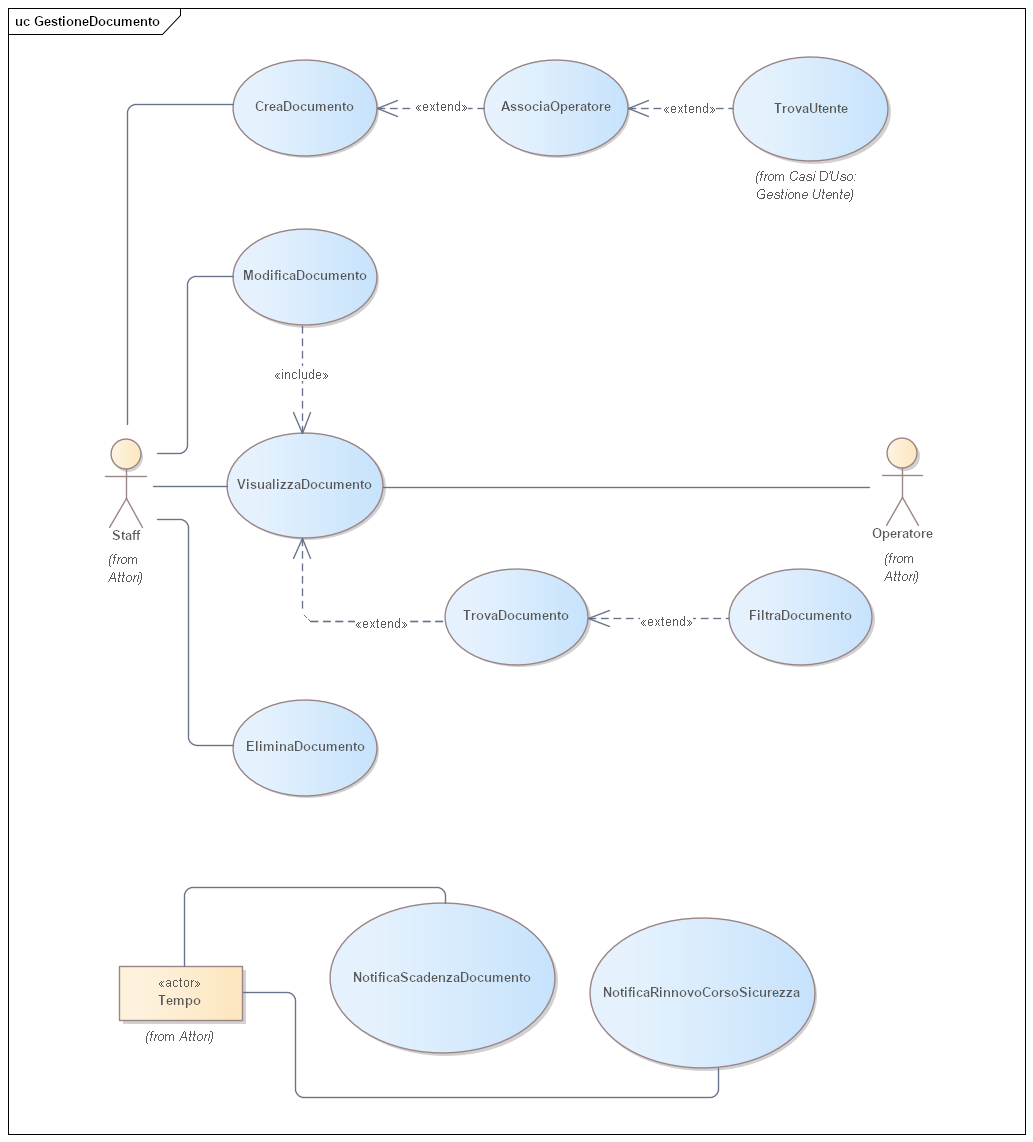
\includegraphics[width=1\textwidth]{GestioneDocumento}
\end{figure*}

\clearpage
\renewcommand{\arraystretch}{1.9}
\begin{table}[H]
\vspace*{-0cm}
\begin{tabular}{|p{3.9cm}|p{9.9cm}|}
\hline
\multicolumn{2}{|c|}{\textbf{Caso d’uso: CreaDocumento}} \\ \hline
	\textbf{ID} & 26 \\ \hline
	\textbf{Breve descrizione} & Lo Staff crea un nuovo documento nel sistema \\ \hline
	\textbf{Attori primari} & Staff \\ \hline
	\textbf{Attori secondari} & Nessuno \\ \hline
	\textbf{Precondizioni} & \begin{enumerate}[leftmargin=14pt,label=\arabic*.,labelsep=0.5em,topsep=0pt,partopsep=0pt,parsep=0pt,itemsep=0pt]
        \item Lo Staff è stato autenticato dal sistema
    \end{enumerate} \\ \hline
	\textbf{Sequenza degli eventi principale} &
\begin{enumerate}[leftmargin=14pt,label=\arabic*.,labelsep=0.5em,topsep=0pt,partopsep=0pt,parsep=0pt,itemsep=0pt]
    \item Il caso d’uso inizia quando lo Staff seleziona l'opzione di creazione del documento
    \item Il sistema richiede i dati del documento
    \item Lo Staff inserisce i dati
    \item \texttt{If} i dati sono validi e non duplicati
    \begin{enumerate}[label=\arabic{enumi}.\arabic*.,leftmargin=22pt,labelsep=0.5em,topsep=0pt,partopsep=0pt,parsep=0pt,itemsep=0pt]
        \item Il sistema registra il documento
    \end{enumerate}
    \item \texttt{Else}
    \begin{enumerate}[label=\arabic{enumi}.\arabic*.,leftmargin=22pt,labelsep=0.5em,topsep=0pt,partopsep=0pt,parsep=0pt,itemsep=0pt]
        \item Il sistema segnala un errore e richiede la correzione
    \end{enumerate}
\end{enumerate}\\ \hline
	\textbf{Postcondizioni} & \begin{enumerate}[label=\arabic*.,leftmargin=14pt,labelsep=0.5em,topsep=0pt,partopsep=0pt,parsep=0pt,itemsep=0pt]
        \item Il documento è registrato nel sistema
    \end{enumerate} \\ \hline
	\textbf{Sequenza degli eventi alternativa} & 
\begin{enumerate}[leftmargin=14pt,label=\arabic*.,labelsep=0.5em,topsep=0pt,partopsep=0pt,parsep=0pt,itemsep=0pt]
    \item \texttt{If} lo Staff non conferma l’operazione
    \begin{enumerate}[label=\arabic{enumi}.\arabic*.,leftmargin=22pt,labelsep=0.5em,topsep=0pt,partopsep=0pt,parsep=0pt,itemsep=0pt]
        \item Il sistema annulla l’operazione e nessun documento viene creato
    \end{enumerate}
\end{enumerate} \\ \hline
\end{tabular}
\end{table}

\clearpage
\begin{table}[H]
\vspace*{-0cm}
\renewcommand{\arraystretch}{1.9}
\begin{tabular}{|p{3.9cm}|p{9.9cm}|}
\hline
\multicolumn{2}{|c|}{\textbf{Caso d’uso: VisualizzaDocumento}} \\ \hline
	\textbf{ID} & 27 \\ \hline
	\textbf{Breve descrizione} & L’Operatore visualizza i dati di un documento \\ \hline
	\textbf{Attori primari} & Operatore \\ \hline
	\textbf{Attori secondari} & Nessuno \\ \hline
	\textbf{Precondizioni} & \begin{enumerate}[leftmargin=14pt,label=\arabic*.,labelsep=0.5em,topsep=0pt,partopsep=0pt,parsep=0pt,itemsep=0pt]
        \item Operatore è autenticato
        \item Il documento esiste
    \end{enumerate} \\ \hline
	\textbf{Sequenza degli eventi principale} &
    \begin{enumerate}[leftmargin=14pt,label=\arabic*.,labelsep=0.5em,topsep=0pt,partopsep=0pt,parsep=0pt,itemsep=0pt]
        \item Il caso d’uso inizia quando l’Operatore seleziona l'opzione di visualizzazione del documento
        \item \texttt{Extend} \textit{TrovaDocumento}
        \item L'Operatore seleziona un documento
        \item Il sistema mostra i dati del documento selezionato
    \end{enumerate} \\ \hline
	\textbf{Postcondizioni} & Nessuna \\ \hline
	\textbf{Sequenza degli eventi alternativa} & Nessuna \\ \hline
\end{tabular}
\end{table}

\clearpage
\begin{table}[H]
\vspace*{-0cm}
\renewcommand{\arraystretch}{1.9}
\begin{tabular}{|p{3.9cm}|p{9.9cm}|}
\hline
\multicolumn{2}{|c|}{\textbf{Caso d’uso: TrovaDocumento}} \\ \hline
	\textbf{ID} & 28 \\ \hline
	\textbf{Breve descrizione} & L’Operatore ricerca uno o più documenti \\ \hline
	\textbf{Attori primari} & Operatore \\ \hline
	\textbf{Attori secondari} & Nessuno \\ \hline
	\textbf{Precondizioni} & \begin{enumerate}[leftmargin=14pt,label=\arabic*.,labelsep=0.5em,topsep=0pt,partopsep=0pt,parsep=0pt,itemsep=0pt]
        \item L’Operatore è autenticato.
    \end{enumerate} \\ \hline
	\textbf{Sequenza degli eventi principale} & 
\begin{enumerate}[leftmargin=14pt,label=\arabic*.,labelsep=0.5em,topsep=0pt,partopsep=0pt,parsep=0pt,itemsep=0pt]
    \item Il caso d’uso inizia quando l’Operatore inserisce il singolo criterio di ricerca nella barra dedicata (es. ID documento, nome)
    \item \texttt{Extend} \textit{FiltraDocumento}
    \item \texttt{If} il documento esiste
    \begin{enumerate}[label=\arabic{enumi}.\arabic*.,leftmargin=22pt,labelsep=0.5em,topsep=0pt,partopsep=0pt,parsep=0pt,itemsep=0pt]
        \item \texttt{For Each} documento trovato
        \begin{enumerate}[label=\arabic{enumi}.\arabic{enumii}.\arabic*.,leftmargin=22pt,labelsep=0.5em,topsep=0pt,partopsep=0pt,parsep=0pt,itemsep=0pt]
            \item Il sistema mostra le informazioni base del documento (es. ID, nome, ecc.)
        \end{enumerate}
    \end{enumerate}
    \item \texttt{Else}
    \begin{enumerate}[label=\arabic{enumi}.\arabic*.,leftmargin=22pt,labelsep=0.5em,topsep=0pt,partopsep=0pt,parsep=0pt,itemsep=0pt]
        \item Il sistema mostra “Nessun documento trovato”
    \end{enumerate}
\end{enumerate}\\ \hline
	\textbf{Postcondizioni} & Nessuna \\ \hline
	\textbf{Sequenza degli eventi alternativa} & Nessuna \\ \hline
\end{tabular}
\end{table}

\clearpage
\begin{table}[H]
\vspace*{-0cm}
\renewcommand{\arraystretch}{1.9}
\begin{tabular}{|p{3.9cm}|p{9.9cm}|}
\hline
\multicolumn{2}{|c|}{\textbf{Caso d’uso: FiltraDocumento}} \\ \hline
	\textbf{ID} & 29 \\ \hline
	\textbf{Breve descrizione} & L'Operatore filtra i documenti in base a criteri avanzati (tipo, data di creazione, ecc.)  \\ \hline
	\textbf{Attori primari} & Operatore  \\ \hline
	\textbf{Attori secondari} & Nessuno \\ \hline
	\textbf{Precondizioni} & \begin{enumerate}[leftmargin=14pt,label=\arabic*.,labelsep=0.5em,topsep=0pt,partopsep=0pt,parsep=0pt,itemsep=0pt]
        \item L’Operatore è autenticato
    \end{enumerate} \\ \hline
	\textbf{Sequenza degli eventi principale} & 
\begin{enumerate}[leftmargin=14pt,label=\arabic*.,labelsep=0.5em,topsep=0pt,partopsep=0pt,parsep=0pt,itemsep=0pt]
    \item Il caso d’uso inizia quando l’Operatore applica filtri avanzati
    \item \texttt{If} esistono documenti che rispettano i filtri
    \begin{enumerate}[label=\arabic{enumi}.\arabic*.,leftmargin=22pt,labelsep=0.5em,topsep=0pt,partopsep=0pt,parsep=0pt,itemsep=0pt]
        \item Il sistema mostra l'elenco dei documenti filtrati
    \end{enumerate}
    \item \texttt{Else}
    \begin{enumerate}[label=\arabic{enumi}.\arabic*.,leftmargin=22pt,labelsep=0.5em,topsep=0pt,partopsep=0pt,parsep=0pt,itemsep=0pt]
        \item Il sistema mostra “Nessun documento corrisponde ai criteri di filtro”
    \end{enumerate}
\end{enumerate}\\ \hline
	\textbf{Postcondizioni} & \begin{enumerate}[label=\arabic*.,leftmargin=14pt,labelsep=0.5em,topsep=0pt,partopsep=0pt,parsep=0pt,itemsep=0pt]
        \item L’Operatore visualizza i documenti filtrati
    \end{enumerate} \\ \hline
	\textbf{Sequenza degli eventi alternativa} & Nessuna \\ \hline
\end{tabular}
\end{table}

\clearpage
\begin{table}[H]
\vspace*{-0cm}
\renewcommand{\arraystretch}{1.9}
\begin{tabular}{|p{3.9cm}|p{9.9cm}|}
\hline
\multicolumn{2}{|c|}{\textbf{Caso d’uso: ModificaDocumento}} \\ \hline
	\textbf{ID} & 30 \\ \hline
	\textbf{Breve descrizione} & Lo Staff modifica i dati di un documento esistente \\ \hline
	\textbf{Attori primari} & Staff \\ \hline
	\textbf{Attori secondari} & Nessuno \\ \hline
	\textbf{Precondizioni} & \begin{enumerate}[leftmargin=14pt,label=\arabic*.,labelsep=0.5em,topsep=0pt,partopsep=0pt,parsep=0pt,itemsep=0pt]
        \item Lo Staff è autenticato
        \item Il documento esiste
    \end{enumerate} \\ \hline
	\textbf{Sequenza degli eventi principale} & 
    \begin{enumerate}[leftmargin=14pt,label=\arabic*.,labelsep=0.5em,topsep=0pt,partopsep=0pt,parsep=0pt,itemsep=0pt]
        \item Il caso d’uso inizia quando lo Staff seleziona l'opzione di modifica del documento
        \item Lo Staff modifica i dati del documento
        \item \texttt{If} i dati modificati sono validi
        \begin{enumerate}[label=\arabic{enumi}.\arabic*.,leftmargin=22pt,labelsep=0.5em,topsep=0pt,partopsep=0pt,parsep=0pt,itemsep=0pt]
            \item Il sistema aggiorna il documento
            \item \texttt{Include} \textit{(VisualizzaDocumento)}
        \end{enumerate}
        \item \texttt{Else}
        \begin{enumerate}[label=\arabic{enumi}.\arabic*.,leftmargin=22pt,labelsep=0.5em,topsep=0pt,partopsep=0pt,parsep=0pt,itemsep=0pt]
            \item Il sistema mostra un messaggio di errore
        \end{enumerate}
    \end{enumerate}\\ \hline
	\textbf{Postcondizioni} & 
    \begin{enumerate}[leftmargin=14pt,label=\arabic*.,labelsep=0.5em,topsep=0pt,partopsep=0pt,parsep=0pt,itemsep=0pt]
        \item I dati del documento risultano aggiornati \end{enumerate} \\ \hline
	\textbf{Sequenza degli eventi alternativa} & 
\begin{enumerate}[leftmargin=14pt,label=\arabic*.,labelsep=0.5em,topsep=0pt,partopsep=0pt,parsep=0pt,itemsep=0pt]
    \item \texttt{If} lo Staff non conferma l’operazione
    \begin{enumerate}[label=\arabic{enumi}.\arabic*.,leftmargin=22pt,labelsep=0.5em,topsep=0pt,partopsep=0pt,parsep=0pt,itemsep=0pt]
        \item Il sistema annulla l’operazione e il documento non viene modificato
    \end{enumerate}
\end{enumerate} \\ \hline
\end{tabular}
\end{table}

\clearpage
\begin{table}[H]
\vspace*{-0cm}
\renewcommand{\arraystretch}{1.9}
\begin{tabular}{|p{3.9cm}|p{9.9cm}|}
\hline
\multicolumn{2}{|c|}{\textbf{Caso d’uso: EliminaDocumento}} \\ \hline
	\textbf{ID} & 31 \\ \hline
	\textbf{Breve descrizione} & Lo Staff elimina un documento dal sistema \\ \hline
	\textbf{Attori primari} & Staff \\ \hline
	\textbf{Attori secondari} & Nessuno \\ \hline
	\textbf{Precondizioni} & \begin{enumerate}[leftmargin=14pt,label=\arabic*.,labelsep=0.5em,topsep=0pt,partopsep=0pt,parsep=0pt,itemsep=0pt]
        \item Lo Staff è autenticato
        \item Il documento esiste
    \end{enumerate} \\ \hline
	\textbf{Sequenza degli eventi principale} & 
\begin{enumerate}[leftmargin=14pt,label=\arabic*.,labelsep=0.5em,topsep=0pt,partopsep=0pt,parsep=0pt,itemsep=0pt]
    \item Il caso d’uso inizia quando lo Staff seleziona l'opzione di eliminazione del documento
    \item Lo Staff seleziona il documento da eliminare
    \item Il sistema elimina il documento selezionato
\end{enumerate}\\ \hline
	\textbf{Postcondizioni} & \begin{enumerate}[leftmargin=14pt,label=\arabic*.,labelsep=0.5em,topsep=0pt,partopsep=0pt,parsep=0pt,itemsep=0pt]
        \item Il documento è eliminato
    \end{enumerate}\\ \hline
	\textbf{Sequenza degli eventi alternativa} & 
\begin{enumerate}[leftmargin=14pt,label=\arabic*.,labelsep=0.5em,topsep=0pt,partopsep=0pt,parsep=0pt,itemsep=0pt]
    \item \texttt{If} lo Staff non conferma l’operazione
    \begin{enumerate}[label=\arabic{enumi}.\arabic*.,leftmargin=22pt,labelsep=0.5em,topsep=0pt,partopsep=0pt,parsep=0pt,itemsep=0pt]
        \item Il sistema annulla l’operazione e il documento viene eliminato
    \end{enumerate}
\end{enumerate} \\ \hline
\end{tabular}
\end{table}

\clearpage
\begin{table}[H]
\vspace*{-0cm}
\renewcommand{\arraystretch}{1.9}
\begin{tabular}{|p{3.9cm}|p{9.9cm}|}
\hline
\multicolumn{2}{|c|}{\textbf{Caso d’uso: NotificaRinnovoCorsoSicurezza}} \\ \hline
	\textbf{ID} & 32 \\ \hline
	\textbf{Breve descrizione} & Il sistema invia le notifiche relative al rinnovo dei corsi sulla sicurezza \\ \hline
	\textbf{Attori primari} & Tempo \\ \hline
	\textbf{Attori secondari} & Nessuno \\ \hline
	\textbf{Precondizioni} & \begin{enumerate}[leftmargin=14pt,label=\arabic*.,labelsep=0.5em,topsep=0pt,partopsep=0pt,parsep=0pt,itemsep=0pt]
        \item Esistono corsi sulla sicurezza con data di scadenza registrata
    \end{enumerate} \\ \hline
	\textbf{Sequenza degli eventi principale} & 
\begin{enumerate}[leftmargin=14pt,label=\arabic*.,labelsep=0.5em,topsep=0pt,partopsep=0pt,parsep=0pt,itemsep=0pt]
    \item Il caso d’uso inizia quando al raggiungimento della data predefinita, l’attore Tempo innesca il controllo dei corsi in scadenza
    \item \texttt{For Each} corso in scadenza
    \begin{enumerate}[label=\arabic{enumi}.\arabic*.,leftmargin=22pt,labelsep=0.5em,topsep=0pt,partopsep=0pt,parsep=0pt,itemsep=0pt]
        \item Il sistema invia la notifica all’Operatore o allo Staff interessato
    \end{enumerate}
\end{enumerate}\\ \hline
	\textbf{Postcondizioni} &
    \begin{enumerate}[label=\arabic*.,leftmargin=14pt,labelsep=0.5em,topsep=0pt,partopsep=0pt,parsep=0pt,itemsep=0pt]
        \item Le notifiche di rinnovo dei corsi sulla sicurezza sono state inviate
    \end{enumerate} \\ \hline
	\textbf{Sequenza degli eventi alternativa} & Nessuna. \\ \hline
\end{tabular}
\end{table}

\clearpage
\begin{table}[H]
\vspace*{-0cm}
\renewcommand{\arraystretch}{1.9}
\begin{tabular}{|p{3.9cm}|p{9.9cm}|}
\hline
\multicolumn{2}{|c|}{\textbf{Caso d’uso: NotificaScadenzaDocumento}} \\ \hline
	\textbf{ID} & 33 \\ \hline
	\textbf{Breve descrizione} & Il sistema invia la notifica per la scadenza dei documenti (es. compilazione FIR, possibilità di eliminazione documento, ecc.) \\ \hline
	\textbf{Attori primari} & Tempo \\ \hline
	\textbf{Attori secondari} & Nessuno \\ \hline
	\textbf{Precondizioni} & \begin{enumerate}[leftmargin=14pt,label=\arabic*.,labelsep=0.5em,topsep=0pt,partopsep=0pt,parsep=0pt,itemsep=0pt]
        \item Esistono documenti con data di scadenza registrata
    \end{enumerate} \\ \hline
	\textbf{Sequenza degli eventi principale} & 
\begin{enumerate}[leftmargin=14pt,label=\arabic*.,labelsep=0.5em,topsep=0pt,partopsep=0pt,parsep=0pt,itemsep=0pt]
    \item Il caso d’uso inizia quando al raggiungimento della data predefinita, l’attore Tempo innesca il controllo dei documenti in scadenza
    \item \texttt{For Each} ogni documento in scadenza
    \begin{enumerate}[label=\arabic{enumi}.\arabic*.,leftmargin=22pt,labelsep=0.5em,topsep=0pt,partopsep=0pt,parsep=0pt,itemsep=0pt]
        \item Il sistema invia la notifica allo Staff o all’Operatore
    \end{enumerate}
\end{enumerate}\\ \hline
	\textbf{Postcondizioni} & \begin{enumerate}[label=\arabic*.,leftmargin=14pt,labelsep=0.5em,topsep=0pt,partopsep=0pt,parsep=0pt,itemsep=0pt]
        \item Le notifiche di scadenza dei documenti sono state inviate
    \end{enumerate} \\ \hline
	\textbf{Sequenza degli eventi alternativa} & Nessuna \\ \hline
\end{tabular}
\end{table}

\clearpage
\newsection{Matrice di Mapping}

\begin{figure*}[!ht]
    \centering
    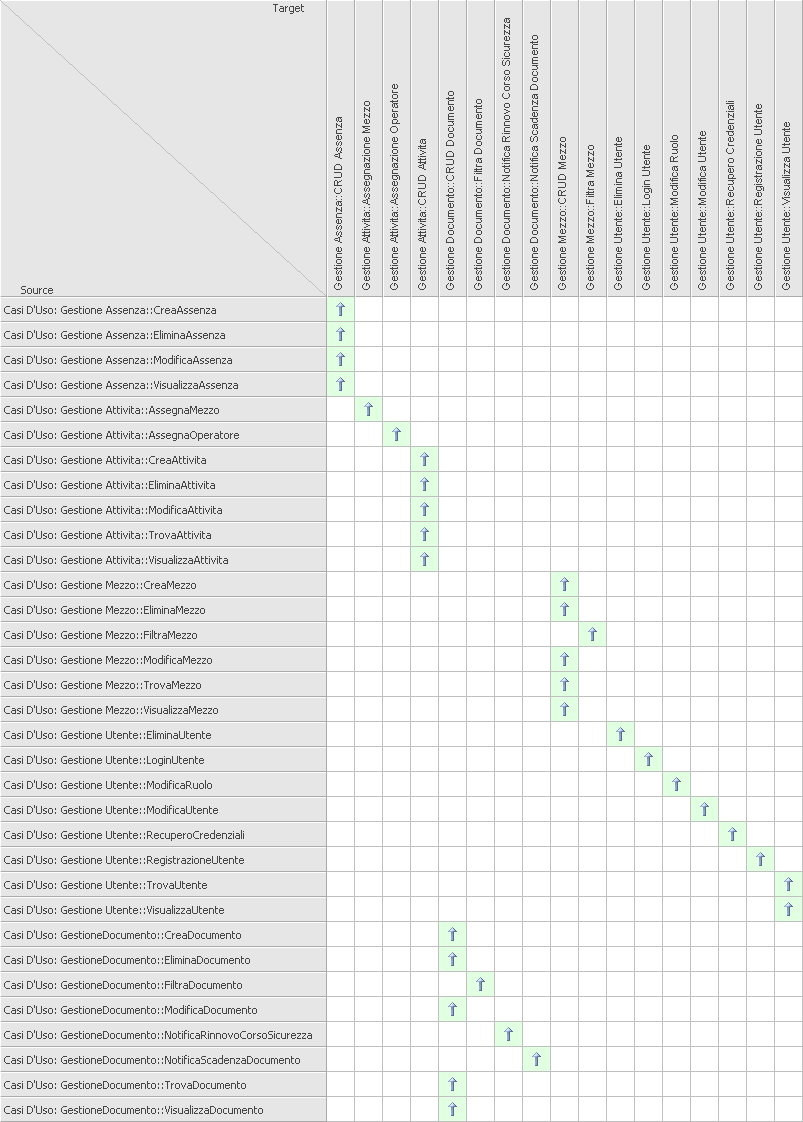
\includegraphics[width=1\textwidth]{MatriceMapping}
\end{figure*}

\newchapter{Analisi}

\newsection{Diagrammi delle Classi di Analisi}

\newsubsection{Package di Analisi}
Il diagramma mostra la struttura dei package del sistema e le dipendenze tra i moduli principali, evidenziando come le classi siano organizzate per responsabilità.

\begin{figure*}[!ht]
    \centering
    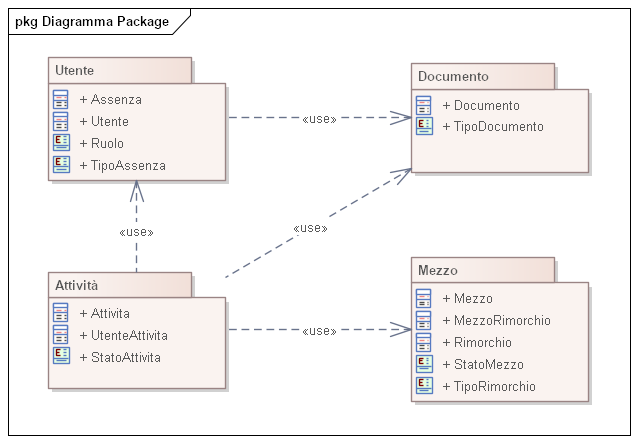
\includegraphics[width=1\textwidth]{DiagrammaPackageAnalisi}
\end{figure*}

\clearpage
\newsubsection{Classi di Analisi: Utente}
Il diagramma evidenzia le relazioni tra la classe Utente e le altre classi del sistema, mettendo in luce associazioni, dipendenze e responsabilità condivise tra i diversi ruoli.

\begin{figure*}[!ht]
    \centering
    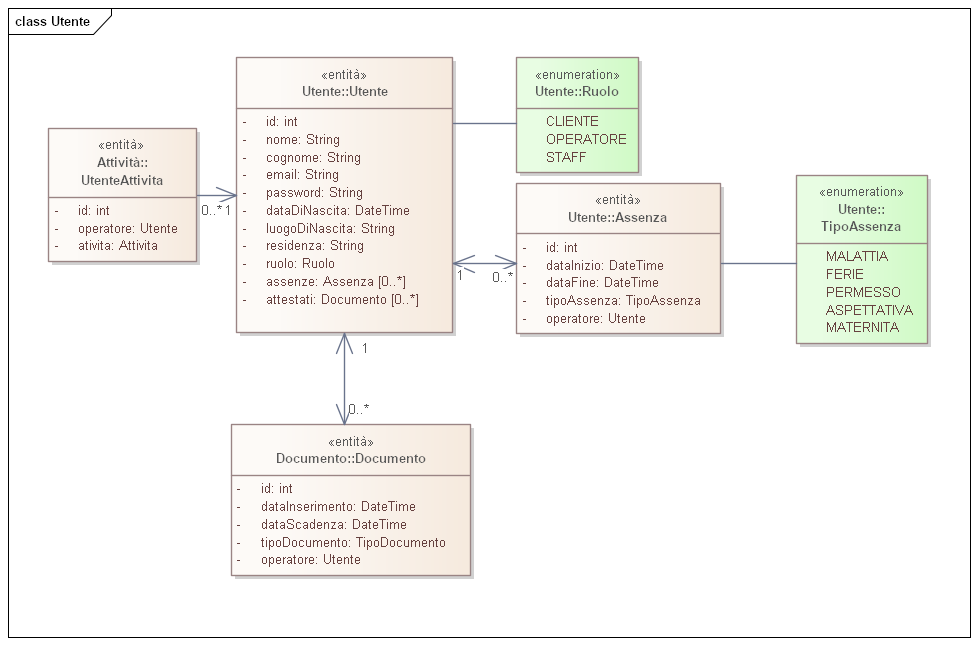
\includegraphics[width=1\textwidth]{DiagrammaClassiUtenteAnalisi}
\end{figure*}

\clearpage
\newsubsection{Classi di Analisi: Mezzo}
Il diagramma mette in evidenza le classi che modellano i mezzi, le loro proprietà e le relazioni con le attività e le informazioni di manutenzione.

\begin{figure*}[!ht]
    \centering
    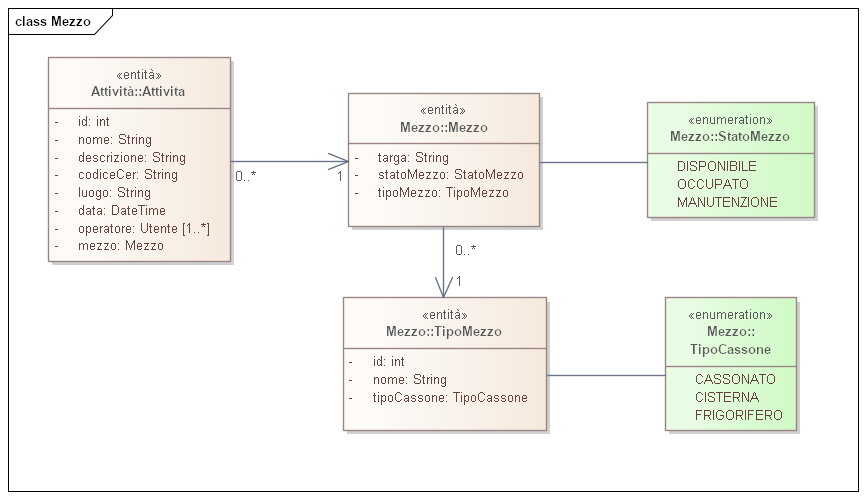
\includegraphics[width=1\textwidth]{DiagrammaClassiMezzoAnalisi}
\end{figure*}

\clearpage
\newsubsection{Classi di Analisi: Attività}
Il diagramma descrive le classi coinvolte nella gestione delle attività di carico/scarico, mostrando attributi, operazioni e collegamenti con operatori e mezzi.

\begin{figure*}[!ht]
    \centering
    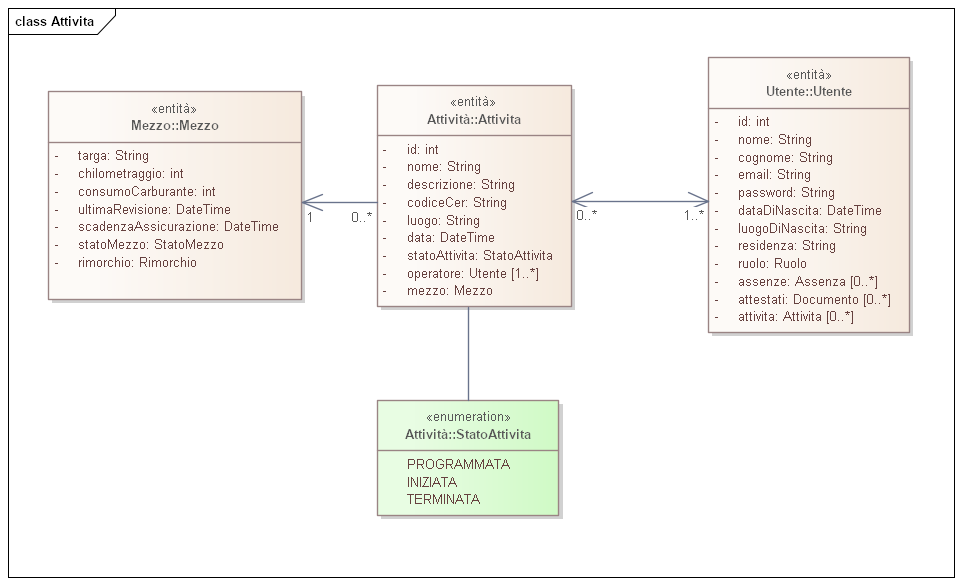
\includegraphics[width=1\textwidth]{DiagrammaClassiAttivitaAnalisi}
\end{figure*}

\clearpage
\newsubsection{Classi di Analisi: Documento}
Il diagramma illustra la struttura delle classi che rappresentano i documenti (es. FIR), con le relazioni e le responsabilità nel ciclo di vita dei documenti.

\begin{figure*}[!ht]
    \centering
    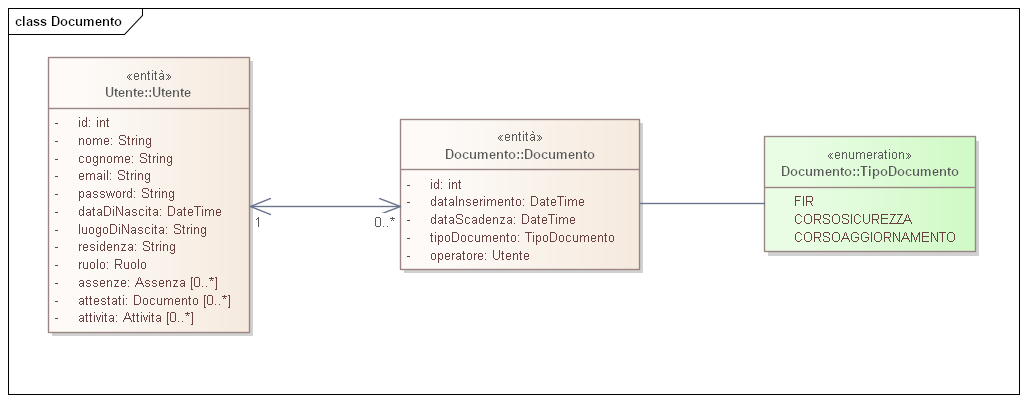
\includegraphics[width=1\textwidth]{DiagrammaClassiDocumentoAnalisi}
\end{figure*}

\clearpage
\newsection{Diagrammi di Sequenza}

\newsubsection{Login Utente}
\noindent
Il diagramma di sequenza seguente mette in evidenza il processo di accesso dell'utente al sistema: l'utente inserisce le proprie credenziali che vengono inoltrate a un servizio di autenticazione esterno per la validazione; in caso di esito positivo viene stabilita la sessione utente e l'applicazione reindirizza l'utente alla vista corrispondente al suo ruolo (ad esempio Staff, Operatore o Cliente). In caso di autenticazione fallita, il sistema restituisce un messaggio di errore e richiede un nuovo tentativo.

\begin{figure*}[!ht]
    \centering
    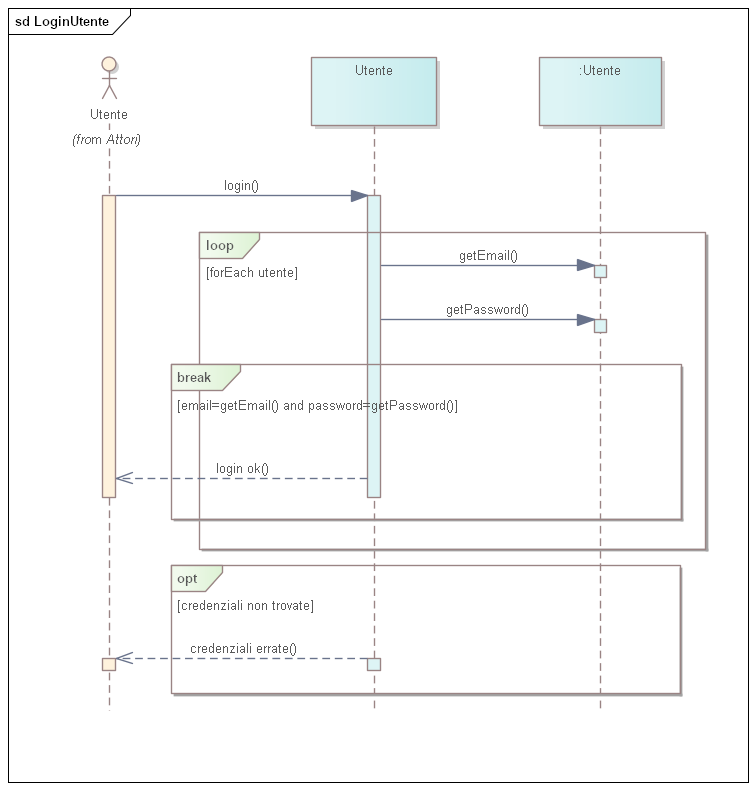
\includegraphics[width=1\textwidth]{DiagrammaSequenzaLoginUtente}
\end{figure*}

\clearpage
\newsubsection{Registrazione Utente}
\noindent
Il diagramma di sequenza mostra il processo di registrazione di un nuovo utente al sistema. Viene evidenziato il controllo sull’unicità dell’email fornita e, in caso positivo, la creazione del relativo account. In alternativa, se l’email risulta già utilizzata, il sistema restituisce un messaggio di errore.

\begin{figure*}[!ht]
    \centering
    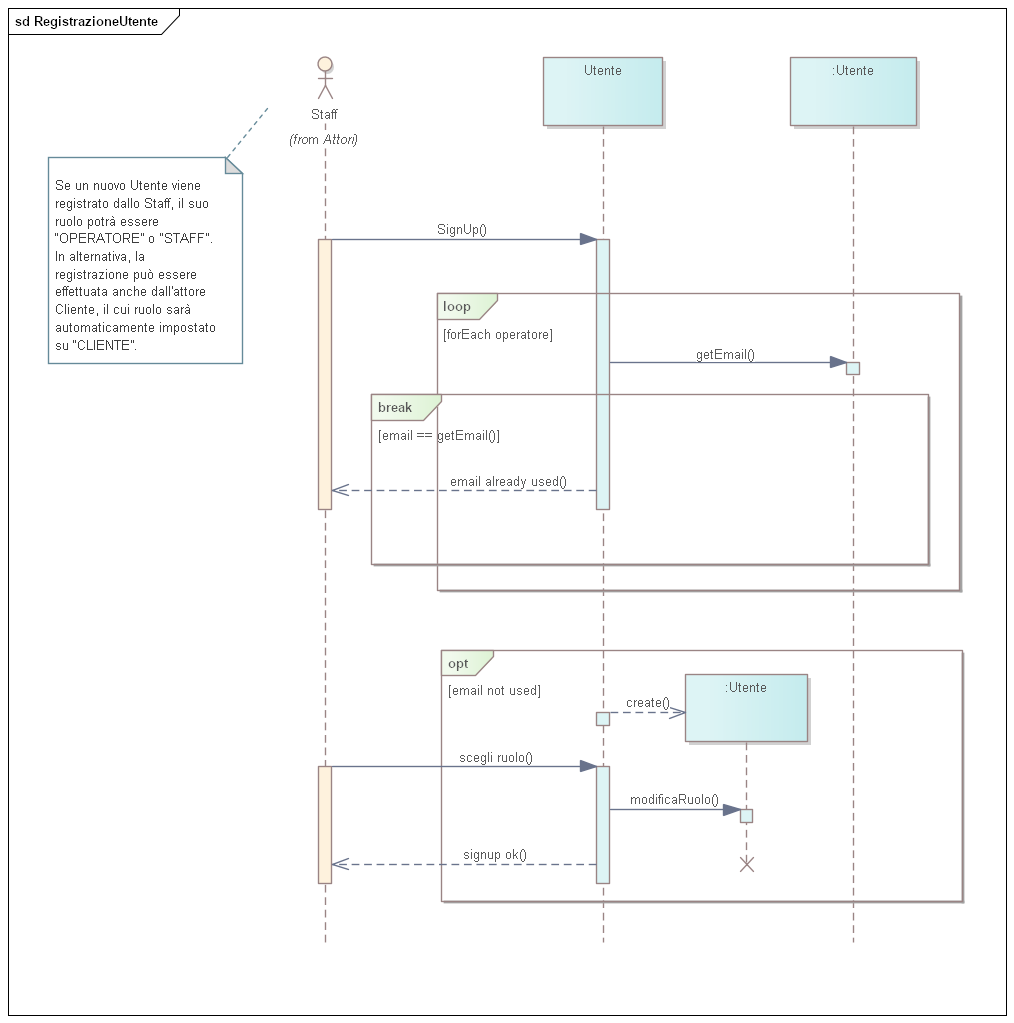
\includegraphics[width=1\textwidth]{DiagrammaSequenzaRegistrazioneUtente}
\end{figure*}

\clearpage
\newsubsection{CRUD Attività}
\noindent
Il diagramma di sequenza illustra le operazioni principali di gestione delle attività, comprendendo creazione, visualizzazione, modifica ed eliminazione. Viene rappresentato come l’attore interagisce con il sistema per svolgere ciascuna di queste funzioni, con il sistema che valida i dati e aggiorna le informazioni in modo coerente.

\begin{figure}[!ht]
  \centering
  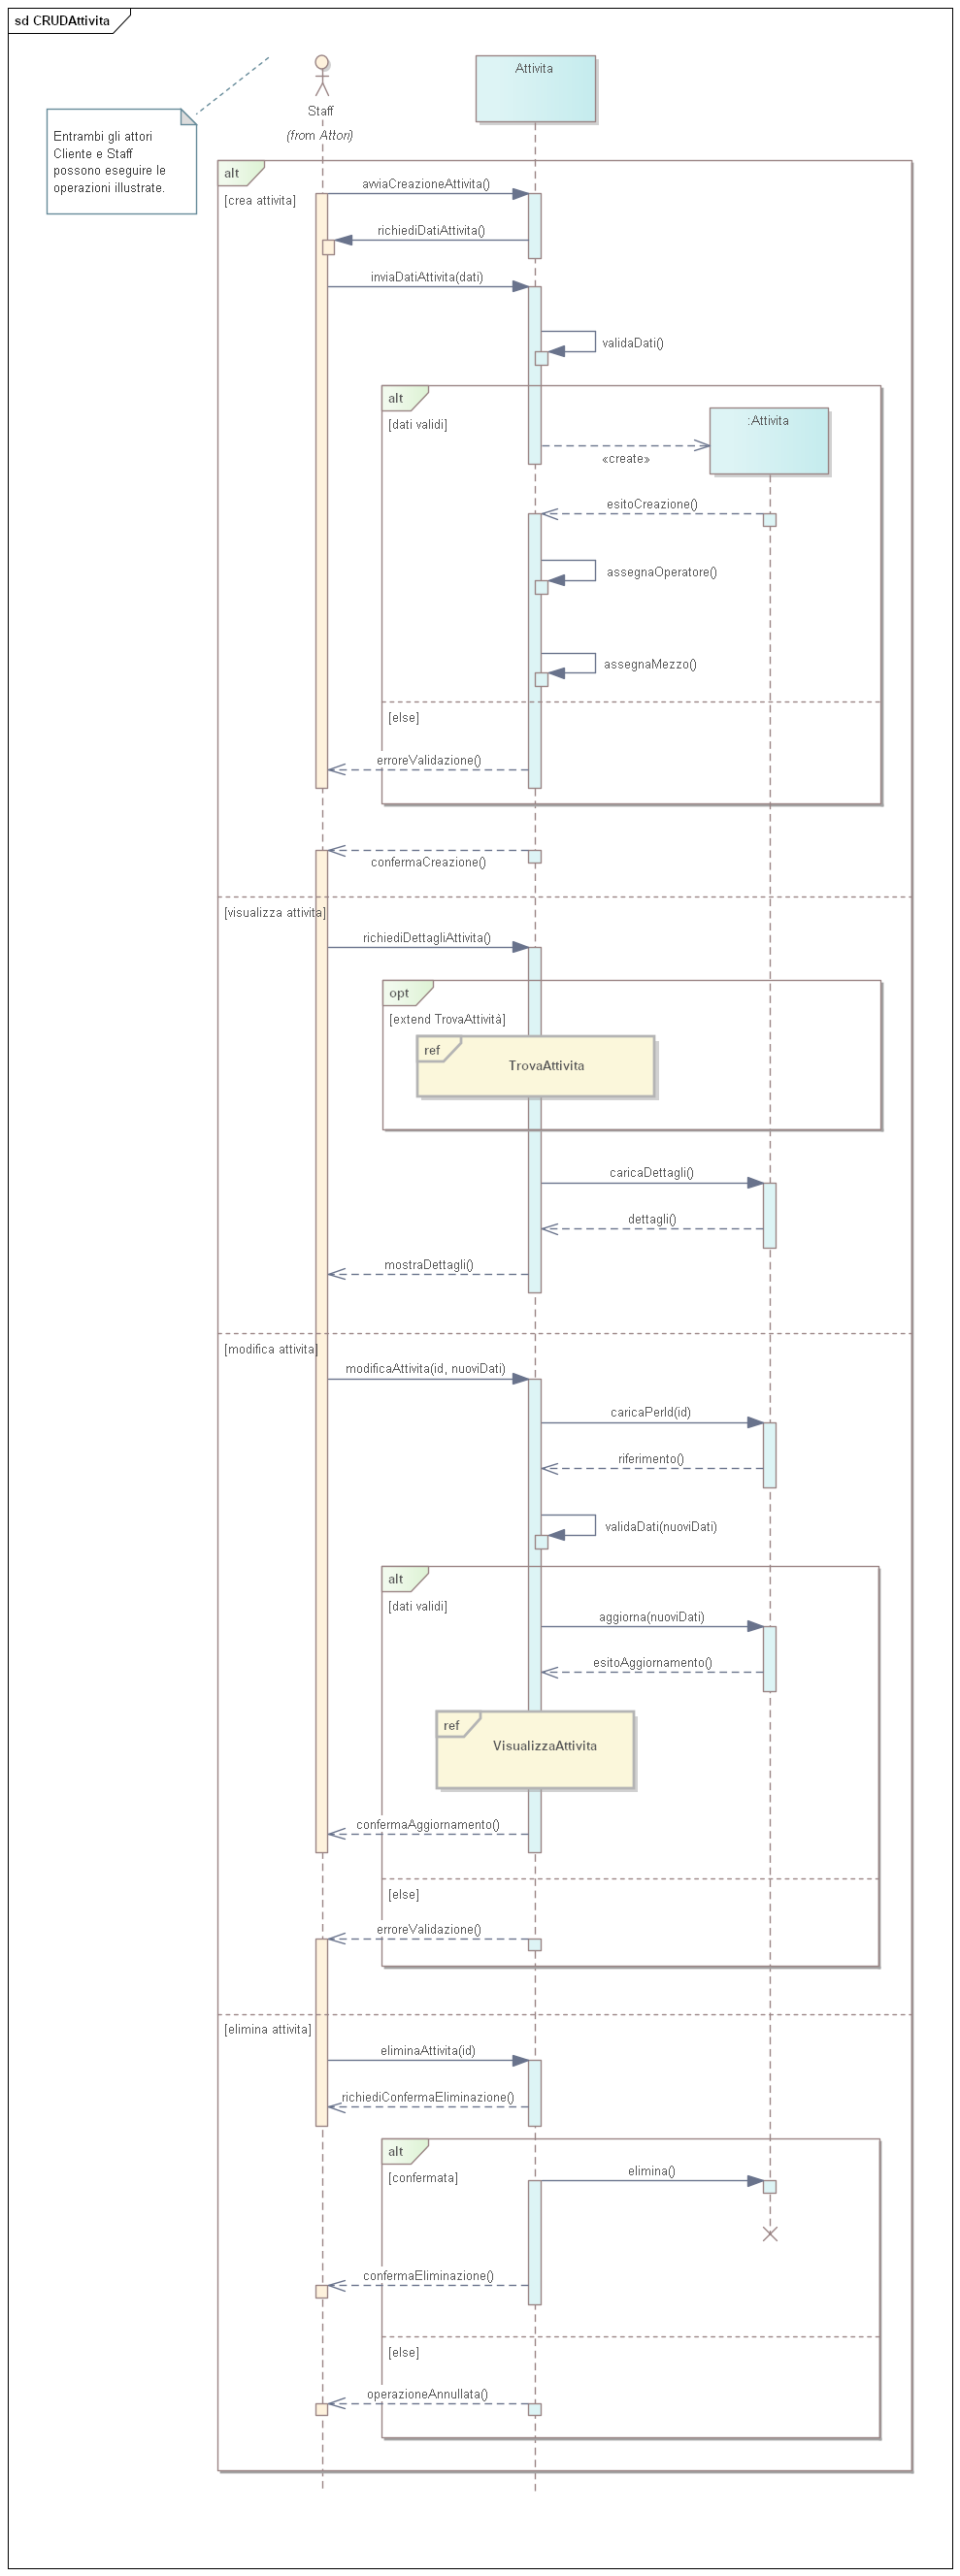
\includegraphics[width=\textwidth,trim=0 730pt 0 0,clip]{DiagrammaSequenzaCRUDAttivita}
\end{figure}
\clearpage
\begin{figure}[!ht]
  \centering
  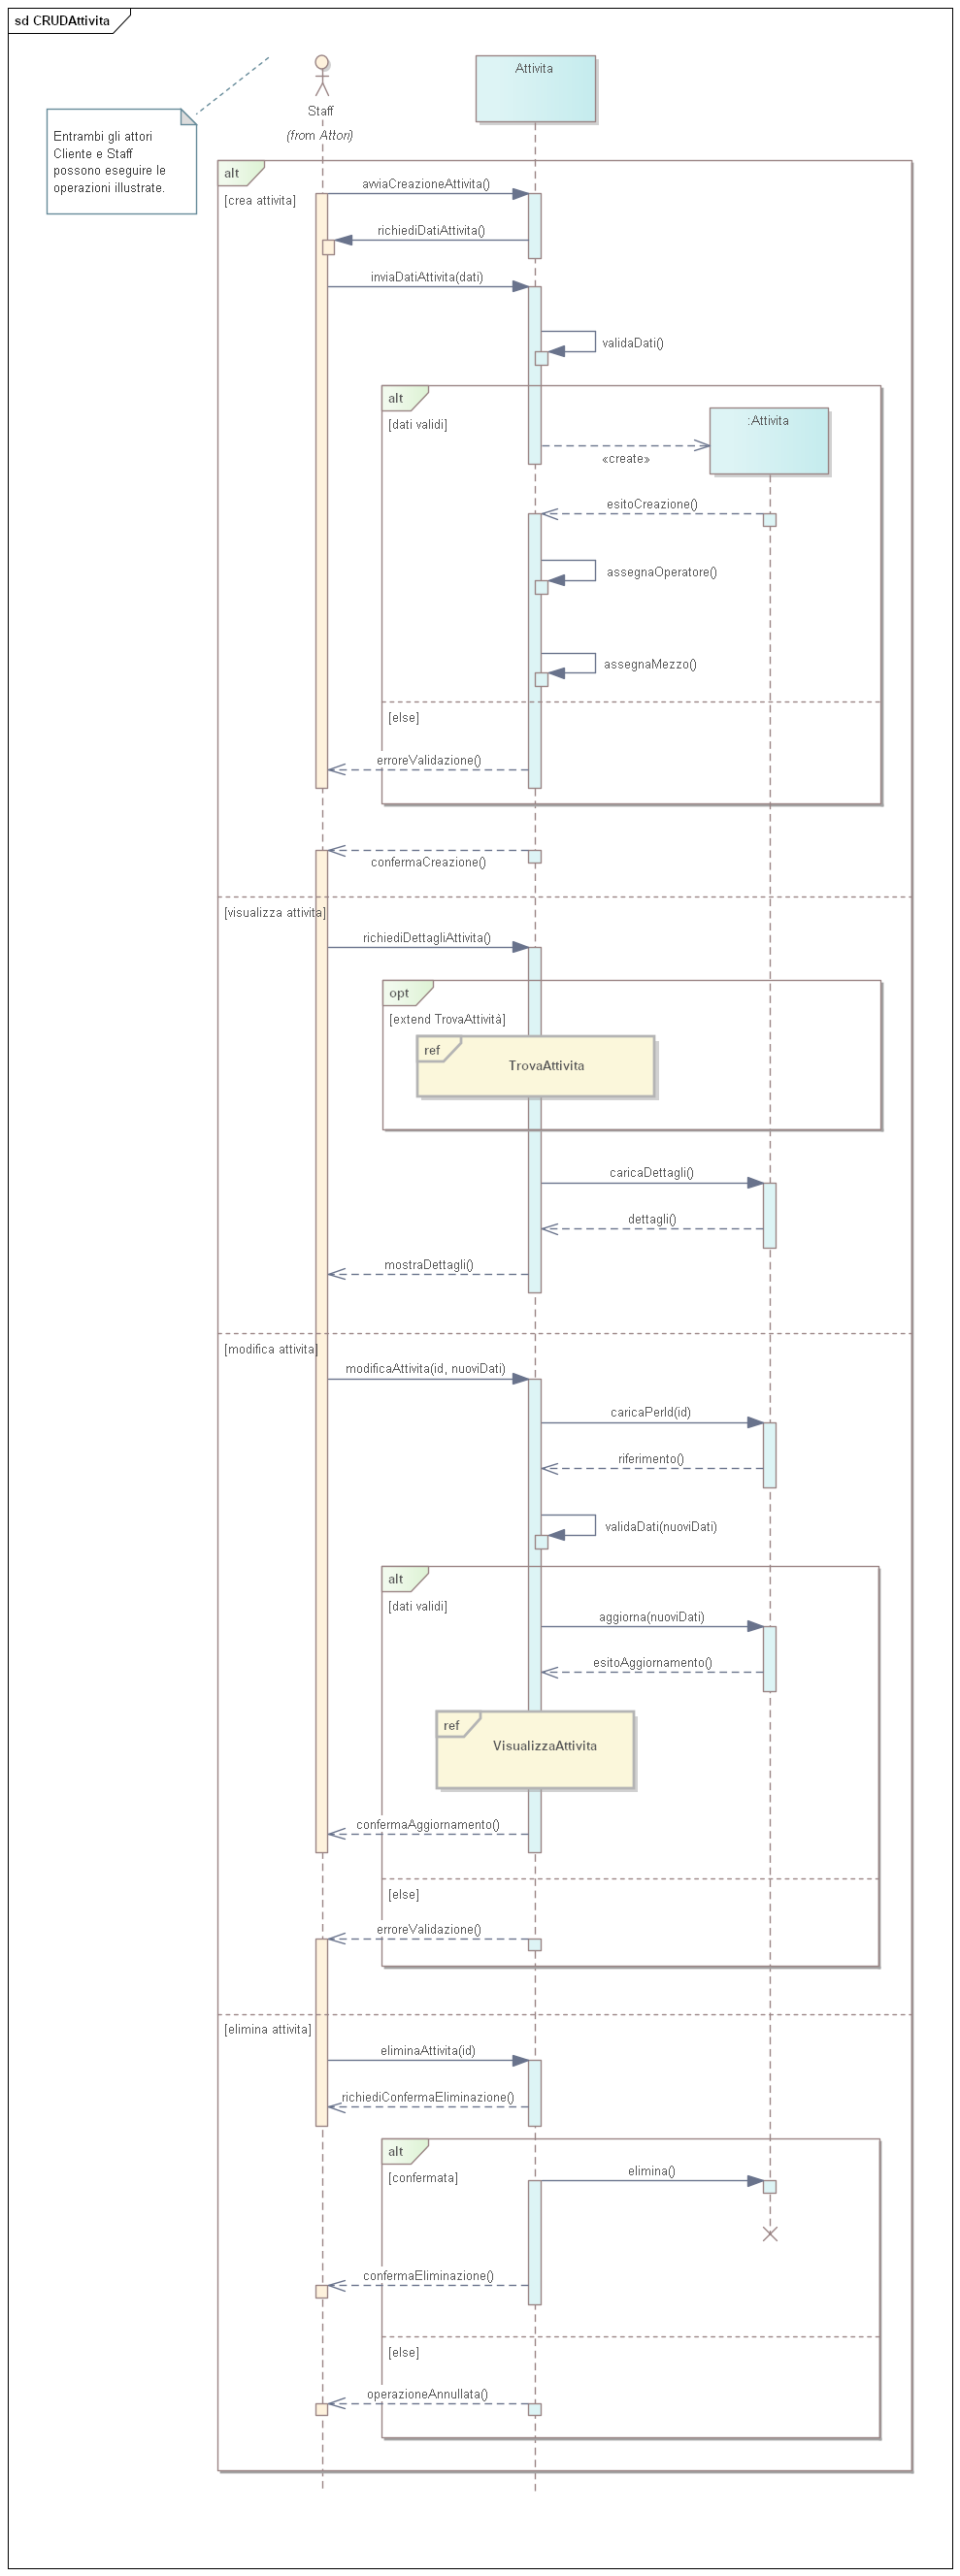
\includegraphics[width=\textwidth,trim=0 0 0 730pt,clip]{DiagrammaSequenzaCRUDAttivita}
\end{figure}

\clearpage
\newsubsection{Trova Documento}
\noindent
Il diagramma di sequenza illustra le interazioni tra l’operatore e il sistema per la ricerca di un documento tramite un criterio semplice. Viene evidenziata la validazione del criterio inserito e, se valido, la restituzione dei risultati corrispondenti. In alternativa, il sistema notifica l’assenza di documenti oppure segnala un errore se il criterio non è valido.

\begin{figure*}[!ht]
    \centering
    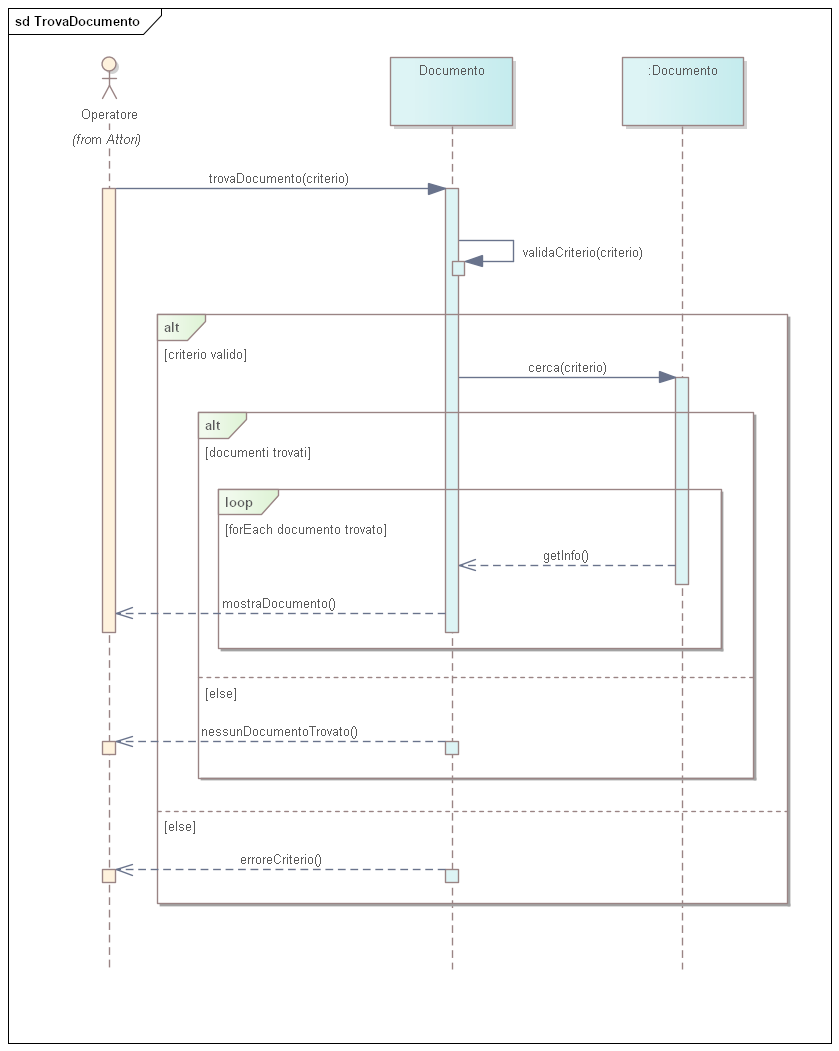
\includegraphics[width=1\textwidth]{DiagrammaSequenzaTrovaDocumento}
\end{figure*}

\clearpage
\newsubsection{Filtra Documento}
\noindent
Il diagramma di sequenza mostra il processo di filtraggio avanzato dei documenti, che estende il caso d’uso TrovaDocumento. Dopo la validazione dei criteri multipli, viene richiamata la logica di TrovaDocumento e successivamente applicati i filtri per restringere i risultati. L’operatore riceve così l’elenco dei documenti filtrati o, in alternativa, un messaggio di assenza di corrispondenze; in caso di criteri non validi, viene segnalato un errore.

\begin{figure*}[!ht]
    \centering
    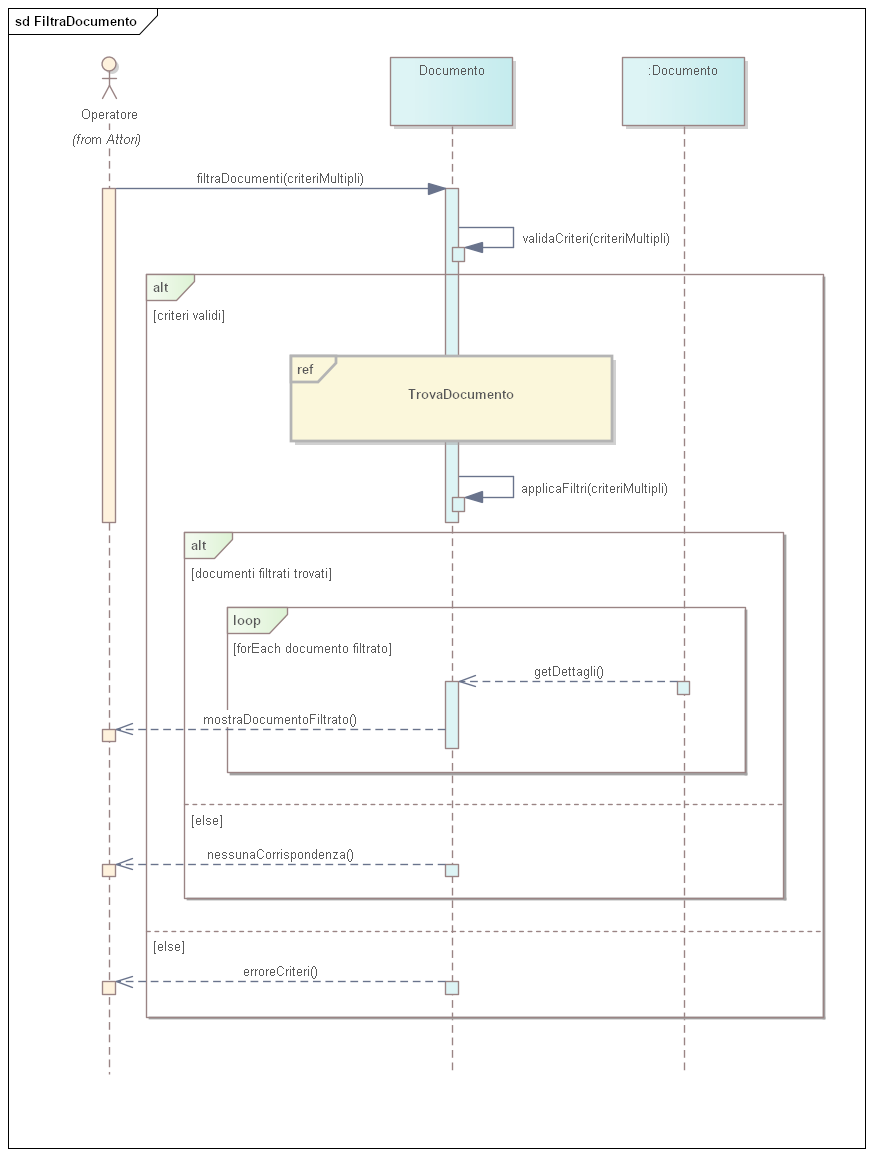
\includegraphics[width=1\textwidth]{DiagrammaSequenzaFiltraDocumento}
\end{figure*}

\clearpage
\newsection{Diagrammi di Attività}

\newsubsection{Login Utente}
Il diagramma rappresenta il processo di autenticazione di un utente. Dopo l’inserimento delle credenziali, il sistema le valida e consente l’accesso se corrette; altrimenti richiede un nuovo tentativo mostrando un messaggio di errore.

\begin{figure*}[!ht]
    \centering
    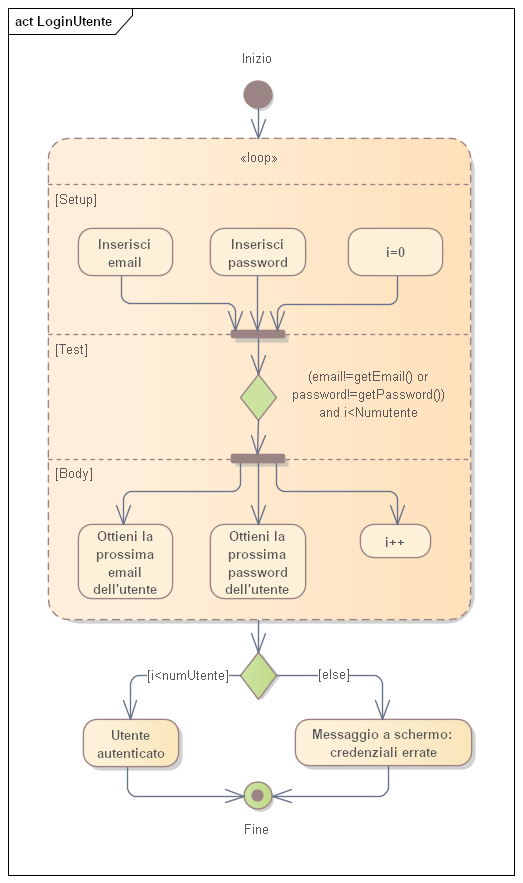
\includegraphics[width=0.78\textwidth]{DiagrammaAttivitaLoginUtente}
\end{figure*}

\clearpage
\newsubsection{Registrazione Utente}
Il diagramma mostra il processo di registrazione di un nuovo utente, sia da parte di un cliente sia da parte dello staff. Dopo l’inserimento dei dati, il sistema effettua la validazione e controlla l’unicità dell’email. In caso di errori o email già esistente, l’utente deve ripetere l’inserimento finché i dati non sono corretti. Solo dopo i controlli di validazione dell'email viene creato l’account con il ruolo appropriato e confermata l’avvenuta registrazione.

\begin{figure*}[!ht]
    \centering
    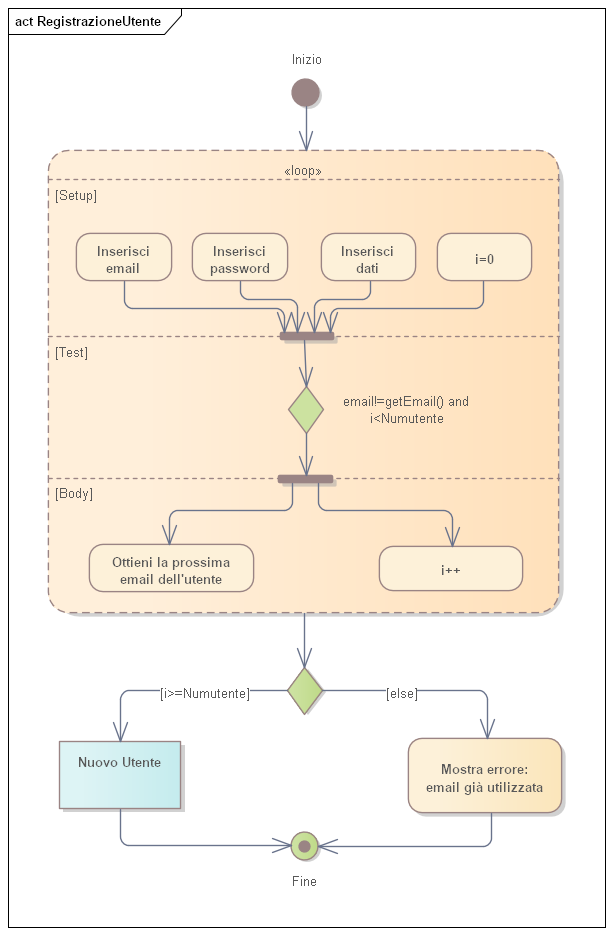
\includegraphics[width=0.78\textwidth]{DiagrammaAttivitaRegistrazioneUtente}
\end{figure*}

\clearpage
\newsubsection{CRUD Attività}
Il diagramma illustra la gestione completa delle attività attraverso operazioni di creazione, visualizzazione, modifica ed eliminazione. Le operazioni includono controlli di validazione e, se necessario, conferme da parte dell’utente. In fase di creazione sono previsti anche flussi quali l’assegnazione di un operatore e di un mezzo. Il diagramma evidenzia quindi le alternative e le condizioni che regolano il ciclo di vita di un’attività.

\begin{figure*}[!ht]
    \centering
    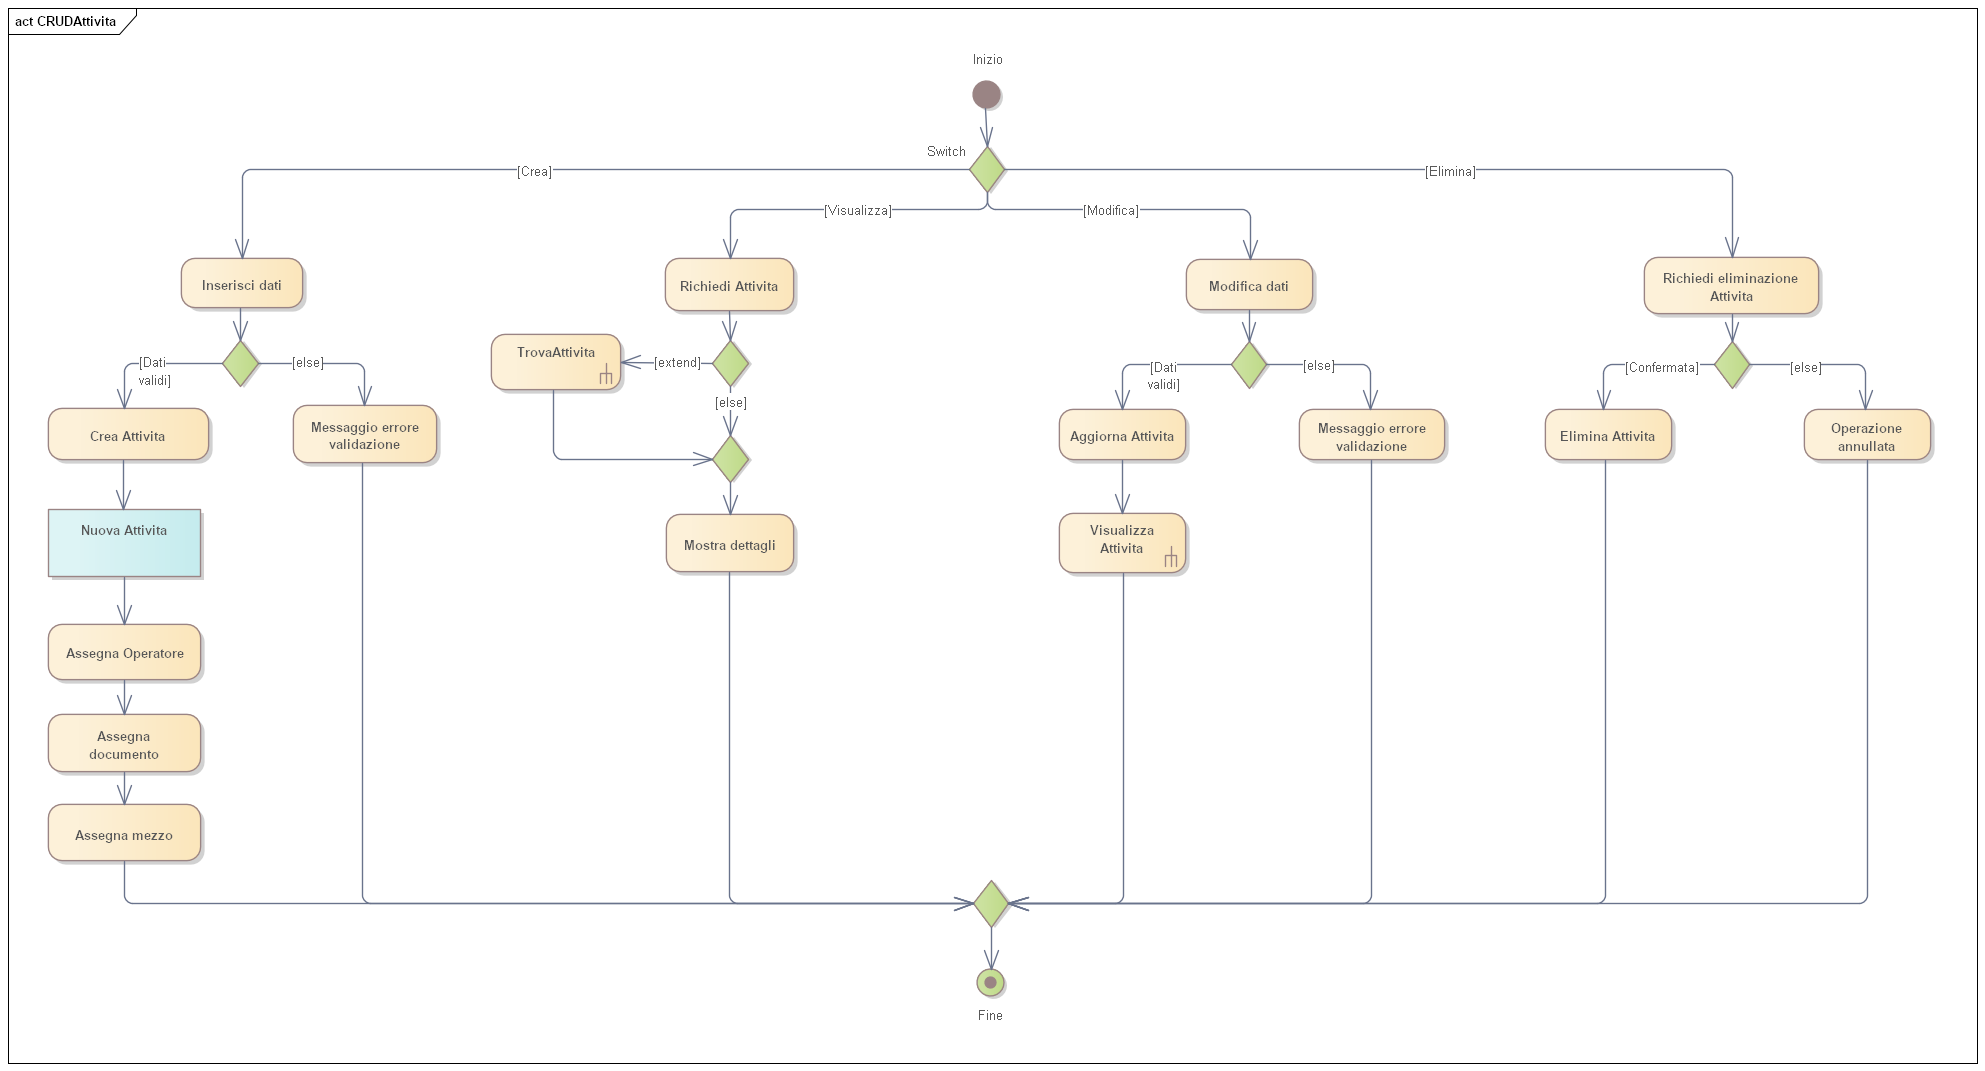
\includegraphics[width=1\textwidth]{DiagrammaAttivitaCRUDAttivita}
\end{figure*}

\clearpage
\newsubsection{Trova Documento}
Ricerca semplice basata su un singolo criterio: il sistema valida il criterio, restituisce l’elenco dei documenti trovati (iterando su ciascuno) o segnala l’assenza di risultati / l’errore di validazione.

\begin{figure*}[!ht]
    \centering
    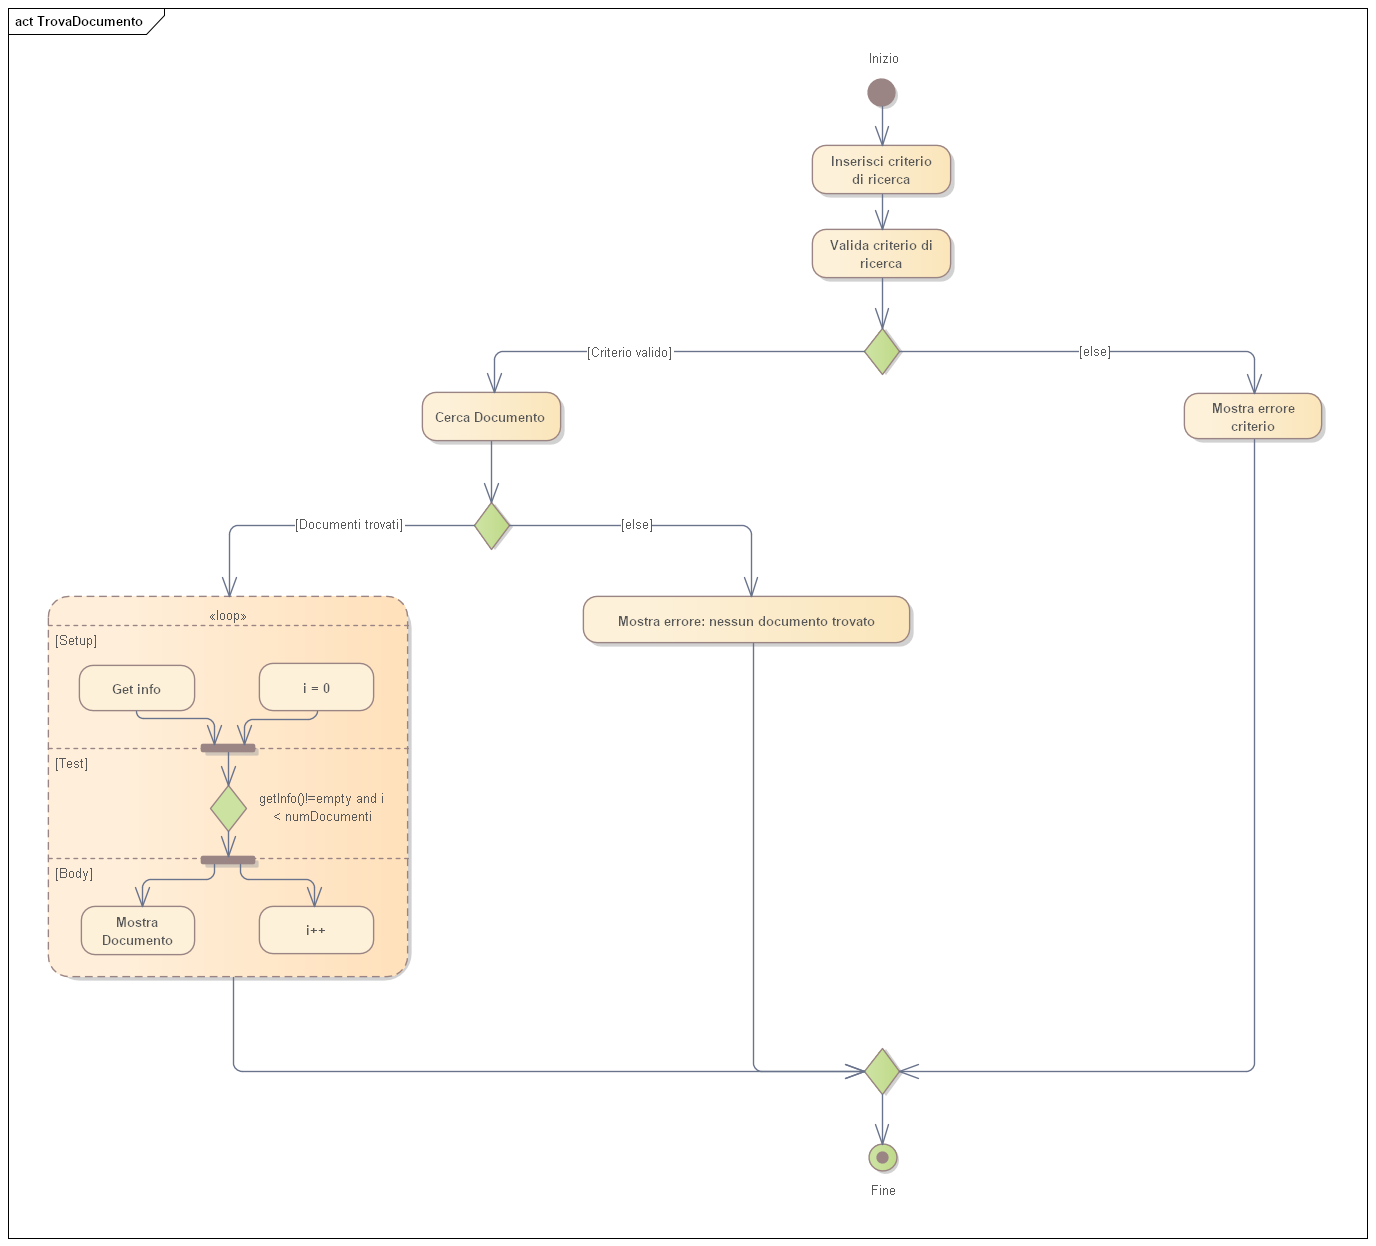
\includegraphics[width=1\textwidth]{DiagrammaAttivitaTrovaDocumento}
\end{figure*}

\clearpage
\newsubsection{Filtra Documento}
Filtraggio avanzato che estende la ricerca base: dopo la validazione dei criteri multipli viene eseguita la logica di TrovaDocumento e, se ci sono risultati base, si applicano i filtri avanzati per ottenere l’elenco finale o l’assenza di corrispondenze.

\begin{figure*}[!ht]
    \centering
    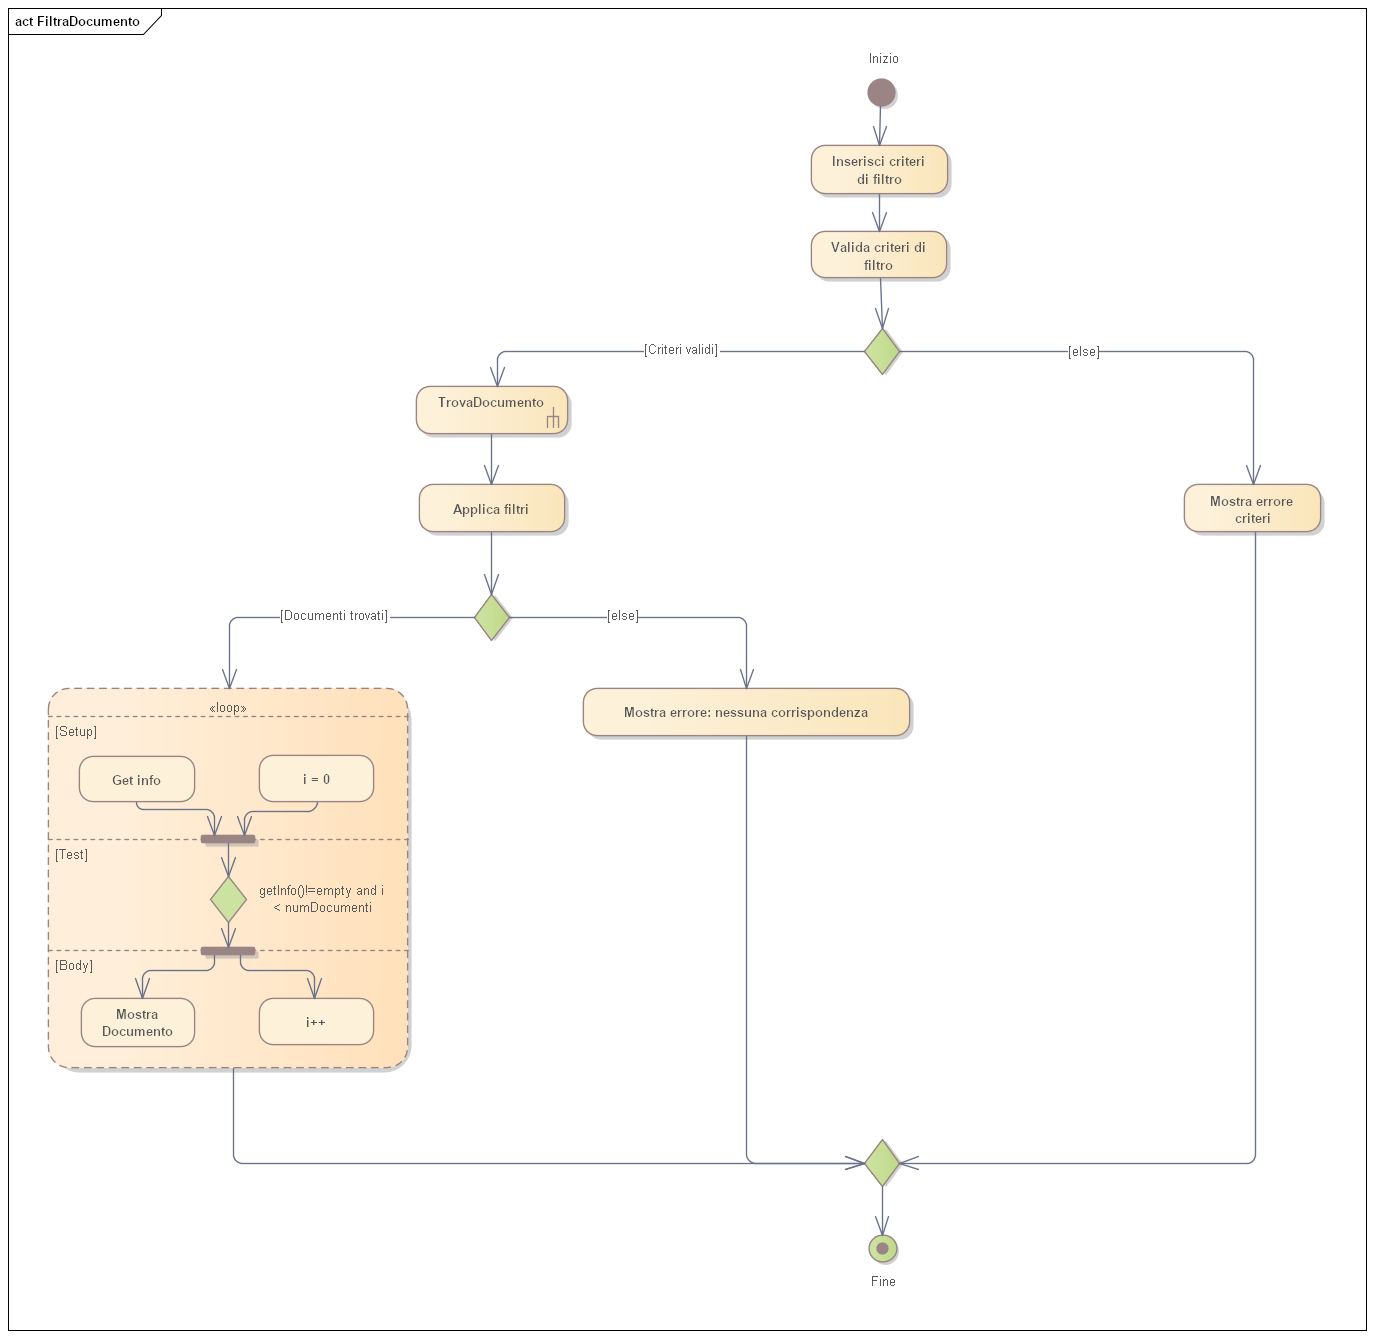
\includegraphics[width=1\textwidth]{DiagrammaAttivitaFiltraDocumento}
\end{figure*}

\newchapter{Progettazione}

\newsection{Diagrammi delle Classi di Progettazione}
\newsubsection{Package di Progettazione}
Il diagramma mostra la struttura dei package del sistema e le dipendenze tra i moduli principali, evidenziando come le classi siano organizzate per responsabilità.

\begin{figure*}[!ht]
    \centering
    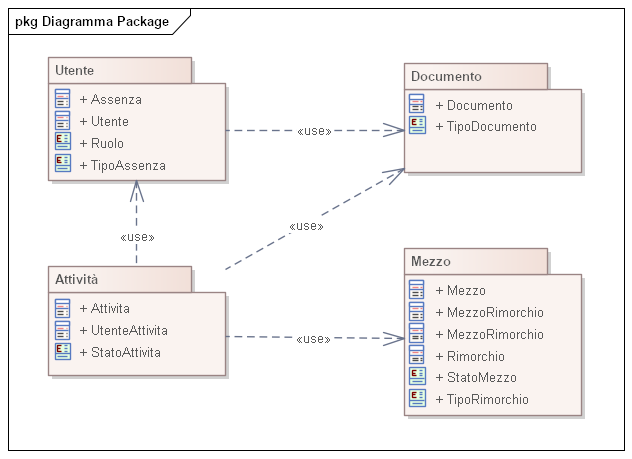
\includegraphics[width=1\textwidth]{DiagrammaPackageProgettazione}
\end{figure*}

\clearpage
\newsubsection{Classi di Progettazione: Utente}

Il diagramma delle classi di Utente e Assenza è una rappresentazione che riprende ed espande l'analisi iniziale. Le classi Utente e Assenza sono state arricchite con i dettagli di progettazione necessari per l'implementazione, inclusi attributi e metodi per la gestione e l'autenticazione.

\begin{figure*}[!ht]
    \centering
    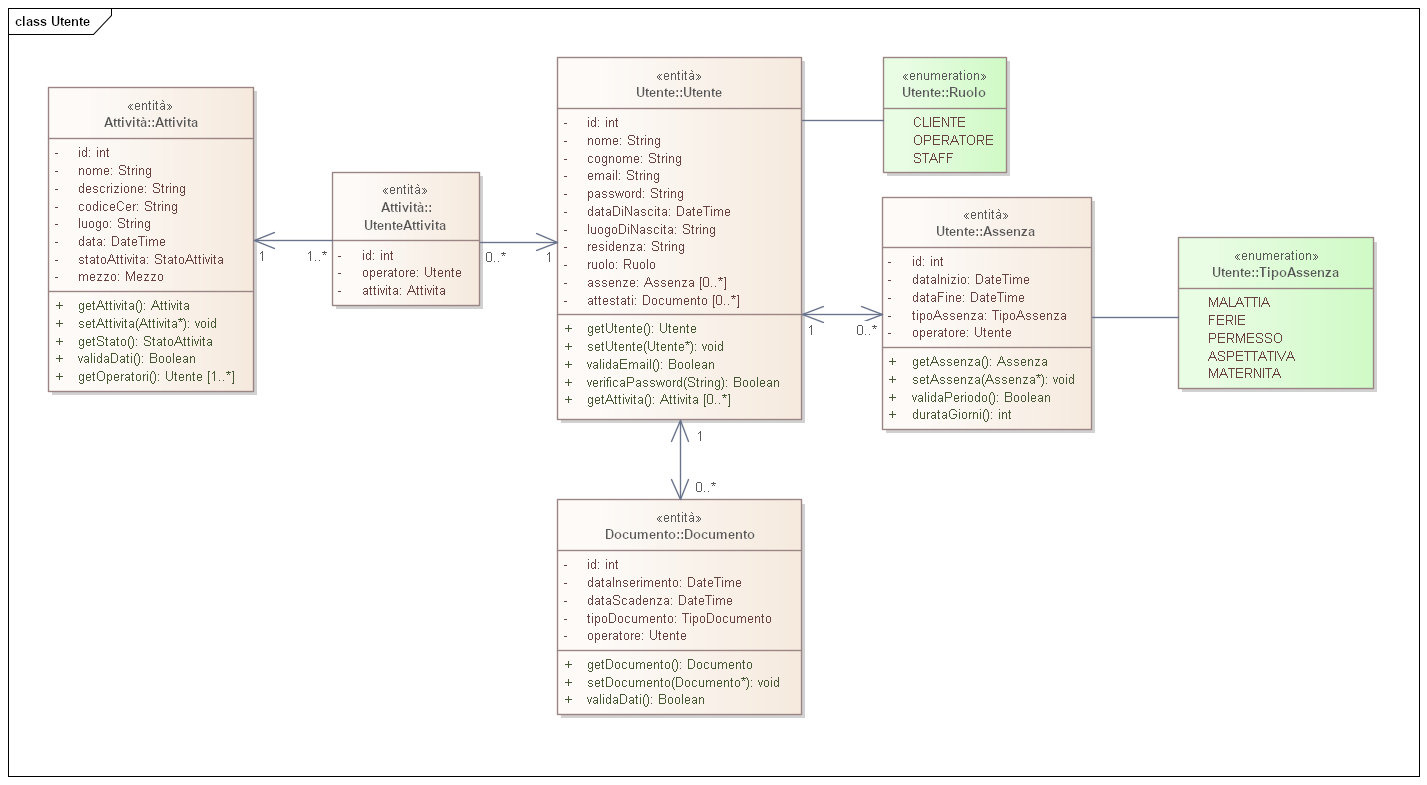
\includegraphics[width=1\textwidth]{DiagrammaClassiUtenteProgettazione}
\end{figure*}

\clearpage
\newsubsection{Classi di Progettazione: Mezzo}

Il diagramma delle classi di Mezzo riprende il modello di analisi e lo raffina per la fase di progettazione. Le classi Mezzo e la classe associata Rimorchio sono state arricchite con i dettagli necessari per l'implementazione, come gli attributi specifici e i metodi di gestione. Le associazioni con l'enumerazione per lo stato del veicolo rendono il modello una base solida per lo sviluppo.

\begin{figure*}[!ht]
    \centering
    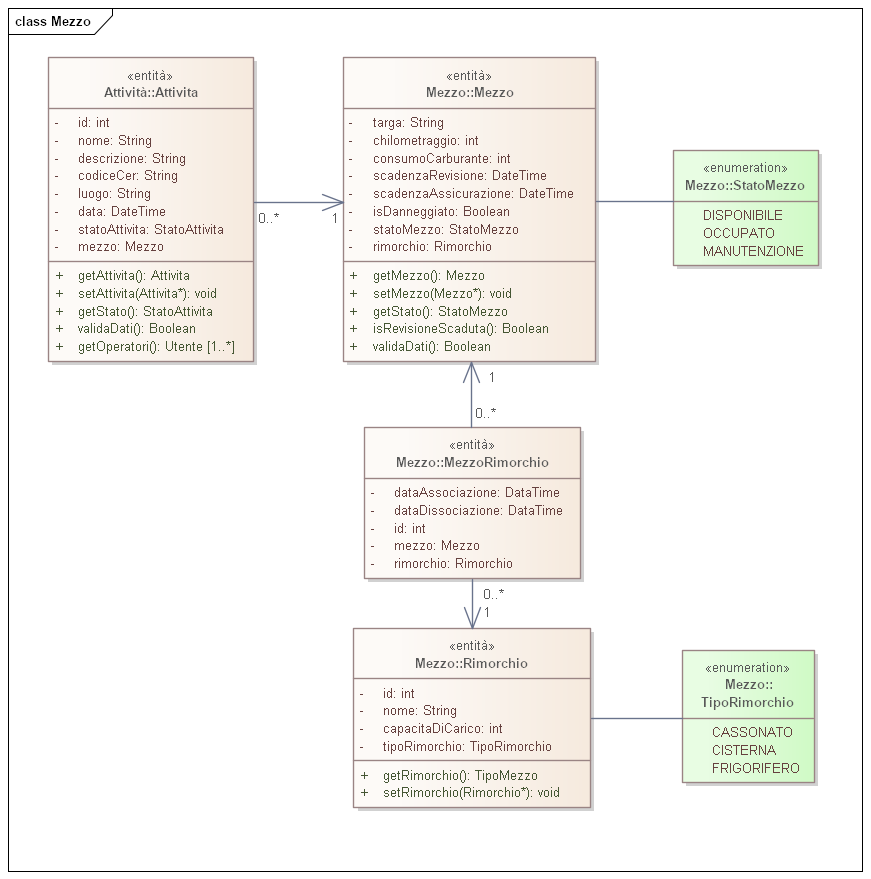
\includegraphics[width=1\textwidth]{DiagrammaClassiMezzoProgettazione}
\end{figure*}

\clearpage
\newsubsection{Classi di Progettazione: Attività}

Il diagramma delle classi di Attività è stato perfezionato per la progettazione. La classe Attività è stata arricchita con dettagli specifici e metodi di gestione. L'introduzione della classe intermedia UtenteAttivita risolve il legame molti a molti (many-to-many) tra Utente e Attività, rendendo il modello pronto per l'implementazione.

\begin{figure*}[!ht]
    \centering
    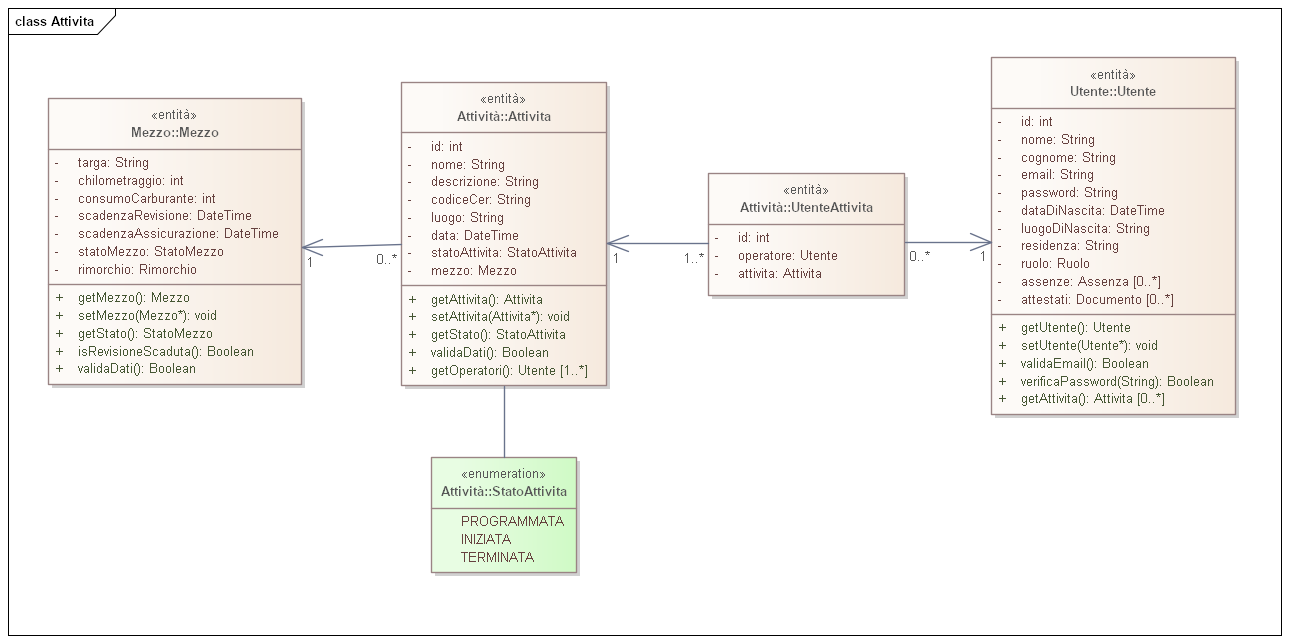
\includegraphics[width=1\textwidth]{DiagrammaClassiAttivitaProgettazione}
\end{figure*}

\clearpage
\newsubsection{Classi di Progettazione: Documento}
Il diagramma delle classi di Documento è un'evoluzione del modello di analisi. La classe Documento è stata arricchita con i dettagli di progettazione necessari, inclusi attributi e metodi per la gestione. Le associazioni con l'enumerazione per il tipo di documento rendono il modello una base solida per lo sviluppo.

\begin{figure*}[!ht]
    \centering
    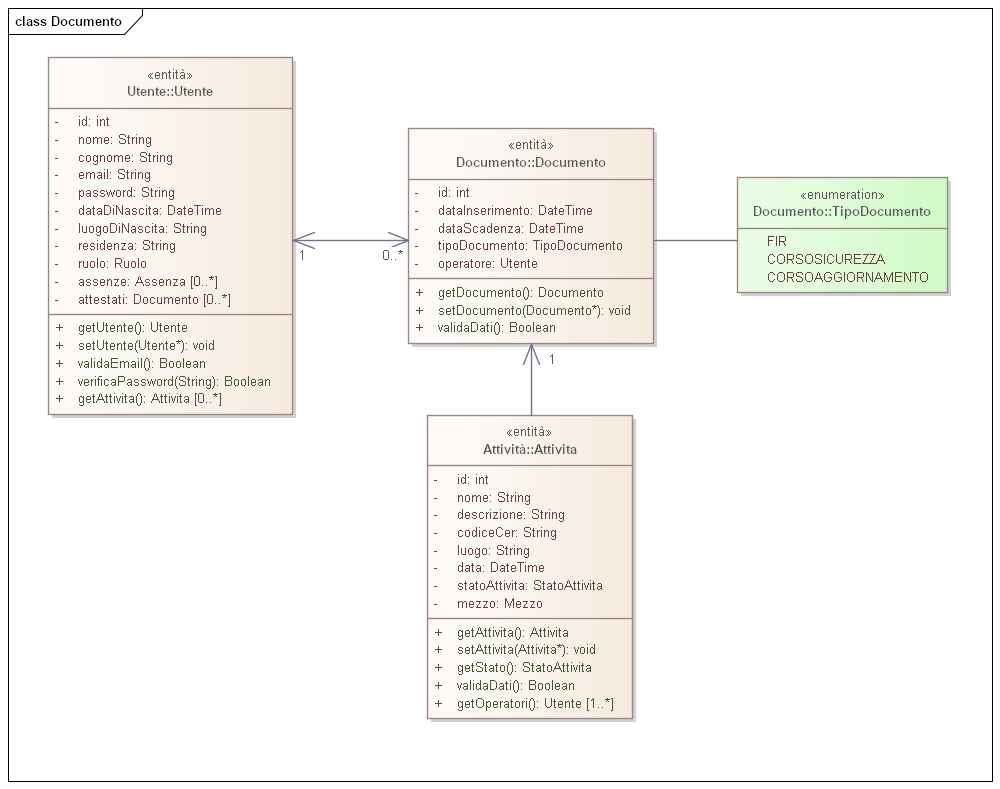
\includegraphics[width=1\textwidth]{DiagrammaClassiDocumentoProgettazione}
\end{figure*}

\clearpage
\newsubsection{Classi di Progettazione: Controllers}

Questo diagramma delle classi si discosta dagli altri, concentrandosi sull'architettura del software piuttosto che sul modello dati. Mostra i controller del sistema (es. UtenteController, MezzoController, ecc.), che fungono da intermediari tra l'interfaccia utente e le entità. Le relazioni tra i controller e le rispettive entità (es. Utente, Mezzo, ecc.) sono indicate con una dipendenza (<use>), evidenziando che i controller utilizzano le entità per svolgere le loro funzioni. Questo modello illustra la separazione dei compiti a un livello più alto, cruciale per l'organizzazione del codice e la manutenzione.

\begin{figure*}[!ht]
    \centering
    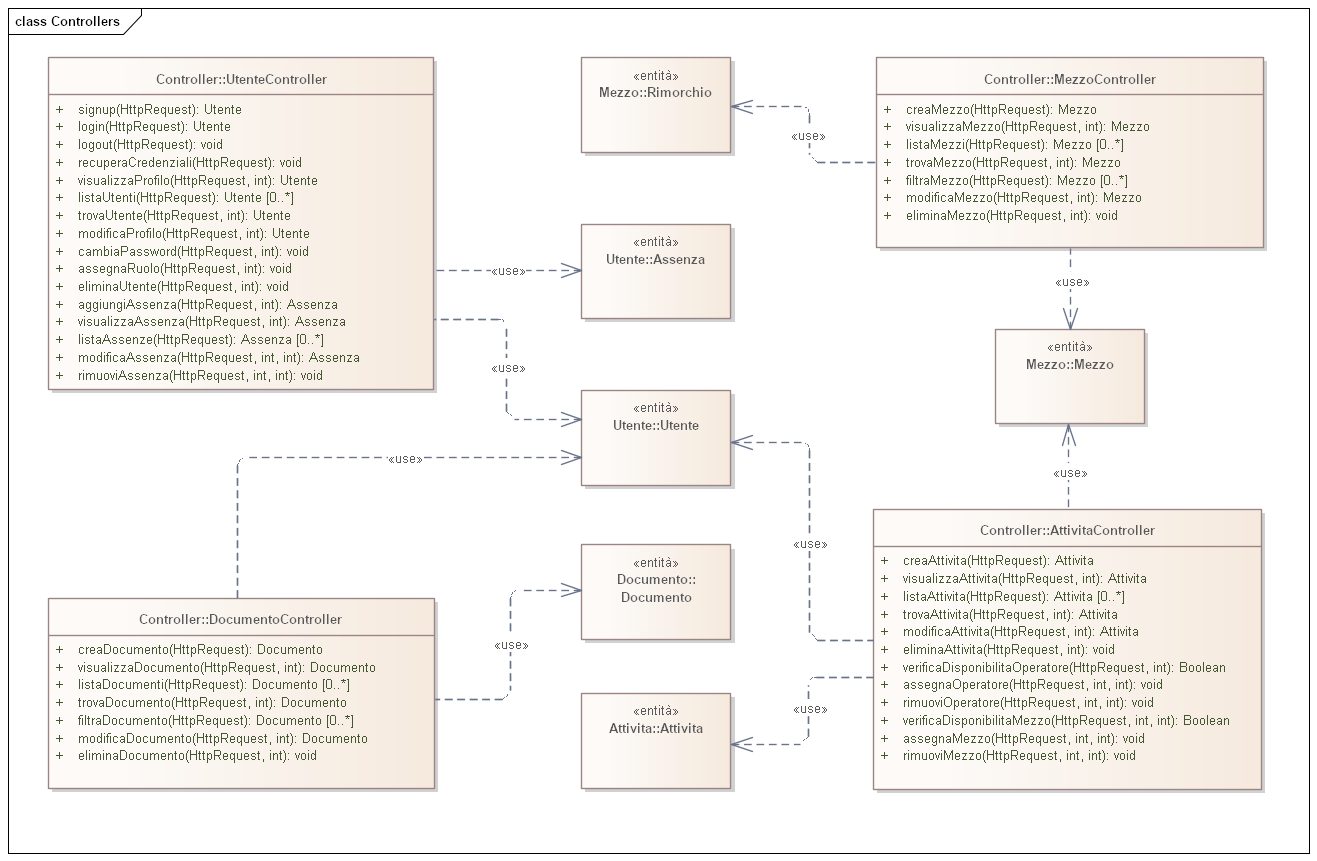
\includegraphics[width=1\textwidth]{DiagrammaClassiControllersProgettazione}
\end{figure*}

\clearpage
\newsection{Diagramma dei Componenti}
Questo diagramma illustra l'architettura di alto livello del sistema, focalizzandosi sulle dipendenze tra i suoi componenti. Si evidenzia che le entità di dominio, come Utente, Attività, Mezzo e Documento, non interagiscono direttamente tra loro, ma delegano la loro logica a un insieme di Controller. I controller (UtenteController, AttivitaController, MezzoController, DocumentoController) espongono delle interfacce che sono utilizzate per separare la logica applicativa dalla gestione dei dati. 

\begin{figure*}[!ht]
    \centering
    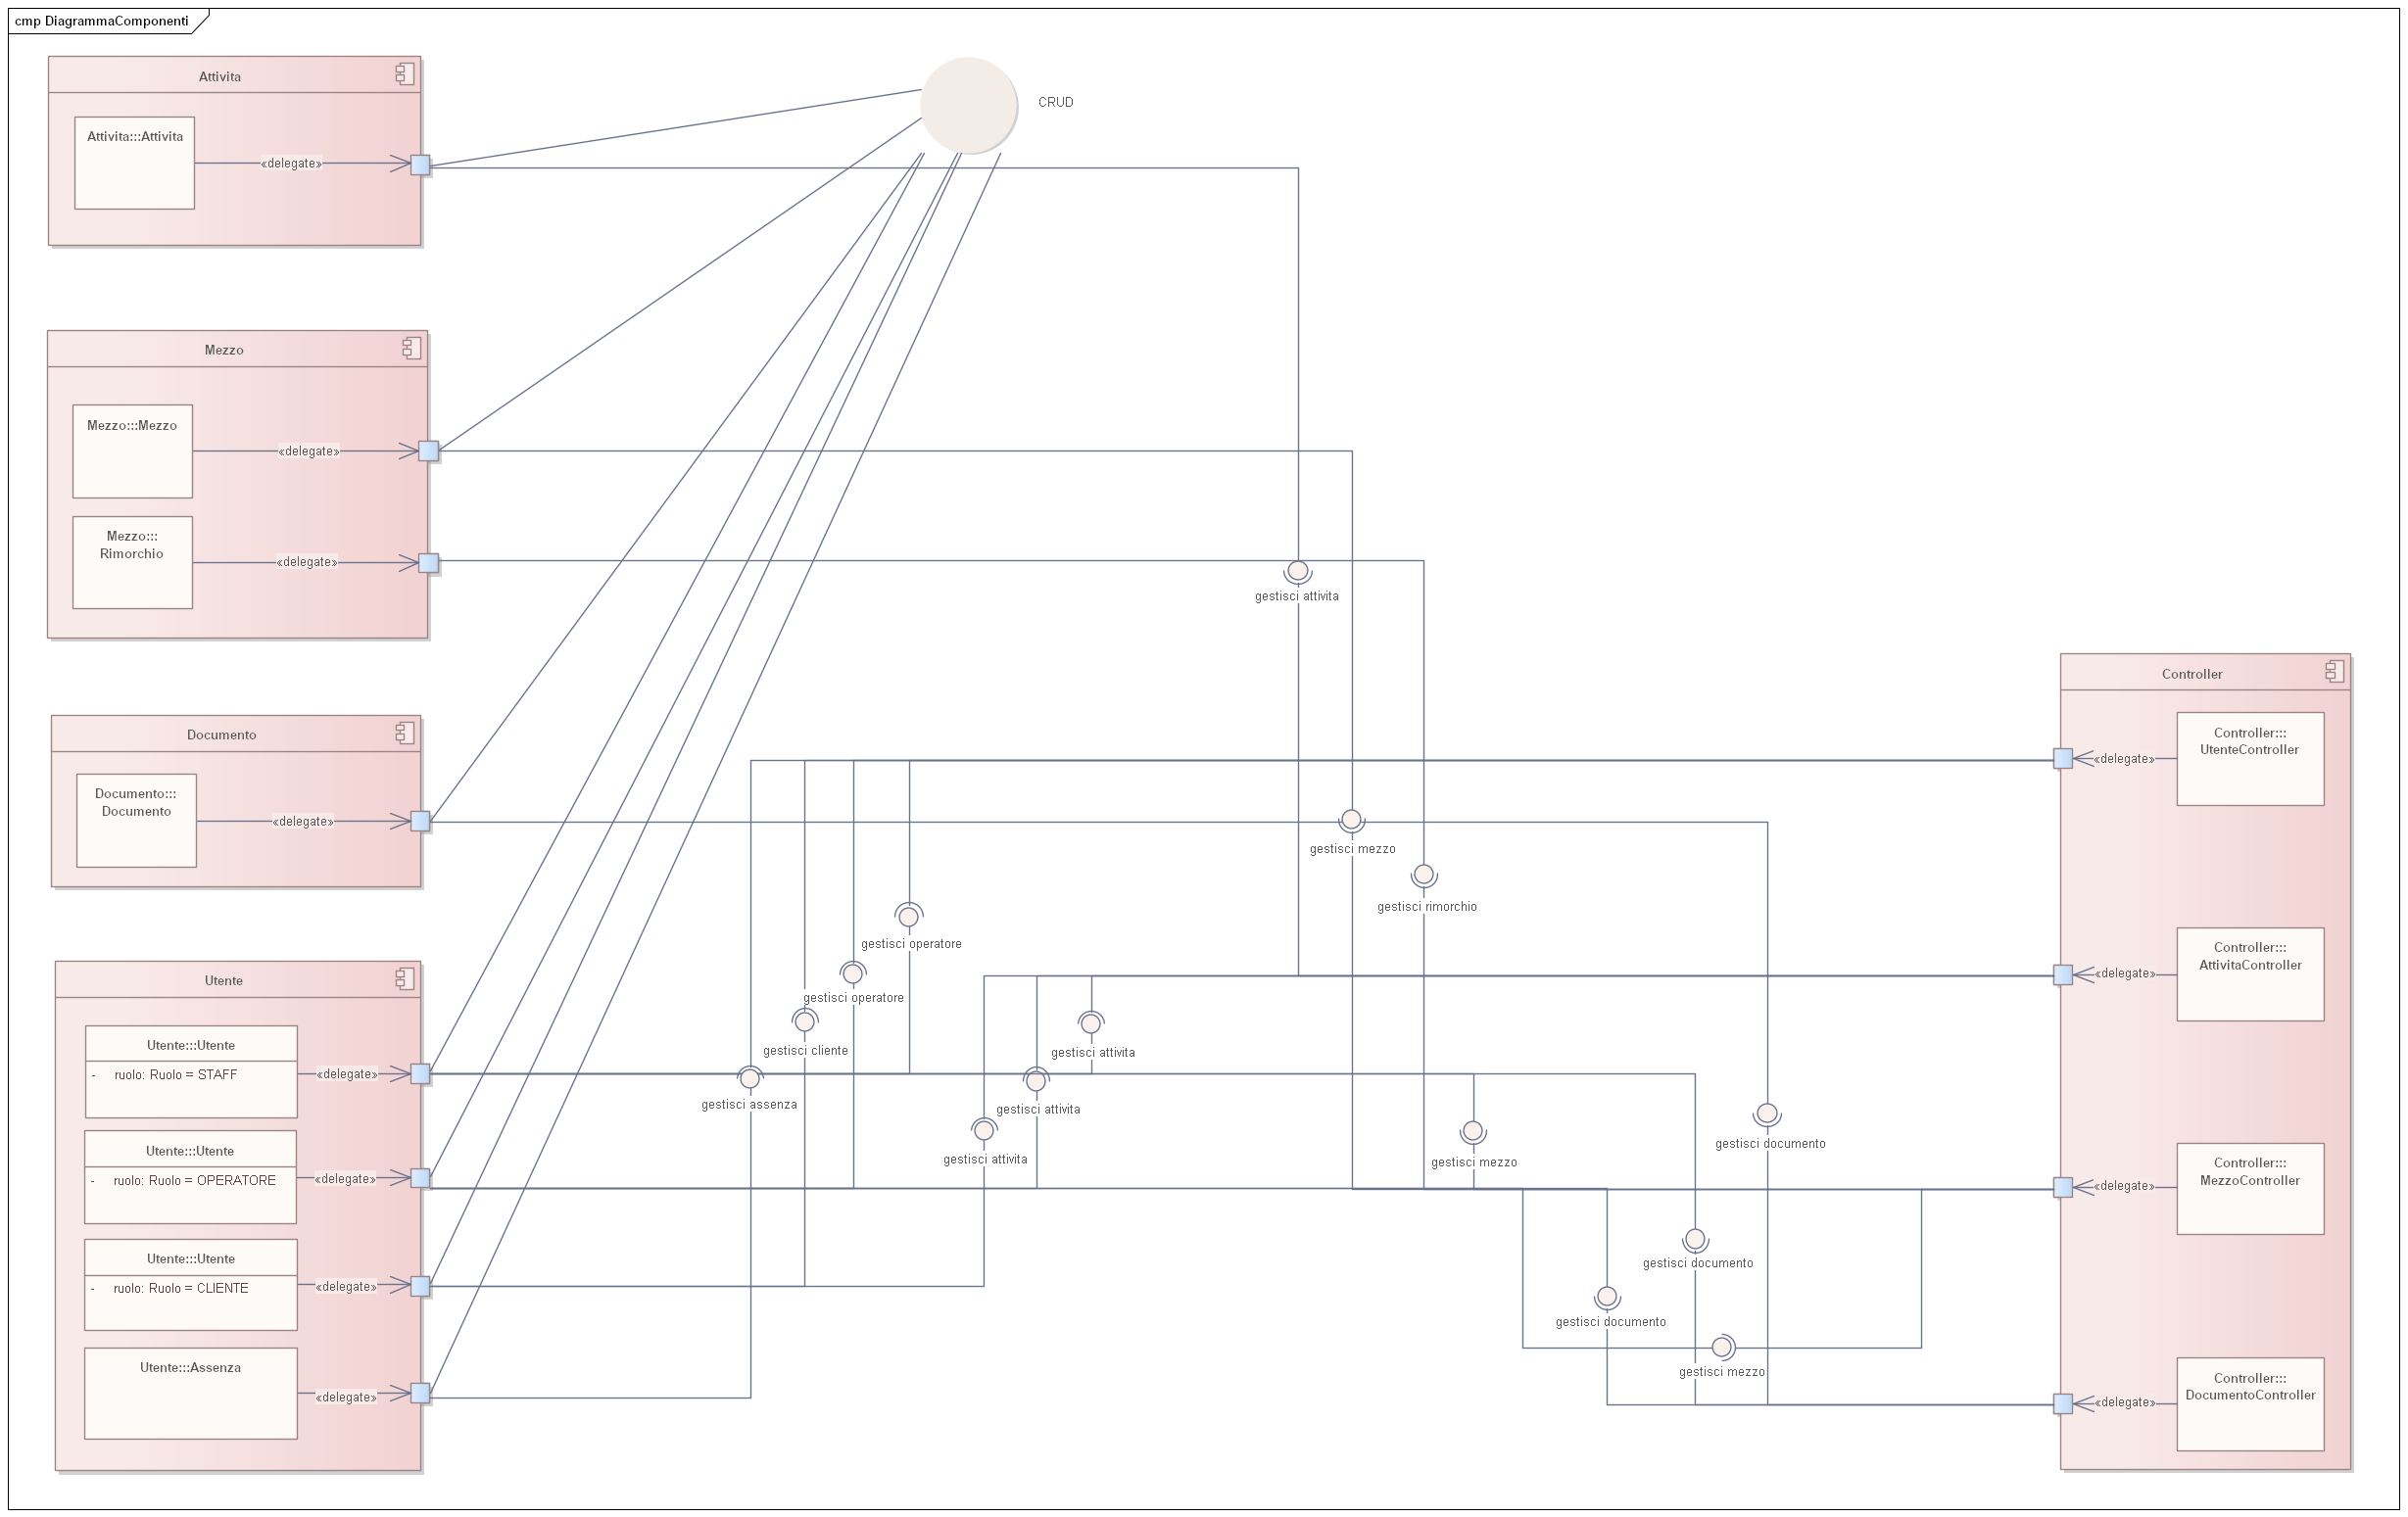
\includegraphics[width=1\textwidth]{DiagrammaComponenti}
\end{figure*}

\clearpage
\newsection{Diagrammi delle Macchine a Stati}

\newsubsection{Macchine a Stati: Attività}
Questo diagramma di stato modella il ciclo di vita di un'attività. L'attività inizia nello stato Programmata e passa allo stato Iniziata solo quando la sua data coincide con quella odierna. L'attività si sposta quindi nello stato Terminata solo dopo che il documento "FIR" (Foglio di Itinerario e Registro) corrispondente è stato caricato. Il diagramma mostra un flusso sequenziale ma, come in tutti i diagrammi di stato, un'uscita dal sistema può verificarsi in qualsiasi momento. Se un'attività viene eliminata, il suo stato si conclude, rappresentato nel diagramma dal simbolo Exit, che indica la terminazione del ciclo di vita dell'oggetto.

\begin{figure*}[!ht]
    \centering
    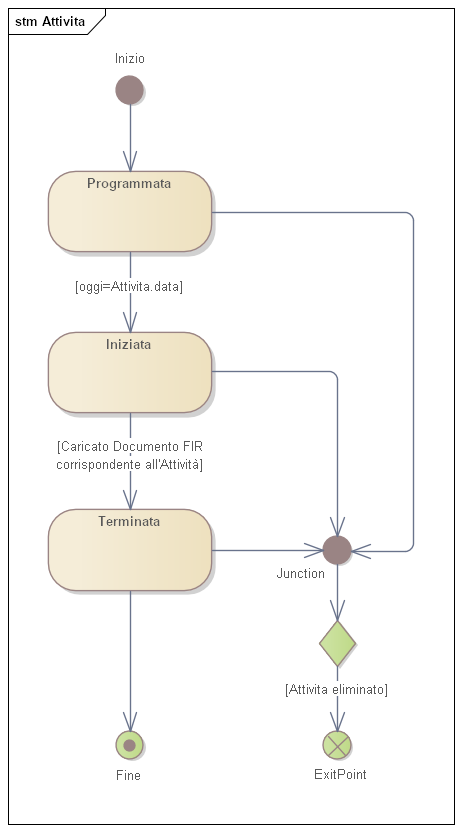
\includegraphics[width=0.67\textwidth]{DiagrammaMacchineStatiAttivita}
\end{figure*}

\clearpage
\newsubsection{Macchine a Stati: Mezzo}
Questo diagramma di stato modella il ciclo di vita completo di un mezzo. Il mezzo inizia nello stato Disponibile e passa allo stato Occupato quando viene assegnato a un'attività. Al termine dell'attività, il mezzo ritorna allo stato Disponibile, pronto per una nuova assegnazione. Se il mezzo si danneggia o la condizione scadenzaRevisione < oggi viene verificata come vera, il mezzo entra nello stato di Manutenzione, per poi tornare nuovamente Disponibile una volta che i lavori sono stati completati. In ogni momento, se il mezzo viene eliminato dal sistema, il suo stato si conclude, come rappresentato dal simbolo ExitPoint nel diagramma UML, che indica la terminazione del ciclo di vita dell'oggetto.

\begin{figure*}[!ht]
    \centering
    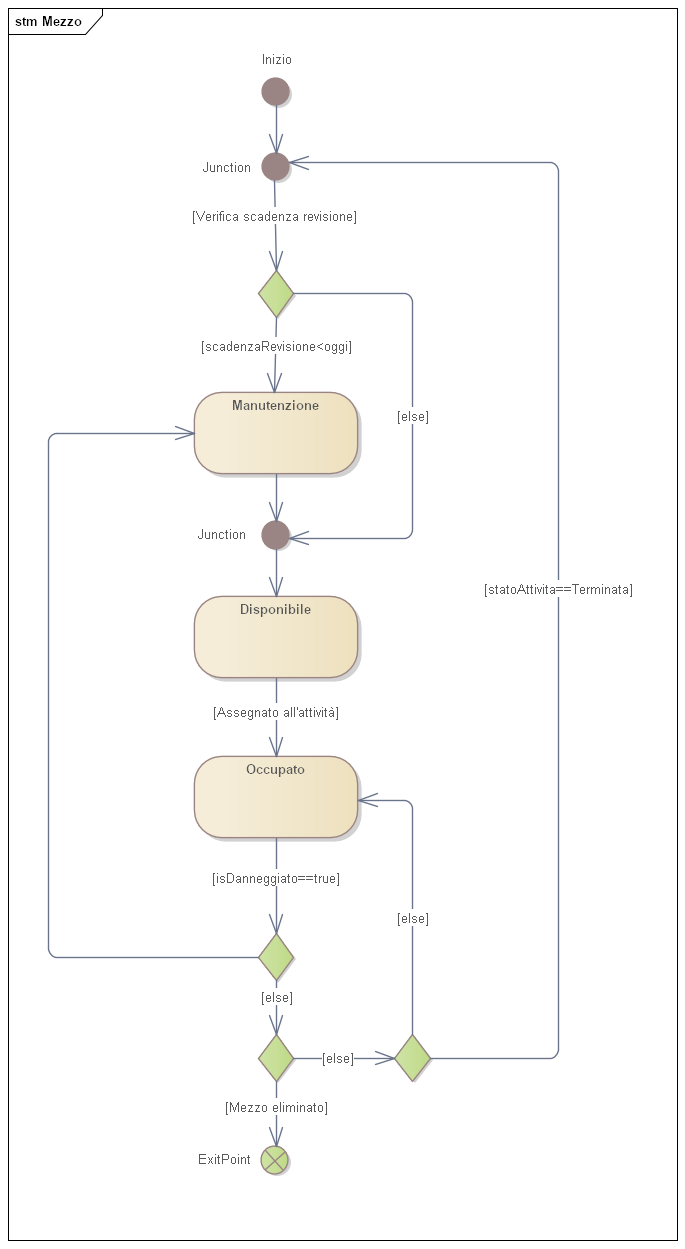
\includegraphics[width=0.66\textwidth]{DiagrammaMacchineStatiMezzo}
\end{figure*}

\end{document}
